% !TeX root = main.tex
\documentclass[12pt, a4paper, twoside]{report}   % Tamaño de papel, de fuente y márgenes

\usepackage{shellesc}
 
\usepackage[spanish,es-ucroman]{babel}  % Idioma y codificación, para poder usar
\usepackage[T1]{fontenc}
% \usepackage[utf8x]{inputenc} % tildes, eñes, etc., sin problemas\usepackage{newunicodechar}
\usepackage{array}

% Para tablas dinámicas
\usepackage{tabularx}
\usepackage{longtable}

% Para fijar el interlineado
\usepackage{setspace} 

% Para los encabezados y pies
\usepackage{fancyhdr}

% Para generar texto como contenido de prueba, se puede eliminar en la memoria final
\usepackage{lipsum}
\usepackage{blindtext}

% Para fuentes (Using common PostScript fonts with LaTeX)
\usepackage{helvet}
\usepackage{wallpaper}                  % Para introducir el PDF con la portada EPSJ
\usepackage[absolute,overlay]{textpos}  % 
\usepackage{etoolbox}                   % Herramientas de logica, variables y condicionales y bibliografía
\usepackage[numbers]{natbib}            % Para gestionar la bibliografia
\usepackage{csquotes}                   % 
\usepackage{hyperref}                   % Para URL como enlaces
\usepackage{booktabs}                   % Para tablas con mejor apariencia
\usepackage{listings}                   % Para incluir listados de código

% Para los emojis, debes compilar el paquete
\usepackage{twemojis}

% El paquete parte de las facilidades básicas del paquete de color 
\usepackage{xcolor}     
% \usepackage{algorithm}
% \usepackage{algpseudocode}                
\usepackage[linesnumbered, ruled,vlined]{algorithm2e}  % https://ctan.javinator9889.com/macros/latex/contrib/algorithm2e/doc/algorithm2e.pdf
\usepackage[acronym]{glossaries}        %
\usepackage{pdflscape}                  %
\usepackage{rotating}
\usepackage[paper=portrait,pagesize]{typearea}

% Bug Underfull \hbox (badness 10000)LaTeX
% \usepackage{parskip}
% Controlar la enumeración de los titulos
\usepackage{titlesec}
\usepackage{etoc}       
\setcounter{tocdepth}{4}
\setcounter{secnumdepth}{4}

\titleformat{\paragraph}{\normalfont\normalsize\bfseries}{\theparagraph}{1em}{}\titlespacing*{\paragraph}{0pt}{3.25ex plus 1ex minus .2ex}{1.5ex plus .2ex}

% 
\usepackage{ifluatex}
\ifluatex
  \usepackage{pdftexcmds}
  \makeatletter
  \let\pdfstrcmp\pdf@strcmp
  \let\pdffilemoddate\pdf@filemoddate
  \makeatother
\fi

% Para las imágenes
\usepackage{svg}                  % Enable --shell-escape for external commands
% \setsvg{inkscapeexe=inkscape, inkscapeopt=-z -D}     
\usepackage{wrapfig}                   
\usepackage{float}                     
\raggedbottom 

  
% Gestion de los tamaños de las páginas
\usepackage{geometry}                   % https://www.ctan.org/pkg/geometry
\usepackage{fancyhdr}                   % https://www.ctan.org/pkg/fancyhdr

\usepackage{setspace}                   %for doublespacing
\doublespacing %double spacing
\geometry{
  a4paper,
  left=1.5in,
  right=1.5in,
  top=1in,
  bottom=1in,
  margin=2.5cm,
  heightrounded,
}
 
% \usepackage[acronym,nomain,toc,automake]{glossaries-extra}
% \usepackage[acronym,toc=true,nomain,xindy]{glossaries-extra}
% \setabbreviationstyle[acronym]{long-short} 

\usepackage{csvsimple}                  % https://www.ctan.org/pkg/csvsimple
\usepackage{amsmath}                    % https://www.ctan.org/pkg/amsmath
\usepackage{actuarialangle}
\usepackage{amssymb}
\usepackage{mathtools}
\usepackage{bm}

\usepackage{commath}
\usepackage{bookmark} 
% Para figuras y espacios centrados con tamaño de linea pequeño y alineada las lineas
\usepackage[justification=centering,font=footnotesize]{caption}
\usepackage{subcaption}
\usepackage{varwidth}
\DeclareCaptionFormat{varwidth}{%
  \begin{varwidth}{\linewidth}#1#2#3\end{varwidth}%
}
\captionsetup{format=varwidth}

% VTimeline
\usepackage{charter} 
\usepackage{environ}
\usepackage{tikz}
\usetikzlibrary{calc,matrix}
\usepackage{pgfplots}
\pgfplotsset{compat=every axis/.append style={tick label style={/pgf/number format/fixed},font=\scriptsize,ylabel near ticks,xlabel near ticks,grid=major}}

\usepackage{amsthm}
\newtheorem{theorem}{Teoremas}[section]
\newtheorem{lemma}[theorem]{Lemma}

\usepackage{enumitem}
\setlist{nolistsep}

\usepackage{tikz} 
\usetikzlibrary{calc}

\newcommand{\addterm}[7][]{%
  \newglossaryentry{#2}{name={\textit{#3} (angl.\ \textit{#5})},
     first={\textit{#3} (angl.\ \textit{#5})},
     firstplural={\textit{#4} (angl.\ \textit{#6})},
     text={#3},
     plural={#4},
     sort={#3},
     description={#7},#1}%
}


% ==== Introducir aquí el nombre del estudiante
\def\Estudiante{Antonio Mudarra Machuca}

% ==== Introducir aquí el nombre de los tutores. Si solo hay uno dejar las llaves de \TutorB vacías
\def\TutorA{Antonio Jesús Rivera Rivas}
\def\TutorB{María José del Jesus Díaz}
\def\Departamento{Departamento de informática}

% ==== Introducir aquí el título de completo y abreviado (para las cabeceras) del TFG
\def\TituloTFG{Redes neuronales adversarias en seguridad informática}
\def\TituloAbreviado{RNASI}

% ==== Introducir aquí el mes y año de presentación del TFG
\def\Fecha{septiembre de 2023}
\def\FechaPortada{septiembre, 2023}

% Configuración idioma
\renewcommand{\spanishtablename}{Tabla.}  % Título para las tablas
\renewcommand{\spanishcontentsname}{Tabla de contenidos}  % y los índices
\renewcommand{\spanishlistfigurename}{Lista de figuras}
\renewcommand{\spanishlisttablename}{Lista de tablas}

\renewcommand{\algorithmcfname}{Algoritmo}
\renewcommand{\listalgorithmcfname}{Lista de algoritmos}
\renewcommand{\lstlistingname}{Listado}
\renewcommand{\lstlistlistingname}{Lista de listados de código}

% Hoy en día la Inteligencia Artificial y sus aplicaciones están cada vez más implantadas en diferentes sistemas de nuestra sociedad. Dentro de esta disciplina el destacan el campo del Machine Learning (Aprendizaje Automático), donde como resultado de aplicar algoritmos de aprendizaje a datos se obtienen modelos que destacan por los resultados que obtienen. Gracias a su precisión estos modelos se encuentran desplegados en sistemas informáticos de gran importancia y que contralan procesos en diversos ámbitos de nuestra vida.

% Evidentemente estos sistemas pueden son vulnerables ataques de seguridad siendo los denominados modelos adversarios (basados normalmente en redes neuronales) los que suelen estar implicados tanto en estos ataques como en el posible robustecimiento de los sistemas atacados y por tanto de los modelos de aprendizaje automático en los que se basan. El objetivo de este trabajo es hacer un estudio bibliográfico del campo de los modelos adversarios aplicados a la seguridad informática. Posteriormente se elegirá un área aplicación, con sus respectivos conjuntos de datos y modelos representativos. Se realizarán experimentaciones en este área y se analizarán los resultados.

% Configuración tabularX
\newcolumntype{Y}{>{\centering\arraybackslash}X}



\hypersetup{
    colorlinks=true,
    linkcolor=blue,
    filecolor=magenta,
    urlcolor=cyan,
    pdftitle={\TituloTFG},
    pdfauthor={\Estudiante}
    bookmarks=true,
    bookmarksopen=true,
    pdfpagemode=FullScreen,
    breaklinks=true,
    citecolor=cyan,
}


\lstset{ %
    %language=delphi,                % the language of the code
    basicstyle=\linespread{0.7}\small\ttfamily,       % the size of the fonts that are used for the code
    numbers=left,                   % where to put the line-numbers
    numberstyle=\footnotesize\color{gray},  % the style that is used for the line-numbers
    stepnumber=1,                   % the step between two line-numbers. If it's 1, each line will be numbered
    numbersep=7pt,                  % how far the line-numbers are from the code
    backgroundcolor=\color{gray!5},  % choose the background color. You must add \usepackage{color}
    showspaces=false,               % show spaces adding particular underscores
    showstringspaces=true,         % underline spaces within strings
    showtabs=true,                 % show tabs within strings adding particular underscores
    frameround=fttt,
    frame=rtBL,                   % adds a frame around the code
    rulecolor=\color{black},        % if not set, the frame-color may be changed on line-breaks within not-black text (e.g. commens (green here))
    tabsize=4,                      % sets default tabsize to 2 spaces
    aboveskip=1em,
    captionpos=b,                   % sets the caption-position to bottom
    breaklines=true,                % sets automatic line breaking
    breakatwhitespace=false,        % sets if automatic breaks should only happen at whitespace
    title=\lstname,                 % show the filename of files included with \lstinputlisting;  also try caption instead of title
    keywordstyle=\bf\ttfamily,          % keyword style
    commentstyle=\color{black!60}\ttfamily,       % comment style
    stringstyle=\color{blue}\ttfamily,         % string literal style
    escapeinside={\%*}{*)}            % if you want to add a comment within your code
}

\lstset
{
    language=[LaTeX]TeX,
    breaklines=true,
    basicstyle=\tt\scriptsize,
    keywordstyle=\color{blue},
    identifierstyle=\color{gray},
    texcl=true
}
\lstset{
language=Python,
literate={á}{{\'a}}1
{ã}{{\~a}}1
{é}{{\'e}}1
{ó}{{\'o}}1
{í}{{\'i}}1
{ñ}{{\~n}}1
{¡}{{!`}}1
{¿}{{?`}}1
{ú}{{\'u}}1
{Í}{{\'I}}1
{Ó}{{\'O}}1
}

\renewcommand{\familydefault}{\sfdefault}
\setlength{\parskip}{1em}
\setlength{\headheight}{14.5pt}

% Configuración de encabezado y pie
\fancyhead[RE,LO]{{\color{gray}\Estudiante}}
\fancyhead[LE,RO]{{\color{gray}\TituloAbreviado}}
\fancyfoot[RE,LO]{{\color{gray}Escuela Politécnica Superior de Jaén}}
\fancyfoot[LE,RO]{{\color{gray}\thepage}}
\renewcommand{\footrulewidth}{1pt}


\definecolor{flashwhite}{rgb}{0.95, 0.95, 0.96}

% Emojis
% \setemojifont{EmojiOneMozilla}

% FancyHDR
\pagestyle{fancy}
\fancyhf{}

% algorithm2
\SetKwComment{Comment}{/* }{ */}


\lstdefinelanguage{docker}{
  keywords={FROM, RUN, COPY, ADD, ENTRYPOINT, CMD,  ENV, ARG, WORKDIR, EXPOSE, LABEL, USER, VOLUME, STOPSIGNAL, ONBUILD, MAINTAINER},
  keywordstyle=\color{blue}\bfseries,
  identifierstyle=\color{black},
  sensitive=false,
  comment=[l]{\#},
  commentstyle=\color{purple}\ttfamily,
  stringstyle=\color{red}\ttfamily,
  morestring=[b]',
  morestring=[b]"
}

\lstdefinelanguage{docker-compose}{
  keywords={image, environment, ports, container_name, ports, volumes, links},
  keywordstyle=\color{blue}\bfseries,
  identifierstyle=\color{black},
  sensitive=false,
  comment=[l]{\#},
  commentstyle=\color{purple}\ttfamily,
  stringstyle=\color{red}\ttfamily,
  morestring=[b]',
  morestring=[b]"
}
\lstdefinelanguage{docker-compose-2}{
  keywords={version, volumes, services},
  keywordstyle=\color{blue}\bfseries,
  keywords=[2]{image, environment, ports, container_name, ports, links, build},
  keywordstyle=[2]\color{olive}\bfseries,
  identifierstyle=\color{black},
  sensitive=false,
  comment=[l]{\#},
  commentstyle=\color{purple}\ttfamily,
  stringstyle=\color{red}\ttfamily,
  morestring=[b]',
  morestring=[b]"
}

\lstset{basicstyle=\ttfamily,
  showstringspaces=false,
  commentstyle=\color{red},
  keywordstyle=\color{blue},
  inputencoding=utf8,
  extendedchars=true
}
\definecolor{maroon}{cmyk}{0, 0.87, 0.68, 0.32}
\definecolor{halfgray}{gray}{0.55}
\definecolor{ipython_frame}{RGB}{207, 207, 207}
\definecolor{ipython_bg}{RGB}{247, 247, 247}
\definecolor{ipython_red}{RGB}{186, 33, 33}
\definecolor{ipython_green}{RGB}{0, 128, 0}
\definecolor{ipython_cyan}{RGB}{64, 128, 128}
\definecolor{ipython_purple}{RGB}{170, 34, 255}

\lstset{
breaklines=true,
extendedchars=true,
literate=
  {á}{{\'a}}1 {é}{{\'e}}1 {í}{{\'i}}1 {ó}{{\'o}}1 {ú}{{\'u}}1
{Á}{{\'A}}1 {É}{{\'E}}1 {Í}{{\'I}}1 {Ó}{{\'O}}1 {Ú}{{\'U}}1
{à}{{\`a}}1 {è}{{\`e}}1 {ì}{{\`i}}1 {ò}{{\`o}}1 {ù}{{\`u}}1
{À}{{\`A}}1 {È}{{\'E}}1 {Ì}{{\`I}}1 {Ò}{{\`O}}1 {Ù}{{\`U}}1
{ä}{{\"a}}1 {ë}{{\"e}}1 {ï}{{\"i}}1 {ö}{{\"o}}1 {ü}{{\"u}}1
{Ä}{{\"A}}1 {Ë}{{\"E}}1 {Ï}{{\"I}}1 {Ö}{{\"O}}1 {Ü}{{\"U}}1
{â}{{\^a}}1 {ê}{{\^e}}1 {î}{{\^i}}1 {ô}{{\^o}}1 {û}{{\^u}}1
{Â}{{\^A}}1 {Ê}{{\^E}}1 {Î}{{\^I}}1 {Ô}{{\^O}}1 {Û}{{\^U}}1
{œ}{{\oe}}1 {Œ}{{\OE}}1 {æ}{{\ae}}1 {Æ}{{\AE}}1 {ß}{{\ss}}1
{ç}{{\c c}}1 {Ç}{{\c C}}1 {ø}{{\o}}1 {å}{{\r a}}1 {Å}{{\r A}}1
{€}{{\EUR}}1 {£}{{\pounds}}1
}

\lstdefinelanguage{python}{
morekeywords={access,and,break,class,continue,def,del,elif,else,except,exec,finally,for,from,global,if,import,in,is,lambda,not,or,pass,print,raise,return,try,while},
morekeywords=[2]{abs,all,any,basestring,bin,bool,bytearray,callable,chr,classmethod,cmp,compile,complex,delattr,dict,dir,divmod,enumerate,eval,execfile,file,filter,float,format,frozenset,getattr,globals,hasattr,hash,help,hex,id,input,int,isinstance,issubclass,iter,len,list,locals,long,map,max,memoryview,min,next,object,oct,open,ord,pow,property,range,raw_input,reduce,reload,repr,reversed,round,set,setattr,slice,sorted,staticmethod,str,sum,super,tuple,type,unichr,unicode,vars,xrange,zip,apply,buffer,coerce,intern},
sensitive=true,
morecomment=[l]\#,
morestring=[b]',
morestring=[b]",
morestring=[s]{'''}{'''},
morestring=[s]{"""}{"""},
morestring=[s]{r'}{'},
morestring=[s]{r"}{"},
morestring=[s]{r'''}{'''},
morestring=[s]{r"""}{"""},
morestring=[s]{u'}{'},
morestring=[s]{u"}{"},
morestring=[s]{u'''}{'''},
morestring=[s]{u"""}{"""},
% {replace}{replacement}{lenght of replace}
% *{-}{-}{1} will not replace in comments and so on
literate=
  {á}{{\'a}}1 {é}{{\'e}}1 {í}{{\'i}}1 {ó}{{\'o}}1 {ú}{{\'u}}1
{Á}{{\'A}}1 {É}{{\'E}}1 {Í}{{\'I}}1 {Ó}{{\'O}}1 {Ú}{{\'U}}1
{à}{{\`a}}1 {è}{{\`e}}1 {ì}{{\`i}}1 {ò}{{\`o}}1 {ù}{{\`u}}1
{À}{{\`A}}1 {È}{{\'E}}1 {Ì}{{\`I}}1 {Ò}{{\`O}}1 {Ù}{{\`U}}1
{ä}{{\"a}}1 {ë}{{\"e}}1 {ï}{{\"i}}1 {ö}{{\"o}}1 {ü}{{\"u}}1
{Ä}{{\"A}}1 {Ë}{{\"E}}1 {Ï}{{\"I}}1 {Ö}{{\"O}}1 {Ü}{{\"U}}1
{â}{{\^a}}1 {ê}{{\^e}}1 {î}{{\^i}}1 {ô}{{\^o}}1 {û}{{\^u}}1
{Â}{{\^A}}1 {Ê}{{\^E}}1 {Î}{{\^I}}1 {Ô}{{\^O}}1 {Û}{{\^U}}1
{œ}{{\oe}}1 {Œ}{{\OE}}1 {æ}{{\ae}}1 {Æ}{{\AE}}1 {ß}{{\ss}}1
{ç}{{\c c}}1 {Ç}{{\c C}}1 {ø}{{\o}}1 {å}{{\r a}}1 {Å}{{\r A}}1
{€}{{\EUR}}1 {£}{{\pounds}}1
%
{^}{{{\color{ipython_purple}\^{}}}}1
{=}{{{\color{ipython_purple}=}}}1
%
{+}{{{\color{ipython_purple}+}}}1
{*}{{{\color{ipython_purple}$^\ast$}}}1
{/}{{{\color{ipython_purple}/}}}1
%
{+=}{{{+=}}}1
{-=}{{{-=}}}1
{*=}{{{$^\ast$=}}}1
{/=}{{{/=}}}1,
literate=
  *{-}{{{\color{ipython_purple}-}}}1
{?}{{{\color{ipython_purple}?}}}1,
%
identifierstyle=\color{black}\ttfamily,
commentstyle=\color{ipython_cyan}\ttfamily,
stringstyle=\color{ipython_red}\ttfamily,
keepspaces=true,
showspaces=false,
showstringspaces=false,
rulecolor=\color{ipython_frame},
frame=single,
frameround={t}{t}{t}{t},
framexleftmargin=6mm,
numbers=left,
numberstyle=\tiny\color{halfgray},
backgroundcolor=\color{ipython_bg},
% extendedchars=true,
basicstyle=\scriptsize,
keywordstyle=\color{ipython_green}\ttfamily,
}

\usepackage{anyfontsize}
%% Code by Claudio:
%% https://tex.stackexchange.com/a/197447/221452
%% Uses code by Andrew:
%% http://tex.stackexchange.com/a/28452/13304
\makeatletter
\let\matamp=&
\catcode`\&=13
\def&{%
        \iftikz@is@matrix%
            \pgfmatrixnextcell%
        \else%
            \matamp%
        \fi%
    }
\makeatother

\newcounter{lines}
\def\endlr{\stepcounter{lines}\\}

\newcounter{vtml}
\setcounter{vtml}{0}

\newif\ifvtimelinetitle
\newif\ifvtimebottomline

\tikzset{
    description/.style={column 2/.append style={#1}},
    timeline color/.store in=\vtmlcolor,
    timeline color=red!80!black,
    timeline color st/.style={fill=\vtmlcolor,draw=\vtmlcolor},
    use timeline header/.is if=vtimelinetitle,
    use timeline header=false,
    add bottom line/.is if=vtimebottomline,
    add bottom line=false,
    timeline title/.store in=\vtimelinetitle,
    timeline title={},
    line offset/.store in=\lineoffset,
    line offset=4pt,
}

\NewEnviron{vtimeline}[1][]{%
    \setcounter{lines}{1}%
    \stepcounter{vtml}%
    \begin{tikzpicture}[column 1/.style={anchor=east},
            column 2/.style={anchor=west},
            text depth=0pt,
            text height=1ex,
            row sep=1ex,
            column sep=1em,
            #1
        ]
        \matrix(vtimeline\thevtml)[matrix of nodes]{\BODY};
        \pgfmathtruncatemacro\endmtx{\thelines-1}

        \path[timeline color st]
        ($(vtimeline\thevtml-1-1.north east)!0.5!(vtimeline\thevtml-1-2.north west)$)--
        ($(vtimeline\thevtml-\endmtx-1.south east)!0.5!(vtimeline\thevtml-\endmtx-2.south west)$);

        \foreach \x in {1,...,\endmtx}{
                \node[circle,timeline color st, inner sep=0.15pt, draw=white, thick]
                (vtimeline\thevtml-c-\x) at
                ($(vtimeline\thevtml-\x-1.east)!0.5!(vtimeline\thevtml-\x-2.west)$){};
                \draw[timeline color st](vtimeline\thevtml-c-\x.west)--++(-3pt,0);
            }

        \ifvtimelinetitle%
            \draw[timeline color st]([yshift=\lineoffset]vtimeline\thevtml.north west)--
            ([yshift=\lineoffset]vtimeline\thevtml.north east);

            \node[anchor=west,yshift=16pt,font=\large]
            at (vtimeline\thevtml-1-1.north west)
            {\textsc{Timeline \thevtml}: \textit{\vtimelinetitle}};
        \else%
            \relax%
        \fi%

        \ifvtimebottomline%
            \draw[timeline color st]([yshift=-\lineoffset]vtimeline\thevtml.south west)--
            ([yshift=-\lineoffset]vtimeline\thevtml.south east);
        \else%
            \relax%
        \fi%
    \end{tikzpicture}
}

% \usepackage[amsthm]{newpxtext}
% \usepackage[amsthm]{newpxmath}

% \setsansfont{texgyreheros}[
%     Scale=MatchLowercase,
%     UprightFont=*-regular,
%     BoldFont=*-bold,
%     ItalicFont=*-italic,
%     BoldItalicFont=*-bolditalic,
% ]

\usepackage{fourier, heuristica}
\usepackage{array, booktabs}
\usepackage{graphicx}
% Comando que se encarga de componer la portada del TFG
\newcommand{\Portada}{ %
  \thispagestyle{empty}
  \ULCornerWallPaper{1}{figures/portada-master.pdf}
  \begin{textblock*}{14cm}(5cm,13cm)
    \centering
    {\fontsize{32}{38}\selectfont \textbf{\TituloTFM}}
  \end{textblock*}
  \begin{textblock*}{10cm}(8cm,20.55cm)
    {\fontsize{16}{19}\selectfont \Estudiante}
  \end{textblock*}
  \begin{textblock*}{10cm}(7.2cm,21.85cm)
    {\fontsize{16}{19}\selectfont \TutorA}
  \end{textblock*}
  \begin{textblock*}{10cm}(7.2cm,22.85cm)
    {\fontsize{16}{19}\selectfont \TutorB}
  \end{textblock*}
  \begin{textblock*}{10cm}(7.2cm,23.8cm)
    {\fontsize{16}{19}\selectfont \Departamento}
  \end{textblock*}
  \begin{textblock*}{10cm}(9.5cm,27cm)
    {\fontsize{16}{19}\selectfont \textbf{\FechaPortada}}
  \end{textblock*}
  ~
  \clearpage
  \ClearWallPaper
  \thispagestyle{empty}

  \cleardoublepage

  \thispagestyle{empty}
  \begin{figure}
    \centering
    
\includegraphics[width=.4\textwidth]{figures/uja.jpg}
  \end{figure}

  \vspace*{4em}

  D. \TutorA \ifdefempty{\TutorB}{}{~y Dª \TutorB}, tutores del Trabajo Fin de Grado titulado: \textbf{\TituloTFM}, que presenta \Estudiante, autorizan su presentación para defensa y evaluación en la Escuela Politécnica Superior de Jaén.

  \vspace*{2em}
  \begin{center}
    Jaén, \Fecha
  \end{center}

  \vspace{2em}
  \begin{tabularx}{1\linewidth}{Y Y Y}
    Estudiante  & Tutores &         \\
                &         &         \\
                &         &         \\
                &         &         \\
                &         &         \\
                &         &         \\
    \Estudiante & \TutorA & \TutorB \\
  \end{tabularx}
  \clearpage\thispagestyle{empty}
  \onehalfspacing  % Fijamos el interlineado   
}

\makeglossaries


% \addterm
% {sample}% label
% {slovene translation of the term}%
% {plural form of slovene translation of the term}%
% {english term}%
% {plural english term}%
% {slovene description of the term}
% Términos de seguridad clásica
\newglossaryentry{latex}    {name={latex},      description={Is a mark up language specially suited for scientific documents}}

\newglossaryentry{STRIDE}   {name={STRIDE},     description={Son las siglas de las amenazas de \textit{Spoofing}, \textit{Tampering}, \textit{Repudiation}, \textit{Information}, \textit{Denial}, \textit{Elevation} que violan las propiedades de \textbf{Autenticidad}, \textbf{Integridad}, \textbf{No Repudio}, \textbf{Información}, \textbf{Disponibilidad} y \textbf{Autorización} respectivamente}}
\newglossaryentry{MITRE}    {name={MITRE},      description={La abreviatura de (Tácticas, Técnicas y Conocimiento Amplio de Enemigos) es un marco de trabajo para la evaluación de la seguridad en las organizaciones. \href{https://attack.mitre.org/}{Enlace}}}

% Generales
\newglossaryentry{SDLC}     {name={SDLC},   first={Systems Development Life Cycle (SDLC)},           description={Ciclo de vida del desarrollo de sistema}}
\newglossaryentry{SAST}     {name={SAST},   first={Static application security testing (SAST)},      description={Las pruebas de seguridad de aplicaciones estáticas (SAST), también conocidas como Static Application Security Testing, de pruebas de seguridad}}
\newglossaryentry{DAST}     {name={DAST},   first={Dynamic Application Security Testing (DAST)},     description={Las pruebas de seguridad de aplicaciones dinámicas (DAST), también conocidas como Dynamic Application Security Testing, de pruebas de seguridad}}
\newglossaryentry{IAST}     {name={IAST},   first={Interactive Application Security Testing (IAST)}, description={Las pruebas de seguridad de aplicaciones interactivas (IAST), también conocidas como Interactive Application Security Testing, de pruebas de seguridad}}
%-> Terminos del libro


% Términos IA general
\newglossaryentry{AGI}      {name={AGI},        first={Artificial general intelligence (AGI)},          description={Inteligencia artificial general}}
\newglossaryentry{AI}       {name={AI},         first={Artifical Intelligence (AI)},                    description={La inteligencia artificial (IA), también conocida por su nombre inglés, Artificial Intelligence (AI), es una tecnología que trata de realizar las tareas y tomar las decisiones empresariales de forma automática y autónoma, aprendiendo de forma continua. \cite{glosario-tic-artificial-intelligence}}}
\newglossaryentry{ML}       {name={ML},         first={Machine Learning (ML)},                          description={El machine learning es la tecnología que permite que un sistema aprenda de forma continua. El sistema recibe un input, un humano reacciona y, así, la próxima vez que el sistema reciba ese input, sabrá cómo actuar sin necesidad de acudir al humano. \cite{glosario-tic-machine-learning}}}
\newglossaryentry{DL}       {name={DL},         first={Deep Learning (DL)},                             description={Deep learning (DL), también conocido como aprendizaje profundo, es un tipo de machine learning que se estructura inspirándose en el cerebro humano y sus redes neuronales. El aprendizaje profundo procesa datos para detectar objetos, reconocer conversaciones, traducir idiomas y tomar decisiones. Al ser un tipo de machine learning, esta tecnología sirve para que la inteligencia artificial aprenda de forma continua. \cite{glosario-tic-deep-learning}}}
\newglossaryentry{KDD}      {name={KDD},        first={Knowledge Discovery in Databases (KDD)},         description={Es el proceso utilizado para extraer de forma eficiente y automática \textbf{información útil} a partir de grandes volumenes de datos}}
\newglossaryentry{RL}       {name={RL},         first={Reinforcer learn (RL)},                          description={Aprendizaje reforzado}}

\newglossaryentry{LTU}      {name={LTU},        first={Linear Threshold Unit (LTU)},                    description={La unidad de umbral lineal es una neurona artificial muy simple cuya salida es la sumatoria de la entrada total umbralizada. Es decir, una \texttt{LTU} con umbral \texttt{T} calcula la suma ponderada de sus entradas y, a continuación, emite \textbf{0} si esta suma es inferior a \texttt{T} y \textbf{1} si la suma es superior a \texttt{T}. Las \texttt{LTU} constituyen la base de los perceptrones. \cite{mldict}}}
\newglossaryentry{AL}       {name={AL},         first={Active Learning (AL)},                           description={Aprendizaje activo}}
\newglossaryentry{BP-NN}    {name={BP},         first={Backpropagation (BP)},                           description={Método utilizado en redes neuronales para calcular el gradiente y el cálculo de los pesos, es una abreviarura de ``propagación de errores hacia atrás''}}
\newglossaryentry{MLP}      {name={MLP},        first={Multilayer Perceptron (MLP)},                    description={El Perceptron multicapa es una red neuronal artificial formada por capas local o totalmente conectadas}}
\newglossaryentry{ART-NN}   {name={ART},        first={Adaptive Resonance Theory (ART)},                description={Modelo de red neuronal que equilibra la adaptación a nueva información con la estabilidad frente a patrones familiares}}
\newglossaryentry{LDA}      {name={LDA},        first={Linear discriminant analysis (LDA)},             description={Es un método de discriminación lineal que se usa para encontrar una combinación lineal de rasgos que caracterizan a dos o más clases}}
\newglossaryentry{ACC}      {name={ACC},        first={Accuracy on a clean test/evaluation set (ACC)},  description={Precisión}}
\newglossaryentry{AUC}      {name={AUC},        first={Area Under the (ROC) Curve (AUC)},               description={Área bajo la curva (ROC)}}
\newglossaryentry{PAUC}     {name={PAUC},       first={Partial (ROC) Area Under the Curve (PAUC)},      description={Área parcial bajo la curva (ROC)}}
%-> Terminos del libro


\newglossaryentry{VAE}      {name={VAE},        first={Variational Autoencoder (VAE)},                                      description={Un codificador automático variacional es un tipo de modelo generativo basado en probabilidad.}}
% Tipos de redes
\newglossaryentry{NN}       {name={NN},         first={Neural Network (NN)},                                                description={Red neuronal}}
\newglossaryentry{ANN}      {name={ANN},        first={Artificial Neural Network (ANN)},                                    description={Red neuronal artificial}}
\newglossaryentry{DNN}      {name={DNN},        first={Deep Neural Network (DNN)},                                          description={Red neuronal profunda}}
\newglossaryentry{CNN}      {name={CNN},        first={Convolutional Neural Network (CNN)},                                 description={Red neuronal convolucional}}
\newglossaryentry{GAN}      {name={GAN},        first={Generative Adversarial Network (GAN)},                               description={Red generativa adversarial}}
\newglossaryentry{FNN}      {name={FNN},        first={Feedforward Neural Network (FNN)},                                   description={Es una clase de redes neuronales}}
\newglossaryentry{RNN}      {name={RNN},        first={Recurrent Neural Network (RNN)},                                     description={Es una clase de redes neuronales en la que las conexiones entre nodos forma un grafo dirigido a lo largo de una secuencia iterativa temporal. A diferencia de las FNN, las RNN puede usar sus pesos internos para procesar secuencias de entrada}}
\newglossaryentry{GNN}      {name={GNN},        first={Graph Neural Network (GNN)},                                         description={Es una clase de redes neuronales especializada eb el procesamiento de datos que se puedan representar como gráficos}}
\newglossaryentry{LSTM}     {name={LSTM},       first={Long Short-Term Memory (LSTM)},                                      description={Memoria larga a corto plazo}}
\newglossaryentry{ResNet-n} {name={ResNet-n},   first={Residual Neural Network architecture with $n$ layers (ResNet-n)},    description={Arquitectura de red neuronal residual con $n$ capas}}
\newglossaryentry{LeNet-n}  {name={LeNet-n},    first={Learnable Neural Network architecture with $n$ layers (LeNet-n)},    description={Arquitectura de red neuronal aprendible con $n$ capas}}
%-> Terminos del libro

% Tipos de GANS
\newglossaryentry{CGAN}     {name={CGAN},       first={Conditional Generative Adversarial Networks (CGAN)},         description={}}
\newglossaryentry{CoGAN}    {name={CoGAN},      first={Couple Generative Adversarial Networks (CoGAN)},             description={}}
\newglossaryentry{CycleGAN} {name={CycleGAN},   first={Cycle Generative Adversarial Networks (CycleGAN)},           description={}}
\newglossaryentry{DCGAN}    {name={DCGAN},      first={Deep Convolutional Generative Adversarial Networks (DCGAN)}, description={}}
\newglossaryentry{LSGAN}    {name={LSGAN},      first={Least Square Generative Adversarial Networks (LSGAN)},       description={}}
\newglossaryentry{ProGAN}   {name={ProGAN},     first={Progresvive Generative Adversarial Networks (ProGAN)},       description={}}
\newglossaryentry{SRGAN}    {name={SRGAN},      first={Super Resolution Generative Adversarial Networks (SRGAN)},   description={}}
\newglossaryentry{SGAN}     {name={SGAN},       first={Semi supervised Generative Adversarial Networks (SGAN)},     description={}}
\newglossaryentry{StyleGAN} {name={StyleGAN},   first={Style Generative Adversarial Networks (StyleGAN)},           description={}}
% 
\newglossaryentry{FGSM}     {name={FGSM},   first={Fast Gradient Signed Method (FGSM)},         description={}}
\newglossaryentry{FGNSM}    {name={FGNSM},  first={Fast Gradient Non-Sign Method (FGNSM)},      description={}}
\newglossaryentry{SAGAN}    {name={SAGAN},  first={Self-Attention GAN (SAGAN)},                 description={}}
\newglossaryentry{MDE}      {name={MDE},    first={Monocular Depth Estimation (MDE)},           description={Es la tarea de estimar la profundidad a partir de un solo cuadro}}
\newglossaryentry{SPEED}    {name={SPEED},  first={Separable Pyramidal Pooling EncodEr-Decoder for Real-Time Monocular Depth Estimation on Low-Resource Settings (SPEED)},           description={Es la tarea de estimar la profundidad a partir de un solo cuadro}}


% Estadistica
\newglossaryentry{OOD}  {name={OOD},        first={Out-Of-Distribution (OOD)},                  description={Fuera de distribución}}
\newglossaryentry{OODD} {name={OODD},       first={Out-Of-Distribution Detection (OODD)},       description={Detección fuera de distribución}}
\newglossaryentry{pdf}  {name={pdf},        first={probability density function (pdf)},         description={función de densidad de probabilidad}}
\newglossaryentry{pmf}  {name={pmf},        first={probability mass function (pmf)},            description={función de masa de probabilidad}}
\newglossaryentry{LR}   {name={LR},         first={Logistic Regression (LR)},                   description={Regresión logística}}
\newglossaryentry{BIC}  {name={BIC},        first={Bayesian Information Criterion (BIC)},       description={Criterio de información bayesiano}}
\newglossaryentry{LEM}  {name={LEM},        first={Local Error Maximizer (LEM)},                description={Maximizador de errores locales}}
\newglossaryentry{MAD}  {name={MAD},        first={Median Absolute Deviation (MAD)},            description={Desviación absoluta mediana}}
\newglossaryentry{MAE}  {name={MAE},        first={Mean Absolute Error (MAE)},                  description={Error absoluto medio}}
\newglossaryentry{MAP}  {name={MAP},        first={Maximum a posteriori (MAP)},                 description={Máximo a posteriori}}
\newglossaryentry{MLE}  {name={MLE},        first={Maximum Likelihood Estimation (MLE)},        description={Estimación de máxima verosimilitud}}
\newglossaryentry{MM}   {name={MM},         first={Mixture Model (MM)},                         description={Modelo de mezcla}}
\newglossaryentry{MSE}  {name={MSE},        first={Mean-Squared Error (MSE)},                   description={Error medio cuadratico}}
\newglossaryentry{NB}   {name={NB},         first={Native Bayes (NB)},                          description={Bayes ingenuo}}
%-> Terminos del libro


% Ingenieria inversa
% \newglossaryentry{RE}       {name={RE (Reverse-Engineering)},                           description={Ingeniería inversa}}
% \newglossaryentry{RE-AP}    {name={RE-AP (Reverse-Engineering Additive Perturbation)},  description={Perturbación aditiva de ingeniería inversa}}
% \newglossaryentry{RE-PR}    {name={RE-PR (Reverse-Engineering Patch Replacement)},      description={Reemplazo de parches de ingeniería inversa}}
% \newglossaryentry{REA}      {name={REA (Reverse-Engineering Attack)},                   description={Ataques de ingeniería inversa}}
% \newglossaryentry{RED}      {name={RED (Reverse-Engineering Defense)},                  description={Defensas frente ingeniería inversa}}
\newglossaryentry{RE}       {name={RE},     first={Reverse-Engineering (RE)},                           description={Ingeniería inversa}}
\newglossaryentry{RE-AP}    {name={RE-AP},  first={Reverse-Engineering Additive Perturbation (RE-AP)},  description={Perturbación aditiva de ingeniería inversa}}
\newglossaryentry{RE-PR}    {name={RE-PR},  first={Reverse-Engineering Patch Replacement (RE-PR)},      description={Reemplazo de parches de ingeniería inversa}}
\newglossaryentry{REA}      {name={REA},    first={Reverse-Engineering Attack (REA)},                   description={Ataques de ingeniería inversa}}
\newglossaryentry{RED}      {name={RED},    first={Reverse-Engineering Defense (RED)},                  description={Defensas frente ingeniería inversa}}

%-> Terminos del libro


% Análisis
\newglossaryentry{AD} {name={AD}, first={Anomaly Detection (AD)}, description={Detección de anomalías}}

%-> Terminos del libro
\newglossaryentry{ADA} {name={ADA}, first={Anomaly Detection of TTE Attacks (ADA)}, description={Detección de anomalías en ataques de tipo TTE}}

% Ataques
% \newglossaryentry{ASR}  {name={ASR (Attack Success Rate)},          description={Tasa de éxito del ataque}}
% \newglossaryentry{BA}   {name={BA (Backdoor Attack (Trojan))},      description={Ataque de puerta trasera (troyano)}}
% \newglossaryentry{DP}   {name={DP (Data Poisoning (attack))},       description={Envenanimiento de los datos}}
% \newglossaryentry{BP}   {name={BP (Backdoor Pattern)},              description={Patrones de puerta trasera}}
% \newglossaryentry{TTE}  {name={TTE (Test-Time Evasion (attack))},   description={Evasión en el tiempo de prueba}}
\newglossaryentry{ASR}  {name={ASR},    first={Attack Success Rate (ASR)}, description={Tasa de éxito del ataque}}
\newglossaryentry{BA}   {name={BA},     first={Backdoor Attack (Trojan) (BA)}, description={Ataque de puerta trasera (troyano)}}
\newglossaryentry{DP}   {name={DP},     first={Data Poisoning (DP)}, description={Envenenamiento de los datos}}
\newglossaryentry{BP}   {name={BP},     first={Backdoor Pattern (BP)}, description={Ataque por patrones de puerta trasera}}
\newglossaryentry{TTE}  {name={TTE},    first={Test-Time Evasion (TTE)}, description={Evasión en el tiempo de prueba}}
%-> Terminos del libro


% Defensas
%-> Terminos del libro
\newglossaryentry{PT}  {name={PT}, first={Post-training (PT)},   description={Posterior al entrenamiento}}


% Términos de internet
\newglossaryentry{LotL}  {name={LotL}, first={living-off-the-land (LotL)},   description={Ataques a través de programas confiables.}}

% \newglossaryentry{AdvML}  {name={AdvML},      description={Aprendizaje automático adversarial}}
% \newglossaryentry{BIM}    {name={BIM},        description={Método iterativo básico}}
% \newglossaryentry{CNN}    {name={CNN},        description={Redes neuronales convolucionales}}
% \newglossaryentry{DDoS}   {name={DDoS},       description={Denegación de servicio distribuida}}
% \newglossaryentry{DT}     {name={DT},         description={Árbol de decisión}}
% \newglossaryentry{FFNN}   {name={FFNN},       description={Red neuronal directa}}
% \newglossaryentry{FGSM}   {name={FGSM},       description={Método de signo de gradiente rápido}}
% \newglossaryentry{FNR}    {name={FNR},        description={Tasa de falsos negativos}}
% \newglossaryentry{GAN}    {name={GAN},        description={Red Generativa Adversarial}}
% \newglossaryentry{GB}     {name={GB},         description={Refuerzo de gradiente}}
% \newglossaryentry{GMM}    {name={GMM},        description={Modelo de mezcla gaussiana}}
% \newglossaryentry{HIDS}   {name={HIDS},       description={IDS en casa}}
% \newglossaryentry{HSJ}    {name={HSJ},        description={Hop Skip Jump}}
\newglossaryentry{IDS}    {name={IDS}, first={Intrusion Detection System (IDS)},          description={Sistema de detección de intrusos}}
% \newglossaryentry{NIDS}   {name={NIDS},       description={IDS en red}}
% \newglossaryentry{IoT}    {name={IoT},        description={Internet de los objetos}}
% \newglossaryentry{JSMA}   {name={JSMA},       description={Ataque al mapa de saliencia basado en jacobianos}}
% \newglossaryentry{KNN}    {name={KNN},        description={Vecinos más próximos K}}
% \newglossaryentry{PGD}    {name={PGD},        description={Descenso gradual proyectado}}
% \newglossaryentry{SOA}    {name={SOA},        description={Estado de la técnica}}
% \newglossaryentry{VPC}    {name={VPC},        description={Clasificador de vectores de apoyo}}
% \newglossaryentry{SVM}    {name={SVM},        description={Máquina de vectores soporte}}
% \newglossaryentry{TAC}    {name={TAC},        description={Precisión total de la predicción}}
% \newglossaryentry{PAU}    {name={PAU},        description={Perturbaciones Adversariales Universales}}

\newacronym{nn}{NN}{Neural Network}
\newacronym{ann}{ANN}{Artificial Neural Network}
\newacronym{dnn}{DNN}{Deep Neural Network}
\newacronym{cnn}{CNN}{Convolutional Neural Network}
\newacronym{mlp}{MLP}{Multilayer Perceptron}
\newacronym{fnn}{FNN}{Feedforward Neural Network}
\newacronym{rnn}{RNN}{Recurrent Neural Network}
\newacronym{gan}{GAN}{Generative Adversarial Network}
\newacronym{gnn}{GNN}{Graph Neural Network}
\newacronym{dbn}{DBN}{Deep Belief Networks}
\newacronym{bp}{BP}{Backpropagation}
\newacronym{ai}{AI}{Artifical Intelligence}
\newacronym{xai}{XAI}{eXplicable AI}

\newacronym{lstm}{LSTM}{Long Short-Term Memory Network}
\newacronym{art-nn}{ART}{Adaptive Resonance Theory}



% a.s.:               almost surely (with probability one)
% ET:                 Expected Transferability

% CDF or cdf:         Cumulative Distribution Function
% GMM: Gaussian Mixture Model
% HC: High Confidence
% i.i.d.: independent and identically distributed
% JSD: Jensen Shannon Divergence
% KL: KulIback LeibIer divergence
% K NN: K Nearest Neighbors
% LC: Low Confidence
% PMM: Parsimonious Mixture Modeling
% PCA: Principal Component Analysis




%%% Términos
% -CS:                 Cosine Similarity
% -AUC:                Area Under the (ROC) Curve
% -PAUC: partial (ROC) Area Under the Curve
% -ACC:                Accuracy (on a clean test/evaluation set)
% -Al:                 Artificial Intelligence (often synonymous with a DNN)
% -AL:                 Active Learning
% -ML: Machine Learning
% -RL: Reinforcement Learning
% -ROC: Receiver Operating Characteristic

% PT: Post-Training
% FPR: False Positive Rate (fraction or percentage)
% TPR: True Positive Rate (fraction or percentage)

% SGD: Stochastic Gradient Descent
% SVM: Support Vector Machine
% TSC: Training Set Cleansing

% SIA: Source-class Inference Accuracy
% SVD: Singular Value Decomposition
% Al: eXplainabIe Al
% WB: White Box


%%% Tipos de redes
% -DNN:                Deep Neural Network
% -CNN:                Convolutional Neural Network
% -NN: Neural Network
% -GAN: Generative Adversarial Network
% -LSTM: Long Short-Term Memory (a recurrent NN)
% -ResNet-n: Residual Neural Network architecture with n layers
% -LeNet-n: Learnable Neural Network architecture with n layers


%%% Estadistica
% -BIC:                Bayesian Information Criterion
% -LR: Logistic Regression
% -MAD:    Median Absolute Deviation
% -MAE:    Mean Absolute Error
% -LEM: Local Error Maximizer
% -MAP:    Maximum a posteriori
% -MLE:    Maximum Likelihood Estimation
% -MM:     Mixture Model (or Maximum Margin in Chapter 9)
% -MSE:    Mean-Squared Error
% -NB:     Naive Bayes
% -OOD: Out-Of-Distribution
% -OODD: Out-Of-Distribution Detection
% -pdf: probability density function
% -pmf: probability mass function


%%% Ingenieria inversa
% -RE: Reverse-Engineering
% -RE-AP: Reverse-Engineering Additive Perturbation
% -RE-PR: Reverse-Engineering Patch Replacement
% -REA: Reverse-Engineering Attack
% -RED: Reverse-Engineering Defense


%%% Análisis
% -AD:                 Anomaly Detection (short name for 1-PT-RED in Chapter 6)


%%% Ataques
% -ASR:                Attack Success Rate
% -BP:                 Backdoor Pattern
% -DP:                 Data Poisoning (attack)
% -BA:                 Backdoor Attack (Trojan)
% TTE: Test-Time Evasion (attack), that is, adversarial input


%%% Defensas





\begin{document}
% \setemojifont{Twemoji Mozilla}

\Portada{}


\pagenumbering{roman}  % Numeración romana para los agradecimientos, dedicatoria y tablas de contenidos

\renewcommand{\abstractname}{Agradecimientos}

\begin{abstract}

Incluir aquí los agradecimientos que se deseen, dedicatoria y cualquier otro texto de carácter personal.

\end{abstract}
 % Editar este archivo para introducir los agradecimientos/dedicatoria

\cleardoublepage
\tableofcontents  % Tabla de contenidos

% ===== Comentar o eliminar las líneas de los índices que no deseen incluirse al inicio de la memoria

% \clearpage\thispagestyle{empty}\cleardoublepage
% \listoffigures		% Índice de figuras

% \clearpage\thispagestyle{empty}\cleardoublepage
% \listoftables 		% Índice de tablas

% \clearpage\thispagestyle{empty}\cleardoublepage
% \listofalgorithms

% \clearpage\thispagestyle{empty}\cleardoublepage
% \lstlistoflistings		% Índice de listados

% \clearpage\thispagestyle{empty}\cleardoublepage
\pagenumbering{arabic} % Numeración arábiga para el resto del documento

% ===== Archivos LaTeX con los distintos capítulos que componen la memoria

% % !TeX spellcheck = es_ES

% Cada capítulo de la memoria de TFG comienza con \chapter{TÍTULO DEL CAPÍTULO}, tal y como requiere la normativa de la EPSJ
\chapter{TUTORIAL}

Este capítulo describe cómo emplear la plantilla \LaTeX para generar una memoria de TFG ajustada a las normas establecidas por la \textit{Escuela Politécnica Superior de Jaén} (EPSJ). La plantilla está diseñada para su uso con \verb*|pdflatex|, el compilador de \LaTeX más popular para generar documentos en formato \verb*|PDF|.

La estructura de esta plantilla se corresponde con la requerida por la EPSJ para los TFG de tipo teórico o experimental. Estos no son los más habituales en el \textit{Grado en Ingeniería Informática}, cuyo tipo más común es el \textit{Proyecto de Ingeniería}. Puedes usar esta plantilla para generar una memoria de ese tipo modificando los nombres y contenidos de los capítulos y secciones.

Este capítulo de introducción se usa en la plantilla para describir cómo escribir la memoria usando \LaTeX, por lo que tendrás que sustituir este contenido por él que corresponda a tu memoria. Para \textit{compilar} los códigos fuentes \LaTeX y obtener el correspondiente \verb*|PDF| necesitarás una distribución local de \LaTeX, como puede ser TeX Live (\url{en.wikipedia.org/wiki/TeX\_Live}) o MiKTeX (\url{en.wikipedia.org/wiki/MiKTeX}), o bien trabajar con un editor \LaTeX en la nube como puede ser Overleaf (\url{https://overleaf.com}).

\section{Gestionar geometria del documento}

\begin{verbatim}
    \begin{landscape}
        \lipsum[1]
    \end{landscape}
\end{verbatim}

\begin{landscape}
    \lipsum[1]
\end{landscape}

\section{Cómo estructurar la memoria}

Una memoria de TFG es similar a un libro y, por extensión, puede llegar a ser incluso más extensa. Por ello su contenido se estructura en varios niveles, facilitando así una numeración jerárquica que puedes ver reflejada en el índice que precede a esta introducción.

Los niveles de uso habitual para generar esa jerarquía son:

\begin{itemize}
    \item 1. Capítulo
          \begin{itemize}
              \item 1.1. Sección
                    \begin{itemize}
                        \item 1.1.1. Subsección
                              \begin{itemize}
                                  \item 1.1.1.1. Subsubsección
                              \end{itemize}
                    \end{itemize}
          \end{itemize}
\end{itemize}

No se recomienda tener más de estos cuatro niveles, aunque podrían usarse otros para dar mayor profundidad a la jerarquía.

\subsection{Documento principal}

La memoria se generará a partir de un documento principal al que llamaremos habitualmente \texttt{main.tex}. Este contendrá los datos necesarios para generar la portada y páginas iniciales de la memoria: nombre del estudiante, nombres de los tutores, título del TFG, fecha en que se deposita, etc.

En el documento principal existirán tantos comandos \verb*|\input{archivo.tex}| como capítulos existan, a fin de importar su contenido y generar así el \verb*|PDF| completo.

\subsection{Capítulos}\label{Sec.Capitulos}
La memoria se estructura en varios capítulos, en principio esta plantilla tiene tantos como apartados indica la normativa de la EPSJ, si bien existe cierta flexibilidad a la hora de agregar otros que se consideren necesarios.

La fuente \LaTeX para cada capítulo se alojará en un archivo independiente, con extensión \texttt{.tex}, que será incluido en el documento principal con el comando \verb*|\input|. La primera línea del capítulo será:

\begin{verbatim}
\chapter{TÍTULO DEL CAPÍTULO}
\end{verbatim}

Observa que el título se escribe completamente en mayúsculas. La numeración de los capítulos es automática, por lo que no debes preocuparte por este detalle.

\subsection{Secciones}

Un capítulo se dividirá en secciones, cada una de las cuales se inicia con el siguiente comando:

\begin{verbatim}
\section{Título de la sección}
\end{verbatim}

Es recomendable planificar las secciones en que se dividirá un capítulo antes de comenzar a escribirlo. Debemos pensar qué queremos contar en el capítulo y cómo estructurar ese contenido en partes cohesionadas, cada una de las cuales daría lugar a una sección.

\subsection{Subsecciones y subsubsecciones}

Las secciones de cierta extensión se dividirán en subsecciones. De igual forma, una subsección con mucho contenido se dividiría en subsecciones. Los comandos para generar estos niveles son:

\begin{verbatim}
\subsection{Título de la subsección}

\subsubsection{Título de la subsubsección}
\end{verbatim}

Aunque obviamente es algo subjetivo, en general no es deseable tener varias páginas seguidas de texto sin ninguna división que permita tener un punto de referencia.

\subsection{Párrafos de texto}

Tras los comandos \verb|\chapter|, \verb|\section|, \verb|\subsection| y \verb|\subsection| dispondremos los párrafos de texto con las descripciones y explicaciones que procedan. Es recomendable tener al menos un párrafo de texto entre dos comandos sucesivos de los anteriores, evitando así tener el inicio de una sección justo tras el inicio del capítulo, de una subsección inmediatamente tras la sección, etc.

Los párrafos de texto en \LaTeX se separan unos de otros con una línea en blanco. El contenido de un párrafo se escribe todo seguido, sin pulsar nunca \textbf{Intro/Enter}. Al compilar se ajustará el texto automáticamente, introduciendo guiones donde sea necesario.

\subsection{Referencias a capítulos, secciones y subsecciones}\label{Sec.Referencias}

Al escribir un documento extenso, como es el caso de una memoria de TFG, es habitual la necesidad de hacer referencia a partes del mismo (capítulo, sección, subsección) desde ciertos puntos del texto. Por ejemplo, en la Sección~\ref{Sec.Capitulos} se describe cómo dividir el documento principal en capítulos.

Crear estas referencias en \LaTeX esto es muy sencillo y se compone de dos pasos:

\begin{enumerate}
    \item Colocar una etiqueta tras la llave de cierre correspondiente al comando \verb|\chapter|, \verb|\section|, \verb|\subsection| o \verb|\subsection|, según el caso, usando para ello el comando \verb|\label{etiqueta}|.
    \item Desde cada punto del texto en que necesitemos hacer referencia a ese capítulo, sección o subsección usaríamos el comando \verb|\ref{etiqueta}|, que insertará el número que corresponda.
\end{enumerate}

En este propio fuente puedes ver ejemplos de uso de dichos comandos. Además de \verb|\ref|, que inserta el número de capítulo, sección, subsección o subsubsección, también se pueden usar los comandos \verb|\nameref| para obtener el título y \verb|\pageref| para obtener la página. Por ejemplo, el comando\footnote{El carácter \texttt{\~} en \LaTeX actúa como un espacio irrompible. Permite garantizar que las partes dispuestas a izquierda y derecha no se separarán, saltando juntas a la siguiente línea de texto en caso de que no hubiese espacio suficiente en la actual}:

\begin{verbatim}
En la Sección~\ref{Sec.Capitulos}~\nameref{Sec.Capitulos} (véase la 
pág.~\pageref{Sec.Capitulos}) se explica cómo estructurar los capítulos.
\end{verbatim}

Produce el siguiente resultado:

\textit{En la Sección~\ref{Sec.Capitulos}~\nameref{Sec.Capítulos} (véase la pág.~\pageref{Sec.Capitulos}) se explica cómo estructurar los capítulos.}

\section{Texto en negrita, cursiva y monoespacio}

Los estilos tipográficos de las distintas partes de la memoria, como son los títulos de capítulos, secciones o los propios párrafos de texto, están predeterminados. En el contenido podemos emplear esencialmente tres variantes:

\begin{itemize}
    \item \textbf{Negrita:} debe usarse de forma puntual para \textbf{destacar algo importante}, evitando abusar de ello, ya que si hay mucho texto en negrita el efecto tendrá poca utilidad. Se usa el comando \verb|\textbf{texto en negrita}|.

    \item \textit{Cursiva:} se emplea generalmente para introducir términos en otro idioma, por ejemplo GPU (\textit{Graphics Processing Unit}), y esporádicamente con otros fines. Se usa el comando \verb|\textit{texto en cursiva}|.

    \item \texttt{Monoespacio}: se usa para diferenciar nombres de variables, funciones, archivos y, en general, todo lo relacionado con código, por ejemplo: la función \texttt{printf()} de C. Se usa el comando \verb|\texttt{texto en monoespacio}|.
\end{itemize}

Aunque \LaTeX nos permite trabajar con colores (\verb|\textcolor{color}{texto}|), diferentes tamaños de fuente (\verb|\normalsize|, \verb|\small|, \verb|\footnotesize|, etc.), recuadros con fondo de color, etc., en la normativa de TFG de la EPSJ no se especifica que pueda hacerse uso de los mismos, por lo que se desaconseja hacerlo.

\section{Cómo insertar notas}

Las notas a pie de página\footnote{Estas notas se numeran automáticamente dentro de cada capítulo de la memoria.} son un recurso útil para aclarar algo o facilitar información complementaria sin romper el hilo de lo que está tratándose en el texto. Al igual que el texto en negrita, es un recurso del que tampoco debe abusarse, empleándose únicamente cuando es estrictamente necesario.

Para incluir una nota al pie nos serviremos del comando \verb|\footnote{Texto}|, colocándolo allí donde queremos que aparezca el número de la nota como superíndice, tal y como se aprecia en el código fuente \LaTeX de este mismo texto.

En casos excepcionales, cuando ya no queda espacio disponible en la página actual, una nota al pie puede desplazarse a la página siguiente de donde se hace referencia a ella.

\section{Cómo insertar listas numeradas y sin numerar}

Un recurso muy habitual al redactar una memoria son las listas, tanto numeradas como sin numerar. Por su disposición en el texto, con el sangrado y las marcas que preceden cada elemento, es recomendable usar listas para cualquier enumeración de elementos o descripción de procedimientos compuestos de múltiples pasos. La lisa numerada se debería usar siempre y cuando el orden sea importante, en caso contrario es preferible una lista sin numerar.

Las listas, al igual que otros elementos en \LaTeX, puede ocupar múltiples párrafos de texto, incluso extendiéndose por varias páginas, de ahí la necesidad de marcar su inicio y su fin, definiendo lo que se denomina \textbf{un ámbito} o \textit{environment}. Los ámbitos siempre se inician con el comando \verb|\begin{}| y se finalizan con el comando \verb|\end{}|. El tipo de ámbito, y por tanto su contenido, viene determinado por el nombre que dispongamos entre las llaves.

Para el caso de las listas usaremos dos ámbitos distintos:
\begin{itemize}
    \item \verb|itemize|: para generar una lista no numerada
    \item \verb|enumerate|: para producir una lista numerada
\end{itemize}

En el interior del ámbito usaremos el comando \verb|\item| para ir introduciendo los elementos que forman la lista, por ejemplo:

\begin{lstlisting}[language={[LaTeX]TeX},caption={Creación de una lista no numerada con dos elementos},label=List.Itemize]
    \begin{itemize}
        \item \texttt{itemize}: para generar una lista no numerada
        \item \texttt{enumerate}: para producir una lista numerada
    \end{itemize}
\end{lstlisting}

Las listas pueden anidarse, es decir, podemos tener una lista dentro de otra, independientemente de cuál sea el tipo de cada una. El sangrado, tipo de boliche\footnote{La marca que aparece al inicio de cada elemento de una lista no numerada} y esquema de numeración se ajustarán de forma automática.

\section{Cómo insertar figuras}

A lo largo de una memoria de TFG es preciso incluir distintos tipos de figuras: diagramas que describen cómo funciona un sistema, ilustraciones y gráficas que representan o evalúan unos resultados, capturas de pantalla de un programa, etc.

\subsection{Aspectos importantes al usar figuras}

Las normas a tener presentes a la hora de introducir figuras en la memoria son las indicadas a continuación:

\begin{itemize}
    \item Todas las figuras habrán de estar numeradas, usando una numeración consecutiva para toda la memoria o bien relativa a cada capítulo.
    \item Todas las figuras han de contar con un pie de figura que describa claramente qué representa. No ocurre nada si el pie de figura es extenso y ocupa varias líneas.
    \item Todas las figuras han de estar referenciadas desde el texto de la memoria, es decir, en algún punto de los párrafos previos o posteriores ha de aparecer una referencia del tipo «\textit{como se aprecia en la Figura~N}».
    \item \textbf{Importante:} todas las figuras deberán indicar su procedencia, de no indicarse se entenderá que son de Elaboración propia
\end{itemize}

Trata siempre de que las figuras tengan una calidad suficiente, que en el documento resultante no se vean borrosas o pixeladas, ya que causan un mal efecto.

\subsection{Cómo almacenar las figuras}

En ocasiones las figuras a usar serán capturas de pantalla, en otras gráficas producidas con algún programa y otras imágenes procedentes de alguna fuente. Siempre que sea posible, por ejemplo para gráficas propias generadas a partir de datos o diagramas confeccionados con alguna aplicación, se recomienda almacenar la imagen en un formato vectorial, como puede ser \texttt{EPS} o \texttt{PDF}, ya que al insertarse en el documento generalmente conservan una mejor calidad.

Para imágenes no vectoriales puedes usar los formatos \texttt{PNG} y \texttt{JPEG}. Dependiendo de la resolución de la pantalla en que se haga la captura, la imagen tendrán mayor o menor calidad. En caso necesario, se puede usar la utilidad \texttt{convert} del software ImageMagick (\url{legacy.imagemagick.org}) para incrementar el número de puntos por pulgada, de manera que al insertar la imagen en el PDF mejore su calidad.

Se recomienda dar una denominación adecuada a los archivos donde se guardan las figuras, de forma que sea fácil de recordar para luego introducirlas en la fuente \LaTeX. Asimismo, es recomendable llevar las imágenes a una carpeta aparte, ya sea general para todas las figuras o bien por capítulo.

\subsection{Cómo insertar las figuras en el documento}

El comando para incluir un archivo de tipo gráfico, ya sea vectorial o no, en un documento es \verb|\includegraphics[]{}|. Entre los corchetes se usarán habitualmente los parámetros \texttt{width} o \texttt{height} para establecer el ancho o alto que queremos dar a la figura. Lo más recomendable es usar dimensiones relativas al espacio disponible, por ejemplo: \texttt{[width=0.5$\backslash$textwidth]} para conseguir que la figura ocupe la mitad del ancho de página y se mantenga la proporción alto/ancho. Dentro de las llaves se indicará el nombre del archivo que contiene la imagen.

Dado que aparte de la imagen en sí la figura ha de contar también con un pie o título, definido con el comando \verb|\caption|, y además es habitual asociar una etiqueta a la figura para así poder hacer referencia a ella desde el texto, usando el comando \verb|\label| que se explicó anteriormente, es preciso agrupar todos estos elementos dentro de un ámbito de tipo \texttt{figure}. Por ejemplo, el código del Listado~\ref{List.Figura} daría lugar a la inserción de la Figura~\ref{Fig.LogoUJA}. El comando \verb|\centering|, introducido dentro del ámbito \texttt{figure}, hace que la figura aparezca centrada en lugar de alineada a la izquierda.


\begin{lstlisting}[language={[LaTeX]TeX},caption={Insercción de una figura en el documento},label=List.Figura]
\begin{figure}[ht!]
  \centering
  
\includegraphics[width=0.4\textwidth]{imagenes/uja.jpg}
  \caption{Logo oficial de la Universidad de Jaen.}
  \label{Fig.LogoUJA}
\end{figure}
\end{lstlisting}


\begin{figure}[ht!]
    \centering
    
\includegraphics[width=0.4\textwidth]{figures/assets/uja.jpg}
    \caption{Logo oficial de la Universidad de Jaén.}
    \label{Fig.LogoUJA}
\end{figure}

Las referencias desde el texto a la figura se generarían según lo explicado en la subsección~\textit{\ref{Sec.Referencias}~\nameref{Sec.Referencias}}.

\section{Cómo insertar tablas}

Las tablas son un elemento también muy habitual en una memoria de TFG, especialmente si de tipo experimental y, en consecuencia, ha de informar sobre resultados obtenidos de los experimentos realizados. Las tablas probablemente sean el tipo de elemento más complejo de \LaTeX por su flexibilidad, ya que pueden tener distribuciones no regulares y contener cualquier elemento en cada celdilla, incluso otras tablas.

\subsection{Aspectos importantes al usar tablas}

Las normas a tener presentes a la hora de introducir tablas en la memoria son las indicadas a continuación:

\begin{itemize}
    \item Todas las tablas han de estar numeradas, usando una numeración consecutiva para toda la memoria o bien relativa a cada capítulo.

    \item Todas las tablas han de contar con un pie de tabla que describa claramente qué información facilita. No ocurre nada si el pie de tabla es extenso y ocupa varias líneas. Es especialmente importante describir qué hay en cada columna en caso de que los títulos de la primera fila no sean autoexplicativos\footnote{En ocasiones conviene poner un título de columna corto a las columnas, para conseguir que el ancho de la tabla no exceda del ancho de la página, usándose el pie para facilitar una descripción más pormenorizada.}

    \item Todas las tablas han de estar referenciadas desde el texto de la memoria, al igual que las figuras.

    \item El formato de todas las tablas introducidas en la memoria será homogéneo, constando de:
          \begin{enumerate}
              \item Una línea horizontal que da inicio a la tabla
              \item Una línea con los encabezados de cada columna en negrita
              \item Una línea horizontal de separación entre encabezados y contenido
              \item Tantas líneas como filas deba contener la tabla
              \item Una línea horizontal de cierre de la tabla
              \item El pie de tabla
          \end{enumerate}
\end{itemize}

Al igual que las figuras o los títulos de sección y subsección, las tablas permiten \textit{romper} una sucesión de múltiples párrafos de texto haciendo más fácil la lectura de la memoria.

\subsection{Cómo almacenar las tablas}

Las tablas pueden introducirse directamente en el código fuente \LaTeX, pero en ocasiones puede interesar tenerlas almacenadas en archivos independientes, por ejemplo si han sido generadas por otro programa. En ese caso se guardarán en un archivo con extensión \texttt{.tex} y se incluirán en el capítulo que corresponda usando el comando \verb|\input{ruta/archivo.tex}|.

\subsection{Cómo insertar las tablas en el documento}

El ámbito para incluir una tabla en la memoria es \verb|tabular{}|\footnote{Recuerda que al ser un ámbito deberá ir delimitando con los comandos \texttt{$\backslash$begin} y \texttt{$\backslash$end}.}. Dentro de las llaves se indicará el número de columnas con que contará la tabla y su alineación, usando para ello los siguientes indicadores:

\begin{itemize}
    \item \texttt{l}: columna de longitud variable con alineación a la izquierda
    \item \texttt{r}: columna de longitud variable con alineación a la derecha
    \item \texttt{c}: columna de longitud variable con alineación al centro
    \item \texttt{p\{N.Mcm\}}: columna de longitud fija \texttt{N.M} centímetros
\end{itemize}

El ancho de la tabla será la suma de los anchos de sus columnas. Debe tenerse en cuenta que ese ancho se extenderá todo lo necesario para acoger su contenido salvo para columnas de tipo \texttt{p}.

Dentro del ámbito \texttt{tabular} incluiremos los siguientes elementos por este orden:

\begin{enumerate}
    \item \verb|\toprule|: una línea horizontal que delimita el inicio de la tabla
    \item \textbf{Encabezado}: una fila de encabezado con los títulos de las columnas en negrita. Cada columna se separará de la siguiente con el carácter \texttt{\&} y el final de la fila se marcará con \texttt{$\backslash\backslash$}
    \item \verb|\midrule|: una línea horizontal que separa el encabezado del contenido de la tabla
    \item \textbf{Contenido}: tantas filas de contenido como sean precisas, separando el dato de cada columna del de la siguiente con el carácter \texttt{\&} y marcando el final de cada fila con \texttt{$\backslash\backslash$}
    \item \verb|\bottomrule|: una línea horizontal para marcar el final de la tabla
\end{enumerate}

Dado que la tabla debe contar además con un título y también una etiqueta, como las figuras, será preciso usar los comandos \verb|\caption| y \verb|\label| ya explicados. Todos ellos se unirán en un entorno \verb|table|, tal y como muestra el ejemplo del Listado~\ref{List.Tabla} que produce como resultado la Tabla~\ref{Tabla.Requisitos}.

\begin{lstlisting}[language={[LaTeX]TeX},caption={Creación de una tabla},label={List.Tabla}]
\begin{table}[ht!]
  \centering
  \small
  \def\arraystretch{1.5}
  \begin{tabular}{llp{10cm}}
    \toprule
      \textbf{Componente} & \textbf{Requerimiento} & \textbf{Descripcion} \\
    \midrule
      Procesador & Arquitec. x64  & Procesador con varios (\textit{cores}) para poder ejecutar los distintos contenedores que forman el sistema \\
      
      RAM        & 64GB  & Disponer de suficiente memoria RAM es importante para garantizar un funcionamiento correcto del sistema \\
      
      Disco      & 10TB  & Almacenamiento masivo suficiente para contener los datos. Se recomienda una velocidad de al menos 7200rpm \\
      
      GPU        & CCC $\ge$ 3.5 & GPU para juegos con CUDA Compute Capability 3.5 o posterior y al menos 8GB de memoria \\
      
      Red        & GbE & Gigabit Ethernet para el acceso del sistema a web \\
    \bottomrule
  \end{tabular}
  \caption{Requisitos hardware del ordenador }
  \label{Tabla.Requisitos}
\end{table}
\end{lstlisting}

En este ejemplo se han usado, además de los ya descritos, algunos comandos \LaTeX adicionales: con \verb|\centering| se consigue que la tabla, si no ocupa todo el ancho de la página, aparezca centrada; con \verb|small| se ajusta el tipo de letra de la tabla para que sea más pequeño que el texto general y, de esta forma, pueda ajustarse al espacio disponible; por último con \verb|\def\arraystrectch{1.5}| se modifica la separación por defecto de las líneas de la tabla, que es \texttt{1.0}, incrementándola a \texttt{1.5}.

\begin{table}[ht!]
  \centering
  \small
  \def\arraystretch{1.5}
  \begin{tabular}{llp{10cm}}
    \toprule
      \textbf{Componente} & \textbf{Especificación} & \textbf{Descripción} \\
    \midrule
      Procesador & Arquitec. x64  & Procesador de última generación con múltiples núcleos (\textit{cores}) de ejecución para poder ejecutar los distintos contenedores que forman el sistema \\
      
      RAM        & 64GB  & Disponer de suficiente memoria RAM es importante para garantizar un funcionamiento correcto del sistema \\
      
      Disco      & 10TB  & Almacenamiento masivo suficiente para contener las imágenes, vídeos, modelos de IA y resto de elementos del sistema. Se recomienda una velocidad de al menos 7200rpm \\
      
      GPU        & CCC $\ge$ 3.5 & GPU para la ejecución de los modelos de IA con núcleos CUDA Compute Capability versión 3.5 o posterior y al menos 8GB de memoria \\
      
      Red        & GbE & Conexión Gigabit Ethernet para el acceso del sistema a fuentes de datos externas y la compartición de contenidos \\
    \bottomrule
  \end{tabular}
  \caption{Requisitos hardware del ordenador en el que se instalará el sistema}
  \label{Tabla.Requisitos}
\end{table}


Es habitual que las tablas y figuras, cuando su tamaño es mayor que el espacio que resta en la página, pasen automáticamente al inicio de la página siguiente. \LaTeX siempre tratará de ajustar los contenidos para conseguir el mejor resultado posible, de forma que el texto quede ajustado llenando las páginas. Este párrafo de texto, por ejemplo, está dispuesto tras la Tabla~\ref{Tabla.Requisitos}, pero en el documento aparece dividido rodeando a la tabla, de forma que la página anterior no quede con un espacio vacío en la parte inferior. Puedes probar a mover párrafos de texto, poniéndolos delante o detrás del punto en el que se introduce la tabla/figura, para conseguir la disposición que te interese.

\section{Cómo insertar fórmulas/ecuaciones}

\LaTeX se caracteriza por su versatilidad a la hora de tratar con símbolos, fórmulas y ecuaciones matemáticas, consiguiendo unos resultados de calidad superior. Esencialmente nos encontraremos con dos escenarios de uso distintos:

\begin{itemize}
    \item La introducción de expresiones matemáticas en línea con el texto existente en un párrafo. En este caso se usarán el delimitador \texttt{\$} al inicio y final de la expresión, usando en su interior los comandos específicos de \LaTeX para esta tarea. Por ejemplo, con la expresión \verb|$f(n) = n^5 + 4n^2 + 2$| conseguimos el resultado $f(n) = n^5 + 4n^2 + 2$.
    \item La introducción de ecuaciones de manera independiente, en cuyo caso deben ir numeradas y se les asignará una etiqueta para poder hacer referencia a ellas desde el texto. Con este fin se usará el ámbito \verb*|equation|. La numeración se generará automáticamente y aparecerá en el margen derecho, entre paréntesis.
\end{itemize}

El código mostrado en el Listado~\ref{List.Ecuacion} genera como resultado la Ecuación~\ref{Eq.Prob1}. Observa el uso del comando \verb|\label| para asignar una etiqueta que se ha usado en este párrafo de texto para hacer referencia a ella con el comando \verb|\ref|.

\begin{lstlisting}[language={[LaTeX]TeX},caption={Definición de una ecuación},label=List.Ecuacion]
\begin{equation}
    P\left(A=2\middle|\frac{A^2}{B}>4\right)
    \label{Eq.Prob1}
\end{equation}
\end{lstlisting}

\begin{equation}
    P\left(A=2\middle|\frac{A^2}{B}>4\right)
    \label{Eq.Prob1}
\end{equation}

Sobre el lenguaje que permite generar las expresiones matemáticas se podría escribir un libro completo. En WikiBooks (\url{en.wikibooks.org/wiki/LaTeX/Mathematics}) puedes encontrar una introducción que te solventará la mayoría de dudas al respecto.

\section{Cómo insertar algoritmos}

En una memoria de TFG es habitual tener que describir cómo funcionan los algoritmos usados o propuestos. Con ese fin lo más recomendable es facilitar un pseudo-código que describa dichos algoritmos. Es deseable que todos los algoritmos se describan con una sintaxis y formato similares, de forma que sean consistentes a lo largo de toda la memoria.

Por esa razón se recomienda usar el entorno \verb|algorithm| a la hora de describir algoritmos. En este entorno usaremos los comandos \verb|\caption| y \verb|\label|, como haríamos con una figura o una tabla, y aparte un conjunto de comandos específicos para la definición de condicionales, bucles, etc., tal y como se aprecia en el Algoritmo~\ref{Alg.AlgoritmoBasico}. Este ha sido generado con el código \LaTeX que aparece en el Listado~\ref{List.Algoritmo}.

\begin{algorithm}[H]
    \SetAlgoLined
    \KwResult{Resultado que devuelve algoritmo}
    inicialización\;
    \While{condición}{
        instrucciones\;
        \eIf{condición}{
            instrucciones1\;
            instrucciones2\;
        }{
            instrucciones3\;
        }
    }
    \caption{Título del algoritmo descrito}
    \label{Alg.AlgoritmoBasico}
\end{algorithm}

Observa que el título del algoritmo aparece en la parte superior, en lugar de en la inferior como ocurre con imágenes, tablas y otros elementos. Al igual que en las tablas, se usan líneas horizontales que delimitan las distintas partes del algoritmo.

\begin{lstlisting}[language={[LaTeX]TeX},caption={Descripción de un algoritmo},label=List.Algoritmo]
\begin{algorithm}[H]
\SetAlgoLined
\KwResult{Resultado que devuelve algoritmo}
 inicializacion\;
 \While{condicion}{
  instrucciones\;
  \eIf{condicion}{
   instrucciones1\;
   instrucciones2\;
  }{
   instrucciones3\;
  }
 }
 \caption{Titulo del algoritmo descrito}
\end{algorithm}
\end{lstlisting}

En cuanto a los comandos que pueden emplearse dentro del entorno \verb|algorithm|, encontrarás información de referencia y abundancia de ejemplos en el manual del paquete \LaTeX \texttt{algorithm2e} (\url{osl.ugr.es/CTAN/macros/latex/contrib/algorithm2e/doc/algorithm2e.pdf}), encargado de aportar el citado entorno y sus comandos específicos. En la mayoría de los casos solo precisarás usar un pequeño subconjunto de esos comandos para describir el algoritmo.

\section{Cómo insertar código}

Además de algoritmos descritos desde una perspectiva abstracta, mediante pseudo-código, también es probable que en la memoria sea preciso introducir listados de código. En las secciones previas aparecen múltiples listados, todos ellos han sido generados con el entorno \verb|lstlisting|. Este toma, entre paréntesis, tres parámetros:

\begin{itemize}
    \item \texttt{caption}: establece el título que aparecerá bajo el listado
    \item \texttt{language}: indica el lenguaje usado en el listado, de forma que se diferencien con colores y tipos de letra las distintas partes
    \item \texttt{label}: etiqueta a asignar para referenciar el listado
\end{itemize}

En el Listado~\ref{List.SQL} se muestra el código fuente \LaTeX usado para producir el Listado~\ref{LstCreaTabla}. En el primero faltaría cerrar el entorno con el comando \verb*|\end{lstlisting}|.

\begin{lstlisting}[caption={Fuente LaTeX que genera el listado en lenguaje SQL},language={[LaTeX]TeX},label=List.SQL]
\begin{lstlisting}[caption={Crear una tabla},language=SQL,label=List.CreaTabla]
CREATE TABLE Entradas(
    id INTEGER PRIMARY KEY,
    asiento INTEGER,
    cliente CHAR(50)
);
\end{lstlisting}

\begin{lstlisting}[caption={Creación de una tabla con SQL},language=SQL,label=LstCreaTabla]
CREATE TABLE Entradas(
    id INTEGER PRIMARY KEY,
    asiento INTEGER,
    cliente CHAR(50)
);
\end{lstlisting}

El paquete que facilita el entorno \verb|lstlisting| contempla el uso de decenas de lenguajes. La lista completa la tenemos en \url{en.wikibooks.org/wiki/LaTeX/Source_Code_Listings}, de donde tomaríamos el nombre que es necesario asignar al parámetro \texttt{language} del entorno. En esa misma página también se describe cómo definir una configuración a medida para lenguajes que no estén soportados inicialmente. El formato por defecto para esta plantilla está definido en el archivo \texttt{Portada.tex}, junto con muchas otras definiciones.

\section{Cómo citar textos y otros materiales}

Durante el desarrollo del TFG es habitual recurrir al estudio de diversos materiales, entre los que se incluyen libros, artículos científicos y, por supuesto, páginas web con tutoriales e instrucciones. También durante la redacción de la memoria es posible que se usen definiciones tomadas literalmente o incluso diagramas y figuras.

En todos esos casos es imprescindible citar de manera adecuada la fuente de la que procede la información en que basamos nuestro trabajo o que reproducimos literalmente en la memoria.

\subsection{Citas bibliográficas}

Cualquier libro, artículo, contribución a congreso o recurso web que hayamos consultado para poder adquirir los conocimientos necesarios para desarrollar el TFG, ya sean teóricos sobre técnicas o prácticos sobre herramientas, deberíamos citarlos en nuestra memoria. La introducción de estas citas es un aspecto que se descuida en muchas ocasiones y que suele afectar negativamente a la evaluación de una memoria.

La introducción de citas bibliográficas en la memoria se lleva a cabo mediante el comando \verb|\cite{}|, introduciendo en las llaves el identificador que se haya asignado a la referencia bibliográfica en el archivo \texttt{bibliografía.bib}. El proceso consta de varios pasos:

\begin{enumerate}
    \item Obtener los datos bibliográficos en formato BibTeX:
          \begin{itemize}
              \item En Google Scholar (\url{scholar.google.es}) hacer clic en el icono en forma de comillas que aparece debajo del título del libro/artículo, a continuación elegir la opción \textbf{BibTeX}, seleccionar todo y copiar al portapapeles.

              \item La revista/editorial en que se haya publicado el trabajo suele ofrecer la información bibliográfica en formato BibTeX.

              \item Crear manualmente la entrada BibTeX con los datos bibliográficos que hayamos obtenido de la fuente de la que procede el material.
          \end{itemize}

    \item Introducir los datos bibliográficos en el archivo \texttt{bibliografía.bib}, asignando en la primera línea un identificador que nos sea fácil recordar por el tema y/o autor del material.

    \item Insertar en la ubicación que proceda de nuestra memoria la referencia bibliográfica, usando para ello el comando \verb|\cite{}| y el identificador que se haya asignado en el paso previo.
\end{enumerate}

Las entradas BibTeX almacenadas en el archivo \texttt{bibliografía.bib} tendrán un formato u otro dependiendo de que el material a citar sea un artículo científico, un libro, una contribución a un congreso o un recurso web. Cada entrada BibTeX se compone de múltiples atributos con datos:

\begin{itemize}
    \item  Por regla general, toda entrada deberá contar al menos con los atributos \texttt{title}, \texttt{author} y \texttt{year}, con los que se facilita el título del trabajo, su autor y año de publicación.

    \item En el caso de los libros también se debe incluir la editorial e ISBN, usando para ello los atributos \texttt{publisher} e \texttt{isbn}, respectivamente.

    \item Para los artículos indicar el volumen, número y páginas que ocupa en la revista, así como el nombre de esta, usando los atributos \texttt{volume}, \texttt{number}, \texttt{pages} y \texttt{journal}, respectivamente.

    \item En el caso de los recursos web es indispensable facilitar en el campo \texttt{url} la dirección web, así como indicar en el atributo \texttt{note} la fecha en que se verificó la disponibilidad del recurso.

    \item Siempre que sea posible, usar el atributo \texttt{doi} para facilitar el DOI (\textit{Digital Object Identifier}) del documento.
\end{itemize}

Debemos tener presente que algunos servicios, como el mencionado Google Scholar, no facilita información completa en las entradas BibTeX que generan automáticamente. Por ello siempre debemos revisarlas y, en caso necesario, completar los datos que falten, buscándolos en el editor del libro, página web de la revista, etc.

A modo de ejemplo, en el Listado~\ref{List.BibTeX} se facilitan cuatro referencias bibliográficas, cada una de ellas correspondiente a uno de los tipos de entradas BibTeX mencionados. Estos ejemplos también los encontrarás en el archivo \texttt{bibliografía.bib}, por lo que puedes usarlos como plantilla para crear tus propias entradas en caso necesario.

\begin{lstlisting}[caption={Entradas BibTex de distintos tipos},label=List.BibTeX,language={[LaTeX]TeX}]
@article{UnArticulo,
  title={A Comprehensive and Didactic Review on Multilabel Learning Software Tools},
  author={Charte, Francisco},
  journal={IEEE Access},
  volume={8},
  pages={50330--50354},
  year={2020},
  publisher={IEEE},
  doi={10.1109/ACCESS.2020.2979787}
}

@book{UnLibro,
  title={Multilabel Classification: Problem Analysis, Metrics and Techniques},
  author={Herrera, Francisco and Charte, Francisco and Rivera, Antonio J and del Jesus, Mar{\'\i}a J},
  year={2016},
  publisher={Springer},
  ISBN={978-3-319-41110-1},
  doi={10.1007/978-3-319-41111-8}
}

@inproceedings{UnCongreso,
  title={A first approach to deal with imbalance in multi-label datasets},
  author={Charte, Francisco and Rivera, Antonio and del Jesus, Mar{\'\i}a Jos{\'e} and Herrera, Francisco},
  booktitle={International Conference on Hybrid Artificial Intelligence Systems},
  pages={150--160},
  year={2013},
  organization={Springer},
  doi={10.1007/978-3-642-40846-5\_16}
}

@misc{UnaWeb,
  author = {Charte, Francisco},
  title = {Cómo analizar la distribución de los datos con R},
  year = 2019,
  url = {https://fcharte.com/tutoriales/20170114-DistribucionDatosR/}, 
  note = {comprobado en 2020-09-30}
}
\end{lstlisting}

Teniendo las entradas BibTeX ya preparadas, solo quedaría introducir las referencias en los puntos adecuados del texto, tal y como se explicó antes. Un párrafo como el mostrado en el Listado~\ref{List.Citas} generaría el resultado que se aprecia justo a continuación. Además, introducirá la información bibliográfica completa en la lista de referencias, al final de la memoria, con un formato adecuado.

\begin{lstlisting}[caption={Párrafo en el que se citan varios trabajos},language={[LaTeX]TeX},label=List.Citas]
Como se explica en~\cite{UnArticulo} y se amplía en el libro~\cite{UnLibro}, las técnicas 
que se presentaron en~\cite{UnCongreso} pueden ponerse en práctica siguiendo el 
tutorial~\cite{UnaWeb}
\end{lstlisting}

\begin{quotation}
    Como se explica en~\cite{UnArticulo} y se amplía en el libro~\cite{UnLibro}, las técnicas que se presentaron en~\cite{UnCongreso} pueden ponerse en práctica siguiendo el tutorial~\cite{UnaWeb}
\end{quotation}

\subsection{Citas textuales}

Si además de emplear un material como base para el estudio y desarrollo de nuestro TFG, caso en el que lo citaremos según lo que acaba de explicarse, también hemos tomado alguna parte del mismo para introducirlo literalmente en la memoria, hemos de tener en cuenta las siguientes normas:

\begin{itemize}
    \item Únicamente pueden citarse textualmente pequeñas porciones de un trabajo, habitualmente no más de un párrafo y en ningún caso páginas completas.

    \item El texto citado ha de aparecer claramente diferenciado en el texto de la memoria, para lo cual usaremos habitualmente el entorno \verb|\displayquote| y pondremos el texto en cursiva, consiguiendo un resultado como el siguiente:

          \begin{displayquote}
              \textit{Learning, like intelligence, covers such a broad range of processes that it is difficult to define precisely. A dictionary definition includes phrases such as “to gain knowledge, or understanding of, or skill in, by study, instruction, or experience,” and “modification of a behavioral tendency by experience.” Zoologists and psychologists study learning in animals and humans. In this book we focus on learning in machines.}
          \end{displayquote}

    \item La cita textual ha de ir acompañada de la correspondiente cita bibliográfica, de forma que sea posible determinar el origen del material de manera inequívoca.

    \item En general no es recomendable incluir en la memoria ninguna ilustración, diagrama o figura cuyos derechos de uso no estén claros. Si la licencia de uso es \textit{Creative Commons} se puede incluir la figura indicando tanto la licencia como la procedencia. En cualquier otro caso es necesario obtener permiso del propietario para la reproducción del material. La alternativa es construir nuestra propia ilustración o diagrama indicando que se ha tomado como base una fuente existente y facilitando la correspondiente referencia.
\end{itemize}

Ten siempre presente que tu memoria de TFG va a publicarse y cualquiera tendrá acceso al trabajo que has hecho durante mucho tiempo. También es habitual que la memoria sea sometida a herramientas de detección de plagio. Por todo ello, es importante ser honesto y no usar nunca trabajo de terceros sin citarlo apropiadamente.

\section{Cómo introducir ciertos caracteres en \LaTeX}

Al trabajar con fuentes \LaTeX empleamos un conjunto de caracteres que tienen un significado especial, como es el carácter $\backslash$ para con el que se inician los comandos, el carácter \$ que delimita las expresiones matemáticas, el carácter \% para introducir comentarios, los símbolos \_ y \^{} para escribir subíndices y superíndices en fórmulas matemáticas, etc.
Incluso algunos símbolos, como es el caso de las ``comillas dobles'', pueden tener un resultado no deseado\footnote{En el código fuente \LaTeX se ha usado el carácter '' para iniciar el entrecomillado, pero esto ha tenido como efecto convertir la ''c'' inicial en una "c.} en el documento.

En general, usaremos el símbolo $\backslash$ como carácter de escape, para que el carácter que dispongamos a continuación aparezca como tal en el texto. No obstante hay excepciones: para incluir una barra invertida no podemos usar $\backslash\backslash$, porque eso indica un salto de línea.

Si tienes problemas para introducir algún carácter puedes recurrir a \url{en.wikibooks.org/wiki/LaTeX/Special_Characters} para saber cómo debes introducirlo en tu memoria.

\section{Cómo obtener esta plantilla}

\section{Cómo configurar la plantilla con nuestros datos}

A fin de generar nuestra memoria de TFG usando esta plantilla, aprovechando toda la configuración de formatos ya adaptada a la normativa de la EPSJ, tendremos que comenzar abriendo el archivo \texttt{main.tex} para configurar nuestros datos personales. Para ello localiza el bloque \LaTeX que aparece en el Listado~\ref{List.Variables} y sigue las instrucciones indicadas en los comentarios.

\begin{lstlisting}[caption={Variables a establecer en \texttt{main.tex}},language={[LaTeX]TeX},label=List.Variables]
% ==== Introducir aquí el nombre del estudiante
\def\Estudiante{Nombre1 Nombre2 Apellido1 Apellido2}

% ==== Introducir aquí el nombre de los tutores. Si solo hay uno dejar las llaves de $\backslash$TutorB vacías
\def\TutorA{Nombre y apellidos del tutor 1}
\def\TutorB{Nombre y apellidos del tutor 2}

% ==== Introducir aquí el título de completo y abreviado (para las cabeceras) del TFG
\def\TituloTFG{El título del TFG tal y como aparece en la propuesta original}
\def\TituloAbreviado{Título abreviado para el encabezado}

% ==== Introducir aquí el mes y año de presentación del TFG
\def\Fecha{junio de 2021}
\end{lstlisting}

Solo necesitas establecer el contenido de estas variables para que la portada, página de autorización y los encabezados muestren los datos correctos. Habitualmente esto es todo lo que necesitarás cambiar en el archivo \texttt{main.tex}. No obstante, si no quieres incluir al inicio de la memoria alguno de los índices que aparecen por defecto, como los de algoritmos, listados, etc., también deberás eliminar o comentar (colocar delante el carácter \%) las líneas correspondientes.

\section{En cuanto al contenido de los capítulos}

Una vez que hayas establecido la configuración con tus datos, el paso siguiente será escribir el contenido de la memoria, completando los capítulos que se han previsto en la plantilla. Cada uno de ellos está almacenado en un archivo independiente y se inserta desde \texttt{main.tex} usando el comando \verb|\input|.

Teniendo presente que la estructura de esta memoria se corresponde con la de un TFG de tipo experimental, los capítulos y su contenido son los siguientes:

\begin{enumerate}
    \item \textbf{Introducción} - \texttt{Introduccion.tex}\footnote{En la plantilla este archivo contiene las instrucciones de cómo usar \LaTeX y la propia plantilla, por lo que deberás eliminar dicho contenido o bien crear tu propio archivo \texttt{Introduccion.tex} desde cero.} \par
          La introducción al TFG, como su propio nombre denota, ha de servir como un acercamiento general y desde una perspectiva de alto nivel al trabajo realizado. Debe explicarse la motivación que nos ha llevado a abordar el problema en cuestión, su importancia, cómo se ha tratado hasta el momento, qué creemos que podemos aportar, etc., todo ello sin entrar demasiado en detalle. Es habitual indicar en la parte final de la introducción la estructura de la memoria, enumerando sus capítulos con una breve descripción de lo que se explica en cada uno de ellos. También puedes incluir un índice o tabla, al final de este capítulo, conteniendo todos los acrónimos y términos que uses en la memoria, de forma que sea fácil para quien la lea saber qué significan\footnote{La alternativa es definirlos la primera vez que aparezcan en el texto, por ejemplo: «En este TFG (\textit{Trabajo Fin de Grado}) se aborda ...».}.

    \item \textbf{Antecedentes} - \texttt{Antecedentes.tex} \par
          Este capítulo tiene como objetivo demostrar que has estudiado el tema que se aborda en el TFG, describiendo primero el problema con todos los detalles necesarios y después las técnicas que se han empleado hasta el momento para tratarlo y las que propones usar tú. Un aspecto fundamental de este capítulo es la bibliografía: has de recopilar los artículos científicos más relevantes sobre el tema en cuestión, consultar libros sobre las técnicas a usar, etc., referenciando todo ello de manera adecuada.

    \item \textbf{Objetivos} - \texttt{Objetivos.tex} \par
          El título del capítulo lo dice todo: ¿cuáles son los objetivos que se persiguen al desarrollar este TFG? Habitualmente se expondrá un objetivo general, desde una perspectiva de alto nivel, y después se descompondrá en tantos objetivos específicos como sea preciso, detallando cada uno de ellos al máximo. En teoría, solo leyendo este capítulo debería obtenerse una idea muy clara de qué va a hacerse (se ha hecho) en el TFG.

    \item \textbf{Materiales y métodos} - \texttt{MaterialMetodos.tex} \par
          Para alcanzar los objetivos establecidos en el capítulo previo será preciso usar unos materiales: por ejemplo los datos que servirán para generar los modelos, y también unos métodos: las técnicas y herramientas que servirán para obtener los resultados. Todos esos aspectos han de quedar reflejados en este capítulo hasta el más mínimo detalle, explicando, por ejemplo, cómo se han obtenido los datos, si ha sido necesario prepararlos de alguna manera antes de poder usarlos; qué técnicas/algoritmos van a emplearse y por qué, cómo va a realizarse la ejecución (configuración hardware y software), etc.

    \item \textbf{Resultados} - \texttt{Resultados.tex} \par
          Como salida de aplicar los métodos a los materiales se obtienen resultados. La finalidad de este capítulo doble: por una parte se deben reflejar todos los resultados obtenidos, usualmente en tablas en gráficas, por otra, ha de efectuarse un análisis pormenorizado de dichos resultados a fin de determinar su valor. Siempre que sea posible, deberían realizarse comparaciones de resultados entre distintos métodos, ya los hayamos aplicado nosotros o hayan sido previamente publicados en la bibliografía citada en los antecedentes.

    \item \textbf{Conclusiones} - \texttt{Conclusiones.tex} \par
          El último capítulo de la memoria ha de presentar una recopilación de todo el trabajo realizado, los resultados obtenidos y un análisis que determine, y deje claro, si se han alcanzado las metas que se establecieron en la propuesta inicial del TFG que aprobó la correspondiente comisión. Además, también es habitual incluir una sección describiendo potenciales mejoras que podrían efectuarse o trabajos futuros que podrían derivarse de lo hecho en el TFG.
\end{enumerate}

Además de los archivos anteriores, correspondientes a los capítulos, también debes editar el contenido del archivo \texttt{Agradecimientos.tex} para escribir tus propios agradecimientos y dedicatoria.

\section{Consejos sobre redacción}

Para terminar estas instrucciones, y aunque no tiene que ver con la plantilla \LaTeX ni aspectos relativos a la normativa de realización de TFG de la EPSJ, quiero incidir en un aspecto de vital importancia: la calidad de la redacción.

Tanto para el tribunal que evaluará tu TFG como para las personas que puedan leerlo en el futuro, la corrección del texto será siempre un reflejo de la calidad del trabajo que has llevado a cabo, aunque esta no sea la realidad. Es habitual que un muy buen trabajo vea su evaluación penalizada a causa de una pobre redacción de la memoria. Por el contrario, un trabajo menos brillante, pero con una presentación perfecta en la memoria puede ser mejor valorado.

Sin ánimo de ser exhaustivo, porque tampoco es la finalidad de estas instrucciones, he aquí una lista de aspectos a tener presentes en la redacción:

\begin{itemize}
    \item \textbf{Ortografía:} posiblemente no haya nada que cause una peor impresión al leer una memoria que encontrar errores de ortografía. Extrema el cuidado en este sentido: revisa las normas de uso de $b$ y $v$, de $g$ y $j$, de $m$ a $n$, de uso de la $h$, las relativas a las tildes, etc. Tan malo es el defecto como el exceso, por ejemplo poniendo tilde en términos como los pronombres ($este$, $esta$, $estas$) que la normativa indica desde hace años que no deben llevar tilde. Ante la duda usa el Diccionario de la RAE (\url{buscon.rae.es}) y las consultas de la Fundéu (\url{www.fundeu.es/consultas}).

    \item \textbf{Gramática:} usar los tiempos verbales correctos, respetar las concordancias de género y número y otros aspectos gramaticales es también vital para facilitar la correcta comprensión de las explicaciones dadas en la memoria. Una de estas normas nos dice que a los acrónimos y abreviaciones no se les añade la $s$ final para formar el plural, sino que el número lo denota el determinante o el contexto, por ejemplo «En los TFG de este curso ...», en lugar de «En los TFGs de este curso ...». Otra regla es la de no comenzar con mayúsculas tras dos puntos, salvo para nombres propios, tal y como ves en esta misma sección, en la que tras el título en negrita y los dos puntos se continúa usando minúsculas.

    \item \textbf{Vocabulario:} el vocabulario usado al redactar denota diversas capacidades por parte del autor de la memoria. En primer lugar, el uso de términos especializados, específicos y exactos, del campo en el que se está trabajando indica que se conoce la materia, se ha leído sobre el tema. En segundo, el uso de un vocabulario variado, evitando repetir las mismas palabras y términos en un corto espacio, indica riqueza en el uso del lenguaje. Por último, debe tenerse presente que la memoria de un TFG es un documento formal y que, en consecuencia, debe evitarse el uso de términos demasiado coloquiales. Otro ejemplo, usar «Según se ha descrito en ...» en lugar de «Como se ha comentado en ...».

    \item \textbf{Estructuración:} la memoria al completo, pero también cada uno de sus capítulos de manera aislada y cada sección de cada capítulo, deben redactarse como una relación de ideas interconectadas entre sí y que tienen sentido. Nada hay más desconcertante que leer una memoria en la que cada párrafo trata sobre ideas inconexas con lo que tiene a su alrededor, en párrafos anteriores y posteriores, provocando una sensación de que va saltándose de un tema a otro sin orden alguno. Por ello es importante llevar a cabo una planificación previa del contenido de cada capítulo y de cada sección, de forma que, al igual que durante el desarrollo de un software, se maximice la cohesión y se minimice el acoplamiento.
\end{itemize}

Aunque es algo totalmente fuera del ámbito de estas instrucciones, una última recomendación: la mejor forma de aprender a redactar correctamente estriba en leer mucho, especialmente literatura.
% \clearpage\thispagestyle{empty}\cleardoublepage

% \chapter*{Pruebas}

\section*{Emojis}

Añadimos emoji con lualatex \emoji{joy}

\section*{Def}

\subsection*{Acronym}

Añadimos acronimo con \texttt{makeglossaries} \acrshort{gcd}

\subsection*{Glossaries}

Añadimos glosario con \texttt{makeglossaries} \gls{ACC}

\section*{Matemáticas}

% \section{Simple equations}
A simple equation:
\[
    f(x)=(x+a)(x+b)
\]
An equation with text:
\begin{equation}
    50 \text{ apples} \times 100 \text{ apples} =
    \textbf{lots of apples}
\end{equation}
One including subscripts and superscripts:
\[ k_{n+1} = n^2 + k_n^2 - k_{n-1} \]

\section{Greek Letters}
\[ \alpha, \beta, \gamma, \Gamma, \pi, \Pi, \phi, \varphi, \mu, \Phi, \xi, \zeta \]
\[ \cos(2\theta\phi) = \cos^2 \theta\phi - \sin^2 \theta\phi \]

\section{Delimiters}
There are many types of delimiters one can use:
\[ ( a ), [ b ], \{ c \}, | d |, \| e \|,
    \langle f \rangle, \lfloor g \rfloor,
    \lceil h \rceil, \ulcorner i \urcorner \]
See how the delimiters are of reasonable size in these examples
\[
    \left(a+b\right)\left[1-\frac{b}{a+b}\right]=a\,,
\]
\[
    \sqrt{|xy|}\leq\left|\frac{x+y}{2}\right|,
\]
even when there is no matching delimiter
\[
    \int_a^bu\frac{d^2v}{dx^2}\,dx
    =\left.u\frac{dv}{dx}\right|_a^b
    -\int_a^b\frac{du}{dx}\frac{dv}{dx}\,dx.
\]
whereas vector problems often lead to statements such as
\[
    u=\frac{-y}{x^2+y^2}\,,\quad
    v=\frac{x}{x^2+y^2}\,,\quad\text{and}\quad
    w=0\,.
\]

\section{Multiple Fractions}
Typesetting continued fractions is easy:
\[
    x = a_0 + \frac{1}{a_1 + \frac{1}{a_2 + \frac{1}{a_3 + a_4}}}
\]
However, as the fractions continue, they get smaller. If you want to keep the size consistent, use the display style; e.g.
\[
    x = a_0 + \frac{1}{\displaystyle a_1
        + \frac{1}{\displaystyle a_2
            + \frac{1}{\displaystyle a_3 + a_4}}}
\]

\section{Arrays}
Arrays of mathematics are typeset using one of the matrix environments as
in
\[
    \begin{bmatrix}
        1 & x & 0  \\
        0 & 1 & -1
    \end{bmatrix}\begin{bmatrix}
        1 \\
        y \\
        1
    \end{bmatrix}
    =\begin{bmatrix}
        1+xy \\
        y-1
    \end{bmatrix}.
\]
\[ \begin{pmatrix}
        2 & 3 & 4  \\
        5 & 6 & 7  \\
        8 & 9 & 10\end{pmatrix} v = 0 \]
Case statements use cases:
\[
    |x|=\begin{cases}
        x,  & \text{if }x\geq 0\,, \\
        -x, & \text{if }x< 0\,.
    \end{cases}
\]
Many arrays have lots of dots all over the place as in
\[
    \begin{matrix}
        -2     & 1      & 0      & 0      & \cdots & 0      \\
        1      & -2     & 1      & 0      & \cdots & 0      \\
        0      & 1      & -2     & 1      & \cdots & 0      \\
        0      & 0      & 1      & -2     & \ddots & \vdots \\
        \vdots & \vdots & \vdots & \ddots & \ddots & 1      \\
        0      & 0      & 0      & \cdots & 1      & -2
    \end{matrix}
\]

\section{Greek Letters}
\[ \alpha,  \beta,  \gamma, \Gamma, \pi, \Pi, \phi, \varphi, \mu, \Phi, \xi, \zeta \]
\[ \cos(2\theta\phi) = \cos^2 \theta\phi - \sin^2 \theta\phi \]

\section{Delimiters}
\[ ( a ), [ b ], \{ c \}, | d |, \| e \|,
    \langle f \rangle, \lfloor g \rfloor,
    \lceil h \rceil, \ulcorner i \urcorner
\]

\section{Accents}
Mathematical accents are performed by a short command with one
argument, such as
\[
    \tilde f(\omega)=\frac{1}{2\pi}
    \int_{-\infty}^\infty f(x)e^{-i\omega x}\,dx\,,
\]
or
\[
    \dot{\vec \omega}=\vec r\times\vec I\,.
\]

\section{Multiline equations and aligned environments}

New lines (\textbackslash \textbackslash) do not work in equation environments. To achieve alignment of equations, use the aligned  package to produce multiline aligned math, such as:

\begin{center}
    \begin{align}
        F = & F_{x} \in  F_{c} : (|S| > |C|)                        \\
            & \cap (\mathrm{minPixels}  < |S| < \mathrm{maxPixels}) \\
            & \cap (|S_{\mathrm{conected}}| > |S| - \epsilon)
    \end{align}
\end{center}

and also:
\newline
\begin{center}
    \begin{align}
        A_0 = & \frac{1}{(\alpha+t_x)^{r+s+x}}{}_2 F_1\left( r+s+x,x+1;r+s+x+1;\frac{\alpha-\beta}{\alpha + t_x} \right)      \\
              & \quad - \frac{1}{(\alpha+T)^{r+s+x}}{}_2 F_1\left( r+s+x,x+1;r+s+x+1;\frac{\alpha-\beta}{\alpha + T} \right),
    \end{align}
\end{center}

\textbf{Note}: the above multiline equations have math mode defined per line, not globally at the equation level.

\section{Theorems and sets}
\newtheorem{theorem}{Theorem}
\newtheorem{corollary}[theorem]{Corollary}
\newtheorem{lemma}[theorem]{Lemma}
\newtheorem{definition}[theorem]{Definition}
\begin{theorem}
    For any nonnegative integer $n$, we have
    $$(1+x)^n = \sum_{i=0}^n {n \choose i} x^i$$
\end{theorem}
The Taylor series expansion for the function $e^x$ is given by
\begin{equation}
    e^x = 1 + x + \frac{x^2}{2} + \frac{x^3}{6} + \cdots = \sum_{n\geq 0} \frac{x^n}{n!}
\end{equation}
\[ \forall x \in X, \quad \exists y \leq \epsilon \]
\[ \frac{n!}{k!(n-k)!} = \binom{n}{k} \]
\begin{theorem}
    For any sets $A$, $B$ and $C$, we have
    $$ (A\cup B)-(C-A) = A \cup (B-C)$$
\end{theorem}

% \clearpage\thispagestyle{empty}\cleardoublepage

\chapter*{Notación}
\addcontentsline{toc}{chapter}{\protect\numberline{}Notación}

% TODO: https://nthu-datalab.github.io/ml/slides/Notation.pdf

\begin{table}[ht!]
    \begin{center}
        \begin{tabularx}{\textwidth}{|r|X|}
            \hline
            \textbf{Símbolo}                                                  & \textbf{Definición}                                                                                                        \\
            \hline
            $ \mathbb{Z} $                                                    & Números enteros. \newline i.e. \scriptsize{${ \mathbb{Z}  = \left\{ \ldots, -2, -1, 0, +1, +2,~\ldots \right\} }$}         \\
            $ \mathbb{Z}^{+} $                                                & Números enteros positivos. \newline \scriptsize{i.e. ${ \mathbb{Z}^{+}  = \left\{ 0, +1, +2,~\ldots \right\} }$}           \\
            $ \mathbb{Z}^{++} $                                               & Números enteros positivos sin el cero. \newline i.e. \scriptsize{${ \mathbb{Z}^{++}  = \left\{ +1, +2,~\ldots \right\} }$} \\
            $ \mathbb{N} $                                                    & Números naturales                                                                                                          \\
            $ \mathbb{R} $                                                    & Números reales                                                                                                             \\
            $ \mathbb{C} $                                                    & Números complejos                                                                                                          \\
            $ R^{n} $                                                         & Espacio vectorial $n$-dimensional de números reales                                                                        \\

            % $\mathcal{A} \backslash \mathcal{B}  $ & $\mathcal{A}$ sin $\mathcal{B}$, el conjunto de elementos de $\mathcal{A}$, pero no en $\mathcal{B} $                       \\
            % $\exists{x}$                           & Existe $x$                                                                                                                  \\
            % $\forall{x}$                           & Para todo $x$                                                                                                               \\
            % $ a := b $                             & $a$ se define como $b$                                                                                                      \\
            % $ a \propto  b $                       & $a$ proporcional a $b$                                                                                                      \\
            $ \epsilon $                                                      & Para cantidades, artbitrariamente pequeñas                                                                                 \\

            \hline % Notación de vectores y matrices
            $ \mathVector{a} = [a_{i}]_{i=1, ~\ldots, n} $                    & Vectores definidos en minuscula, negrita y cursiva                                                                         \\
            $ \mathMatrix{A} = [a_{i,j}]_{i=1, ~\ldots, n, j=1, ~\ldots, m} $ & Matrices definidas en mayúscula, negrita y cursiva                                                                         \\
            $ \mathTensor{A} $                                                & Tensores definidos en mayúscula, negrita y en estilo sans serif                                                            \\
            \hline
            $ I_{n} $                                                         & Matriz identidad de tamaño $ n \times n $                                                                                  \\
            $ 0_{n,m} $                                                       & Matriz de ceros de tamaño $ n \times m $                                                                                   \\
            $ \underline{0}_{n} $                                             & Vector de ceros de tamaño $ n $                                                                                            \\
            $ 1_{n,m} $                                                       & Matriz de unos de tamaño $ n \times m $                                                                                    \\
            $ \underline{1}_{n} $                                             & Vector de unos de tamaño $n $                                                                                              \\
            $ e_{i} $                                                         & Vector estandar o vector canonico.\newline i.e. \scriptsize{${ v_{x} = (1,0,0), v_{y} = (0,1,0), v_{z} = (0,0,1)} $}       \\
            \hline
            $ \mathbf{A}^{\dagger} $                                          & Traspuesta de la matriz $\mathbf{A}$                                                                                       \\
            $ \text{rk}\left(\mathbf{A}\right) $                              & Rango de la matriz $\mathbf{A}$                                                                                            \\
            $ \text{tr}\left(\mathbf{A}\right) $                              & Traza de la matriz $\mathbf{A}$                                                                                            \\
            $ \text{det}\left(\mathbf{A}\right) $                             & Determinante de la matriz $\mathbf{A}$                                                                                     \\
            $ \text{Im}\left(\Phi\right) $                                    & Imagen del mapeo lineal $\Phi$                                                                                             \\
            $ \text{ker}\left(\Phi\right) $                                   & Núcleo (espacio nulo) de un mapeo lineal $\Phi$                                                                            \\
            $ \text{span}\left[\mathbf{b}_{1}\right] $                        & Sistema generador de $\mathbf{b}_{1}$                                                                                      \\


            \hline
        \end{tabularx}
        \caption{Notación Parte 1}
        \label{tab:nnotation-part-1}
    \end{center}
\end{table}


\begin{table}[H]
    \begin{center}
        \begin{tabularx}{\textwidth}{|r|X|}
            \hline
            \textbf{Símbolo}             & \textbf{Definición}                                                      \\
            \hline
            % Indices de vectores y matrices
            ${ a_{i} }$                  & Elemento $i$ del vector $\mathit{\mathbf{a}}$, empezando el índice por 1 \\
            ${ \mathMatrix{A}_{i,j} }$   & Elemento ($i,j$) de la matriz $\mathbf{A}$                               \\
            ${ \mathMatrix{A}_{i,:} }$   & Fila $i$ de la matriz $\mathbf{A}$                                       \\
            ${ \mathMatrix{A}_{:,j} }$   & Columna $j$ de la matriz $\mathbf{A}$                                    \\
            ${ \mathTensor{A}_{i,j,k} }$ & Elemento ($i,j,k$) 3D del tensor $\boldsymbol{\mathbf{A}}$               \\
            ${ \mathTensor{A}_{:,:,k} }$ & Desplazamiento 2D del Tensor 3D                                          \\
            \hline
        \end{tabularx}
        \caption{Notación Parte 1.2}
        \label{tab:nnotation-part-1.2}
    \end{center}
\end{table}



\begin{table}[H]
    \begin{center}
        \begin{tabularx}{\textwidth}{|r|X|}
            \hline
            \textbf{Símbolo}                                                                                                     & \textbf{Definición}                                                                         \\
            \hline
            % Notación matemática de operaciones con vectores y matrices
            $ {\lvert \cdot \rvert} $                                                                                            & Determinante o valor absoluto                                                               \\
            $ {\lVert x \rVert}_{p} $                                                                                            & Norma $L^{p}$ de $x$                                                                        \\
            $ {\lVert x \rVert} $                                                                                                & Norma $L^{2}$ de $x$                                                                        \\
            $ {\Vert \underline{x} - \underline{y} \Vert}_{q} $                                                                  & Distancia en la misma dimensión entre $\underline{x}$ e $\underline{y}$                     \\
            $ \underline{x} \odot \underline{m} $                                                                                & Operación por elementos de los vectores o matrices                                          \\
            $ \left\langle \underline{z}, \underline{y} \right\rangle = \underline{z}' \underline{y} = \sum_{j=1}^{N}{z_j y_j} $ & Producto escalar de vectores por columnas $\underline{z}, \underline{y} \in \mathbb{R}^{N}$ \\
            $ {x_{1}, x_{2}, \ldots ,x_{n}} $                                                                                    & Es el conjunto con $n$ elementos                                                            \\
            \hline
        \end{tabularx}
        \caption{Notación Parte 2}
        \label{tab:nnotation-part-2}
    \end{center}
\end{table}


\begin{table}[H]
    \begin{center}
        \begin{tabularx}{\textwidth}{|r|X|}
            \hline
            \textbf{Símbolo}                                                                                                                                                                                                                  & \textbf{Definición}                                                                                   \\
            \hline
            % Notación matemática de gradientes, funciones a minimizar, operador
            % $ g \circ f $                          & Función composiciones (g después de f)                                                                                        \\
            $ f: \mathbb{A} \rightarrow \mathbb{B} $                                                                                                                                                                                          & Una función $f$ con dominio $\mathbb{A}$ y rango $\mathbb{B}$                                         \\
            $ \nabla f = \left( \frac{\partial f}{\partial x}, \frac{\partial f}{\partial y}, \frac{\partial f}{\partial z} \right) $                                                                                                         & Gradiente, es un vector que indica la dirección de mayor pendiente de una superficie en un punto dado \\
            $ \nabla f(\mathbf{a}) \in \mathbb{R}^{n} $                                                                                                                                                                                       & Gradiente de la función $f: \mathbb{R}^{n} \rightarrow \mathbb{R}$ con entrada $\mathbf{a}$           \\
            $ \nabla \cdot f =  \frac{\partial f}{\partial x} + \frac{\partial f}{\partial y} + \frac{\partial f}{\partial z} $                                                                                                               & Divergencia                                                                                           \\
            $ \nabla \times f =  \left( \frac{\partial f}{\partial y} - \frac{\partial f}{\partial z}, \frac{\partial f}{\partial z} - \frac{\partial f}{\partial x}, \frac{\partial f}{\partial x} - \frac{\partial f}{\partial y}  \right)$ & Rotación                                                                                              \\
            $ f_{*} = \text{min}_x~f(x) $                                                                                                                                                                                                     & El valor de función más pequeño de $f$                                                                \\
            $ {x}_x \in \text{arg min}_{x}~f(x) $                                                                                                                                                                                             & El valor $x_{*}$ (conjunto de valores) que minimiza $f$                                               \\
            \hline
        \end{tabularx}
        \caption{Notación Parte 3}
        \label{tab:nnotation-part-3}
    \end{center}
\end{table}


\begin{table}[H]
    \begin{center}
        \begin{tabularx}{\textwidth}{|r|X|}
            \hline
            \textbf{Símbolo}                           & \textbf{Definición}                                                                                                                                                             \\
            \hline % Notación de ANN (redes neuronales, conjunto de datos, entrada, salida, clases, etc)
            $ \mathcal{X} $                            & Conjunto de datos, donde $\mathcal{X} \in \mathbb{R}^{N}$                                                                                                                       \\
            $ N $                                      & Dimensión del espacio muestral de entrada $\mathcal{X}$                                                                                                                         \\
            $ \mathcal{D} $                            & Subconjunto para el entrenamiento, donde $\mathcal{D} \subset \mathcal{X}$                                                                                                      \\
            $ T = \lvert \mathcal{X} \rvert < \infty $ & Número finito de instancias del conjunto de datos $\mathcal{X}$                                                                                                                 \\
            $ \mathcal{Y} $                            & Conjunto de clases del conjunto de datos $\mathcal{X}$, esto es, $\textit{K} = \lvert \mathcal{Y} \rvert$. \newline i.e. \scriptsize{${ \mathcal{Y} = \{1,2,...,\textit{K}\}}$} \\
            $ K $                                      & Número finito de clases de la etiqueta $y^{(i)} \in \mathcal{X}$ \newline i.e. \scriptsize{El número de clases o categorías de una clasificación}                               \\
            $ H $                                      & Conjunto de validación, este conjunto contiene muestras de todas las clases                                                                                                     \\
            $ \eta $                                   & Tasa de aprendizaje                                                                                                                                                             \\
            $ \hat{y} $                                & Predicción del modelo                                                                                                                                                           \\
            $ \theta $                                 & parámetros del modelo                                                                                                                                                           \\
            $ \mathcal{L} $                            & Función de perdida                                                                                                                                                              \\
            $ \phi ,\varphi $                          & Función de activación                                                                                                                                                           \\
            $ f\left(\cdot\right) $                    & Modelo                                                                                                                                                                          \\

            \hline
        \end{tabularx}
        \caption{Notación Parte 4}
        \label{tab:nnotation-part-4}
    \end{center}
\end{table}

\begin{table}[H]
    \begin{center}
        \begin{tabularx}{\textwidth}{|r|X|}
            \hline
            \textbf{Símbolo} & \textbf{Definición}                                 \\
            \hline % Notación de GANS (redes neuronales adversariales)
            $ x $            & Entrada original (limpia, sin modificar) de un dato \\
            $ x^{\prime} $   & Dato adversarial                                    \\
            $ y^{\prime} $   & Clase objetivo de ejemplo adversario                \\
            $ \delta $       & Perturbación generada por el algoritmo adversarial  \\
            % $ \Delta, \epsilon  $ & Restricción en la perturbación                                                   \\
            \hline
        \end{tabularx}
        \caption{Notación Parte 5}
        \label{tab:nnotation-part-5}
    \end{center}
\end{table}



% \newpage
% \KOMAoptions{paper=landscape,pagesize}
% \recalctypearea
% \section{This is my Landscape Page}
% Text in my landscape section\footnote{Footnote in Landscape}

% \newpage
% \KOMAoptions{paper=portrait,pagesize}
% \recalctypearea


\begin{enumerate}
    \item $\mathcal{Y}$ es el conjunto de clases del conjunto de datos $\mathcal{X}$.
    \item $\hat{c}(\mathcal{X})$ es el término que nos referimos al clasificador del conjunto $\mathcal{X}$
    \item $P(C|A)$ nos referimos a la probabilidad condicionada ($P$) de la clase ($C$) con los atributos ($A$).
          % \item $ a \gg b$ `a' mucho mayor que `b'.
          % \item $ a \ll b$ `a' mucho menor que `b'.
\end{enumerate}


\chapter*{Teoremas}
\addcontentsline{toc}{chapter}{\protect\numberline{}Teoremas}

% Maldición de la dimensionalidad -> clasificación basaa en naive bayes 
% Clasificador de Naïve Bayes
% Cada atributo como una variables independiente de la case
% Naïve significa ingenuo

\begin{theorem}[Bayes]
    \label{theorem:bayes}
    Sean $C$, $A$ dos eventos, y $P(C|A)$ la probabilidad de $C$ dependiente de $A$. Entonces.
    \[ P(C|A) = \frac{P(C|A) P(C)}{P(A)} \]
\end{theorem}

% http://www.lcc.uma.es/~jmortiz/archivos/Tema4.pdf
\begin{theorem}[Convergencia de perceptrón]
    \label{theorem:ConvergenciaRosenblatt}
    Si el conjunto de patrones de entrenamiento $ \{x^{1}, z^{1}\}, \{x^{2}, z^{2}\}, \cdots, \{x^{n}, z^{n}\} $ es linealmente separable entonces el Perceptrón simple encuentra una solución en un número finito de iteraciones, es decir, consigue que la salida de la red coincida con la salida deseada para cada uno de los patrones de entrenamiento.
\end{theorem}
\clearpage\thispagestyle{empty}\cleardoublepage

\chapter{INTRODUCCIÓN}
\label{ch:1}

% Descripción de los objetivos del aprendizaje adversario:
\section{Introducción}

El objetivo principal de este trabajo es el análisis en el campo de la inteligencia artificial \gls{AI} de los distintos tipos de ataques y defensas que se pueden aplicar a un proceso de aprendizaje automático \gls{ML} de las redes neuronales, nos centraremos principalmente en el aprendizaje profundo \gls{DL}.
Este trabajo tratará principalmente de clasificar y explorar la seguridad que cuentan los modelos actuales.
Se han desarrollado una gran cantidad de modelos en los últimos años y existen una gran variedad de modelos muy distintos, aunque podemos clasificar los ataques de todos estos modelos en las siguientes categorías (evadir, envenenar, inferir o extraer).

Debemos comprender que la seguridad repercute en todo el proceso de creación y uso del modelo, desde la recogida de los datos, tratamiento, diseño, creación y ejecución del modelo.
Un ataque puede estar dirigido al conjunto de datos con el que se entrenará el modelo, a la arquitectura de la red neuronal, a los pesos, etc.
Además, un ataque puede dirigirse a descubrir muestras que produzcan resultados erróneos, por lo que los posibles vectores de ataque son muy variados y complejos.

La idea de hacer robustos los modelos es que las defensas detecten ataques a la vez que se mejora la solidez del aprendizaje, para no cometer fallos al introducir valores anómalos.

Cada uno de estos tipos de ataques tiene su nomenclatura y se debe definirse correctamente, ya que de lo contrario puede ser muy ambiguo el tipo de ataque que se está realizando, el objetivo que busca el ataque y los métodos que están empleando.

Lo que buscaremos en este trabajo será definir, analizar y estructurar los distintos tipos de ataques y sus posibles defensas, con el objetivo final de detectar y defender los modelos para hacerlos más robustos y confiables para la ciudadanía.
Además de la creación de una guía que pueda orientar a modelos más seguros y éticos.


\section{Motivación}

En la última década, se han logrado significativos avances en el campo de la inteligencia artificial. Sin embargo, a lo largo de este proceso, como suele ser habitual, se ha descuidado  aspectos cruciales relacionados con la seguridad. Esto ha dado lugar a la creación de productos que implementan la inteligencia artificial, pero presentan vulnerabilidades, riesgos potenciales, como redes neuronales poco robustas, filtraciones de datos, incumplimiento normativo, modelos que presentaban respuestas ofensivas, discriminantes ante etnias, etc. Además de presentar poca o ninguna explicabilidad de los resultados que presentan.

Esto lleva a muchas amenazas y riesgos que pueden afectar a empresas u organizaciones que apliquen inteligencia artificial si no hacen una implementación adecuada.

Problemas de seguridad en inteligencia artificial.

\begin{itemize}
    \item Alineación de la inteligencia artificial.
    \item Recopilación de datos.
    \item Bias y discriminación.
    \item Modelos poco robustos.
    \item Transparencia y explicabilidad.
    \item Escala de los modelos.
    \item Cumplimiento legal y normativo.
    \item Actualización continua.
    \item Detección de usos malintencionados.
\end{itemize}

Esto ha llevado a la creación de regulaciones de la inteligencia artificial que son muy vagas en sus conceptos de implementación.
Una primera aproximación fue el libro blanco\footnote{Se conoce como libros blancos a los documentos que publican los gobiernos en determinados casos para informar a los órganos legislativos o a la opinión pública con el objetivo de ayudar a los lectores a comprender un tema, resolver o afrontar un problema (por ejemplo diseñando una política gubernamental a largo plazo), o tomar una decisión. \href{https://es.wikipedia.org/wiki/Libro_blanco}{Enlace.}} de la inteligencia artificial en 2018 \cite{whitebook2020AI}

En este trabajo propondremos una guía similar a la matriz \gls{MITRE} con buenas prácticas para la construcción de modelos más robustos y que cumplan con nuestros objetivos.

% https://ec.europa.eu/commission/presscorner/detail/en/ip_23_6473
La necesidad de desarrollar un marco de inteligencia artificial fiable para todos los miembros de la unión europea llevo a la comisión europea a la creación de nuevas normativas con un enfoque basado en el riesgo.
Por lo que exploraremos el análisis de seguridad y posibles soluciones.


\section{Objetivos primarios}

% Hoy en día la Inteligencia Artificial y sus aplicaciones están cada vez más implantadas en diferentes sistemas de nuestra sociedad. Dentro de esta disciplina el destacan el campo del Machine Learning (Aprendizaje Automático), donde como resultado de aplicar algoritmos de aprendizaje a datos se obtienen modelos que destacan por los resultados que obtienen. Gracias a su precisión estos modelos se encuentran desplegados en sistemas informáticos de gran importancia y que contralan procesos en diversos ámbitos de nuestra vida.
% Evidentemente estos sistemas pueden son vulnerables ataques de seguridad siendo los denominados modelos adversarios (basados normalmente en redes neuronales) los que suelen estar implicados tanto en estos ataques como en el posible robustecimiento de los sistemas atacados y por tanto de los modelos de aprendizaje automático en los que se basan. El objetivo de este trabajo es hacer un estudio bibliográfico del campo de los modelos adversarios aplicados a la seguridad informática. Posteriormente se elegirá un área aplicación, con sus respectivos conjuntos de datos y modelos representativos. Se realizarán experimentaciones en este área y se analizarán los resultados.


% Estudiar la seguridad en la IA
% Experimentar con modelos inseguros
% Mejorar los modelos inseguros para una mejor robustez
El objetivo principal de este trabajo es hacer un estudio bibliográfico del campo de los modelos adversarios aplicados a la seguridad informática, búsqueda de vectores de ataque en modelos, posibles formas de auditar los distintos modelos y costes de ataques por distintos modelos adversariales que tratamos en la sección \ref{ch:2:section:state-of-the-art:computer-security-in-neural-networks}.

% TODO

\section{Objetivos secundarios}
% Desarrollar un marco matriz como MITRE con buenas prácticas para la implementación de una red neuronal segura
% Describir los estándares de seguridad actuales
Como objetivos secundarios se ha planteado el análisis y creación de un marco de trabajo para la implementación de modelos de inteligencia artificial fiable siguiendo los estándares normativos, legislativos y éticos que propone la unión europea, con el objetivo de facilitar la implementación de modelos fiables en los distintos estados miembros.

\section{Metodología y planificación del proyecto}

Una vez definidos los objetivos del tema de investigación y desarrollo, deberemos definir el alcance para estimar el tiempo requerido y el presupuesto para el proyecto.
Recordemos que en la investigación puede ser del tipo exploratorio, buscando nuevos campos para alcanzar nuevos logros técnicos, confirmatoria para validar los resultados obtenidos en otras investigaciones o desarrollos, también puede ser una combinación de los tipos mencionados previamente.
En nuestro caso se tratará de un proyecto híbrido, tanto de exploración como de confirmación.

% Haremos un repaso breve de las metodologias que recomienda la bibliografía existente, recordemos que las metodologias más comunes en las áreas de las ingenierias es una metodología cuantitativa.

\subsection{Metodología}

% TODO

\subsection{Planificación}

Se ha de hacer una planificación estricta de las tareas, objetivos, hitos y dependencias, para ello usaremos los diagramas Gantt\footnote{Representación gráfica de la evolución de un proyecto. \href{https://asana.com/es/resources/gantt-chart-basics}{ASANA}} con el objetivo de representar los hitos de esta investigación y del proyecto.
Seguiremos una metodología \textit{Scrum} y \textit{Lean} fijando reuniones cada semana para tener un control sobre el avance de la investigación y el desarrollo de este proyecto.

Se ha definido en la Figura \ref{fig:gantt} la lista de tareas, fecha de inicio, duración, fecha de fin y el coste de trabajo usando la técnica de tallas de camisetas.


\begin{figure}[H]
    \centering
    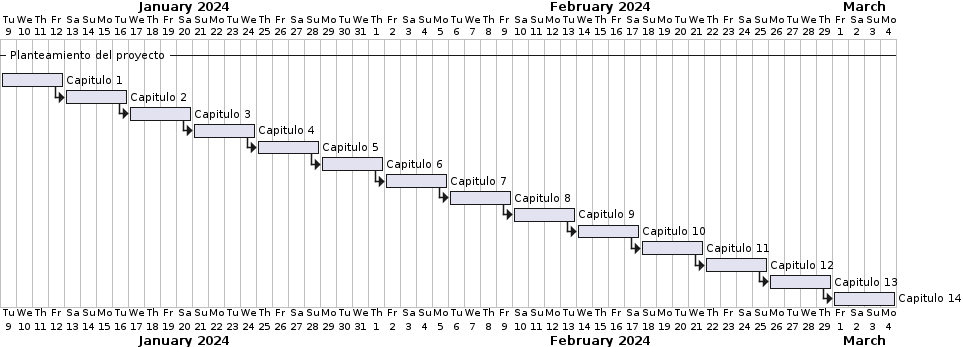
\includegraphics[width=1\linewidth]{figures/chapter01/Gantt.png}
    \caption{Diagrama Gantt}
    \label{fig:gantt}
\end{figure}
% TODO

\subsection{Presupuesto}

% TODO  


\section{Estructura de la memoria}

En este trabajo, hemos utilizado la documentación proporcionada por \textbf{PyTorch} para explicar diversos conceptos de las redes neuronales. Nos referimos a la documentación oficial de PyTorch \cite{pytorch2024github}. Usamos el término \texttt{torch}, \texttt{torch.nn} y \texttt{nn}.

% TODO
\clearpage\thispagestyle{empty}\cleardoublepage

\chapter{ANTECEDENTES Y ESTADO DEL ARTE}
\label{ch:2}
% ============================================================================================================== 
\section{Introducción}
\label{ch:2:section:introduction}

El proyecto que desarrollamos se encuentra en una frontera muy difusa de múltiples ramas del conocimiento, siendo muy interdisciplinar, se trata de una revisión de los ataques, seguridad y robustez a las redes neuronales centrandonos en ataques adversariales.
Por lo que debemos explicar que es la ciencia de datos, el proceso \gls{KDD}, la inteligencia artificial generativa y la seguridad informática.

\begin{figure}[H]
    \centering
    \centerline{\includesvg[width=0.75\columnwidth]{figures/ciencia-de-datos.drawio.svg}}
    \caption{Ciencia de datos como campo interdisciplinar.\\Fuente: Elaboración propia.}
    \label{fig:ciencia-de-datos}
\end{figure}

Podemos dividir este trabajo en dos secciones muy relacionadas, la primera la inteligencia artificial y de segundo punto de importancia la seguridad de la información.
Desde sus inicios la inteligencia artificial, aunque con buenos resultados en muchos campos de aplicación resultaba en grandes fallos de seguridad, fiabilidad y robustez.
Por cómo están entrenadas las inteligencias artificiales (\acrshort{ann}) tiene múltiples puntos de ataque que son susceptibles de ser atacados, los principales son los datos, las arquitecturas o los pesos.
Ya que alterando cualquiera de estos componentes de forma se verá enormemente afectada el comportamiento.

% Ciencia de la computación
% Mineria
% Machine Learning
% Deep Learning
% GANs

\section{Antecedentes}
\label{ch:2:section:background}

% region historia
\subsection{Historia, línea temporal}

A continuación se describe una línea de temporal con los hitos más relevantes en el desarrollo de las redes neuronales adjuntando con referencias las investigaciones, articulos y publicaciones realizadas.
En este caso se trata de referencias en hitos de logros a nivel teórico como práctico.

\begin{vtimeline}[timeline color=cyan!80!blue, add bottom line, line offset=2pt, use timeline header,timeline title={Hitos de las redes neuronales artificiales}]
    1676        & The Chain Rule \cite{leibniz2012early}                                                    \endlr
    1847        & Augustin-Louis Cauchy \cite{lemarechal2012cauchy}                                         \endlr
    1943        & Threshold Logic Unit (TLU) \cite{mcculloch1943logical}                                    \endlr
    1949        & Teoría Hebbiana                                                                           \endlr
    1958        & Perceptron \cite{rosenblatt1958perceptron}                                                \endlr
    1959-1960   & Adaline y Madaline \cite{rosenblatt1958perceptron}                                        \endlr
    1965        & Multilayer Perceptron (MLP) \cite{baum1988capabilities}                                   \endlr
    1967-1968   & Deep Learning by Stochastic Gradient Descent \cite{karplus19671967}                       \endlr
    1980’s      & Neuronas Sigmoidales                                                                      \endlr
    ~           & Feedforward neural network (FNN) \cite{rumelhart1985learning}                             \endlr
    ~           & Backpropagation (BP) \cite{rosenblatt1962principles,etde_5080493,lecun1985learning}       \endlr
    1985        & Boltzmann Machine \cite{ACKLEY1985147}                                                    \endlr
    1987        & Adaptive resonance theory (ART) \cite{grossberg1987competitive}                           \endlr
    1989        & Convolutional neural networks (CNN) \cite{lecun1989backpropagation}                       \endlr
    ~           & Recurent neural networks (RNN) \cite{schmidhuber1993habilitation}                         \endlr
    1990        & Generative Adversarial Networks (GAN) as Game \cite{schmidhuberunsupervised}              \endlr
    1997        & Long short term memory (LSTM) \cite{Hochreiter1997LongSM, hochreiter1997long}             \endlr
    2006        & Deep Belief Networks (DBN) \cite{hinton2006fast}                                          \endlr
    ~           & Restricted Boltzmann Machine \cite{hinton2006reducing}                                    \endlr
    ~           & Encoder / Decoder (Auto-encoder) \cite{hinton2006reducing}                                \endlr
    2014        & Generative Adversarial Networks (GAN) Moderns \cite{6294131,goodfellow2014generative}     \endlr
    2018        & Style Generative Adversarial Networks (Style-GAN) \cite{karras2019stylebased}             \endlr
\end{vtimeline}


\newpage
\subsection{Historia de la Inteligencia Artificial}

Todo surge en 1676 por {Gottfried Wilhelm Leibniz} \ref{fig:gottfried-leibniz} publicó la regla de la cadena del cálculo diferencial, esencial para el análisis matemático, es la esencial para calcular como cambiará la función final si se cambian los pesos de funciones anteriores.

La regla de la cadena es fundamental para técnicas como el descenso de gradiente, propuesto por {Augustin-Louis Cauchy} en 1847 y utilizado para ajustar iterativamente los pesos de una NN durante el entrenamiento.
Posteriormente en 1805 {Adrien-Marie Legendre} y {Johann Carl Friedrich Gauss} desarrollaron \acrshort{nn}, matemáticamente eran regresiones lineales muy simples, similares a las redes neuronales lineales simples.
Esto lo uso {Gauss} para redescubrir el planeta enano Ceres.

\begin{figure}[H]
    \centering
    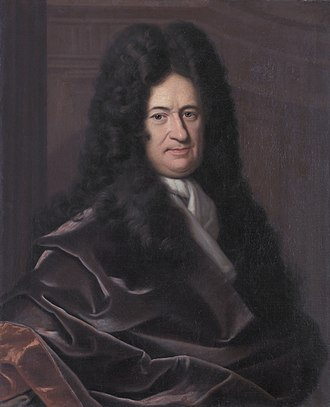
\includegraphics[width=0.45\textwidth]{figures/Gottfried_Wilhelm_Leibniz,_Bernhard_Christoph_Francke.jpg}
    \caption{Retrato de Gottfried Leibniz.\\Fuente: \href{https://es.wikipedia.org/wiki/Gottfried_Leibniz}{Wikipedia}}
    \label{fig:gottfried-leibniz}
\end{figure}

Aunque realmente la historia comienza en 1943 con la investigación de {Warren McCulloch} y {Walter Pitss}, publicaron el artículo \textit{A logical calculus of the ideas immanent in nervous activity} \cite{mcculloch1943logical}.
Dicho artículo creó distintas ramas de investigación (ordenadores digitales, inteligencia artificial, funcionamiento del perceptron).

\begin{figure}[H]
    \centering
    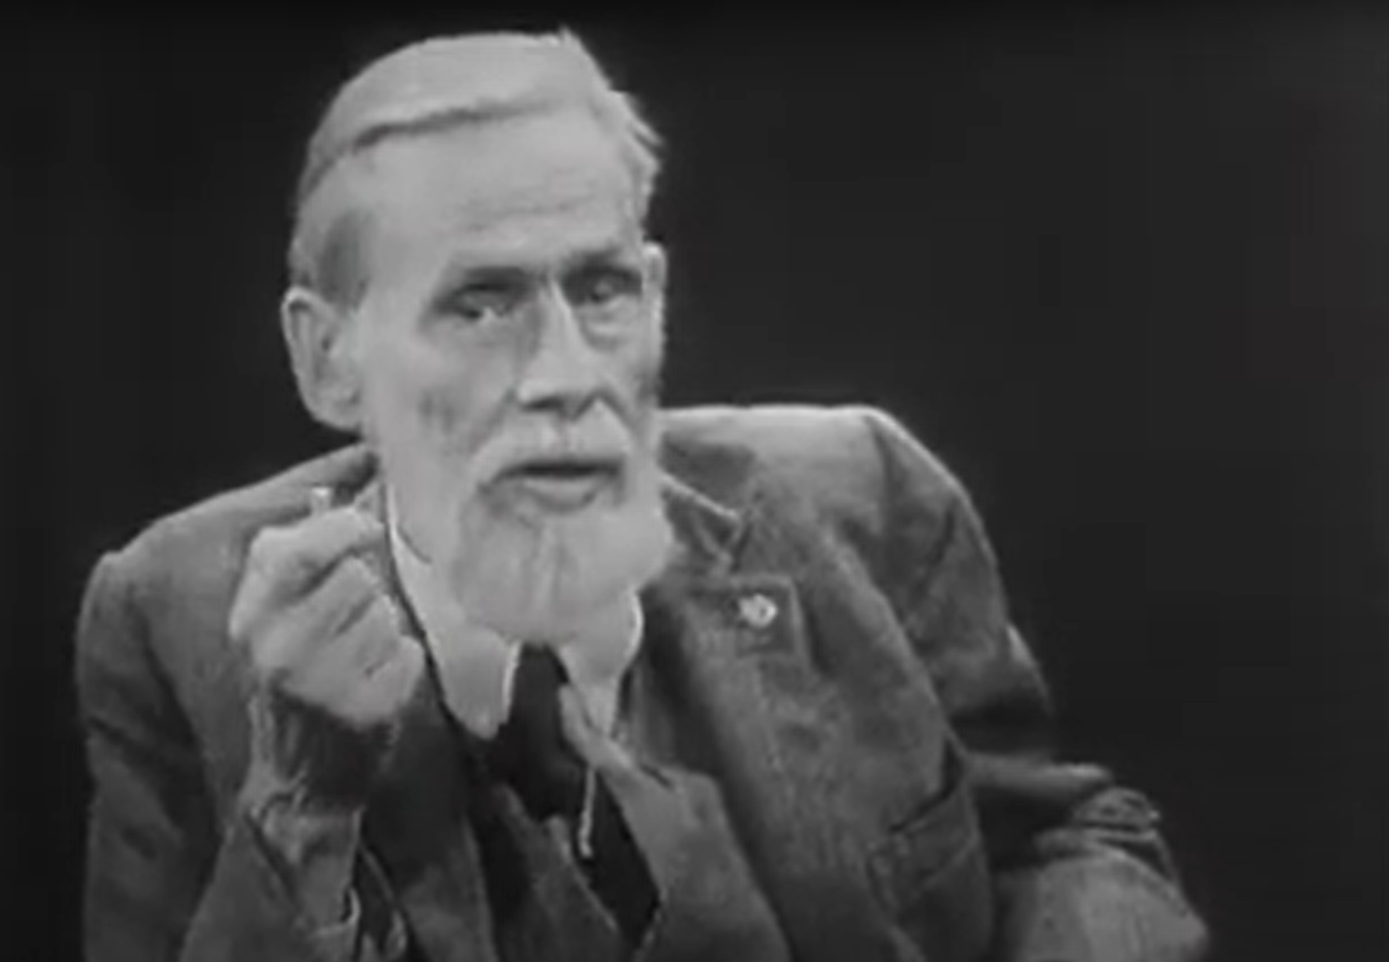
\includegraphics[width=0.65\textwidth]{figures/Warren Sturgis McCulloch Interview.png}
    \caption{Warren Sturgis McCulloch Interview.\\Fuente: \href{https://www.youtube.com/watch?v=8Wdz1Tj5084}{Entrevista en 1969}}
    \label{fig:Warren Sturgis McCulloch}
\end{figure}


En 1956 en la primera conferencia de inteligencia artificial organizada por la fundación {Rochester}, se reunen los investigadores fundadores de los conceptos actuales de la IA ({Minsky, McCarthy, Rochester, Shanon}), gran parte de la bibliografía se refiere a este punto como el origen y contacto de las redes neuronales artificiales.
En dicha conferencia (\textit{Nathaural Rochester}) presento el modelo de una red neuronal que fue el resultado de la investigación desarrollada por el equipo de investigación de IBM.

\begin{figure}[H]
    \centering
    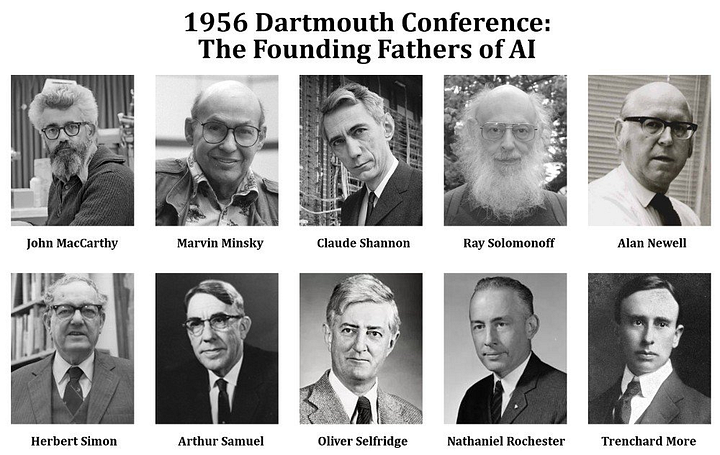
\includegraphics[width=0.75\textwidth]{figures/conferecia 1956 - 1689170718524.png}
    \caption{Los padres de la inteligencia artificial.\\Fuente: \href{https://www.linkedin.com/pulse/first-ever-ai-conference-tracing-evolution-history-ofai-nicky-verd}{Linkedin}}
    \label{fig:conferencia-1956}
\end{figure}

En 1957 se presenta el ``\textit{Perceptron}'' por {Frank Rosenblatt}, dicho elemento es un sistema clasificador de patrones, además contaba con la capacidad de aprender, de ser robusto matemáticamente y poder adaptarse si algún componente se dañaba.

\begin{figure}[H]
    \centering
    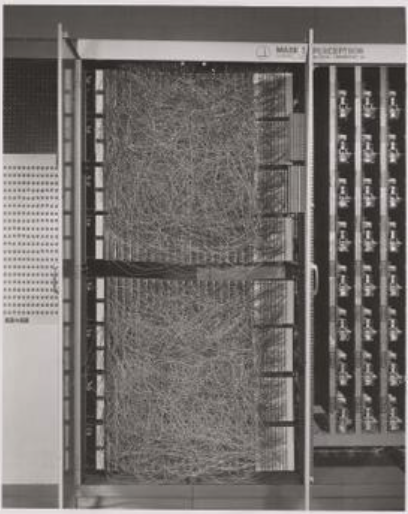
\includegraphics[width=0.4\textwidth]{figures/perceptron.png}
    \caption{Mark I Perceptron.\\Fuente: \href{https://en.wikipedia.org/wiki/Perceptron}{Wikipedia}}
    \label{fig:perceptron}
\end{figure}

El \textit{Perceptron} fue diseñado originalmente para el reconocimiento óptico usando un sistema de 400 fotocélulas en rejilla.
Posteriormente se describió el problema de no-linealidad que presentaban los perceptrones (Problema XOR) \cite{cuevastello2018apuntes}.

De 1959 a 1960 {Bernard Widrow} y {Ted Hoff} desarollaron ``Adaline'' y ``Madaline'' \cite{widrow1960adaptive} que resolvía el problema de la no-linealidad y que tenía aplicación en el reconocimiento de voz, series temporales, caracteres, etc.

Posteriormente el \textit{MIT} realizo una investigación matemática muy crítica de todos los problemas que presentaba el \textit{Perceptron} llegando a la conclusión que tenían grandes problemas que no podrían ser resueltos, por lo que en la próxima década (años 60) se redujo drásticamente las investigaciones sobre el campo de las redes neuronales.
Esto llevo a uno de los famosos inviernos de la inteligencia artificial (1974 - 1980).

\begin{figure}[H]
    \centering
    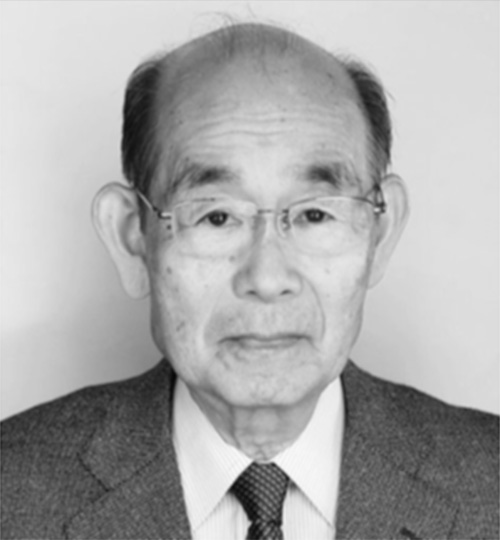
\includegraphics[width=0.25\textwidth]{figures/Kunihiko Fukushima.jpg}
    \caption{Kunihiko Fukushima.\\Fuente: \href{https://www.ieice.org/eng/about_ieice/new_honorary_members_award_winners/2017/meiyo_05e.html}{IEICE}}
    \label{fig:kunihiko-fukushima}
\end{figure}

Durante la década de los 70 se hacen aportes a la teoría \textit{Hebbiana}, se aportan logros en al análisis y descripción de reglas adaptativas, además de otros aportes al principio de aprendizaje competitivo.
En 1979 presentó {Kunihiko Fukushima} la primera red neuronal \acrshort{cnn}, la llamó Neocognitron \cite{fukushima1979neural}, dicho trabajo en un futuro se mejoraría con técnicas de \gls{BP-NN}.

En la década de los 80 se realizaron aportes como el algoritmo de \gls{BP-NN} que surgio del artículo de {Hopfield} \cite{hopfield1982neural}, esto despertó la curiosidad de muchos investigadores a volver al campo de las redes neuronales.
Se realizaron aportes como las redes \acrshort{gnn}.
La investigación continuó con {Stephen Grossberg} que realizo aportes derivados de estudios fisiológicos de cómo funcionaban las neuronas y la plasticidad, lo que permitió la creación de reglas y postulados, esto se ve en los trabajos de las redes \acrshort{art-nn} \cite{grossberg1987competitive}.
La investigación de {Hopfield} basada en el trabajo de {Stephen Grossberg} creo un sistema computacional neuronal interconectado que tiende a un mínimo de energía.
En 1985 {David E. Rumelhart} basandose en la investigación realizada por {Paul Werbos} \cite{etde_5080493} realizo un análisis experimental del algoritmo \gls{BP-NN} y su aplicación en redes \acrshort{fnn} \cite{rumelhart1985learning}.

{Yann LeCun} junto a su equipo, en 1989 crearon la primera aplicación \acrshort{cnn} con técnicas \acrshort{bp} dicha aplicación podía reconocer números a partir de imágenes.

\begin{figure}[H]
    \centering
    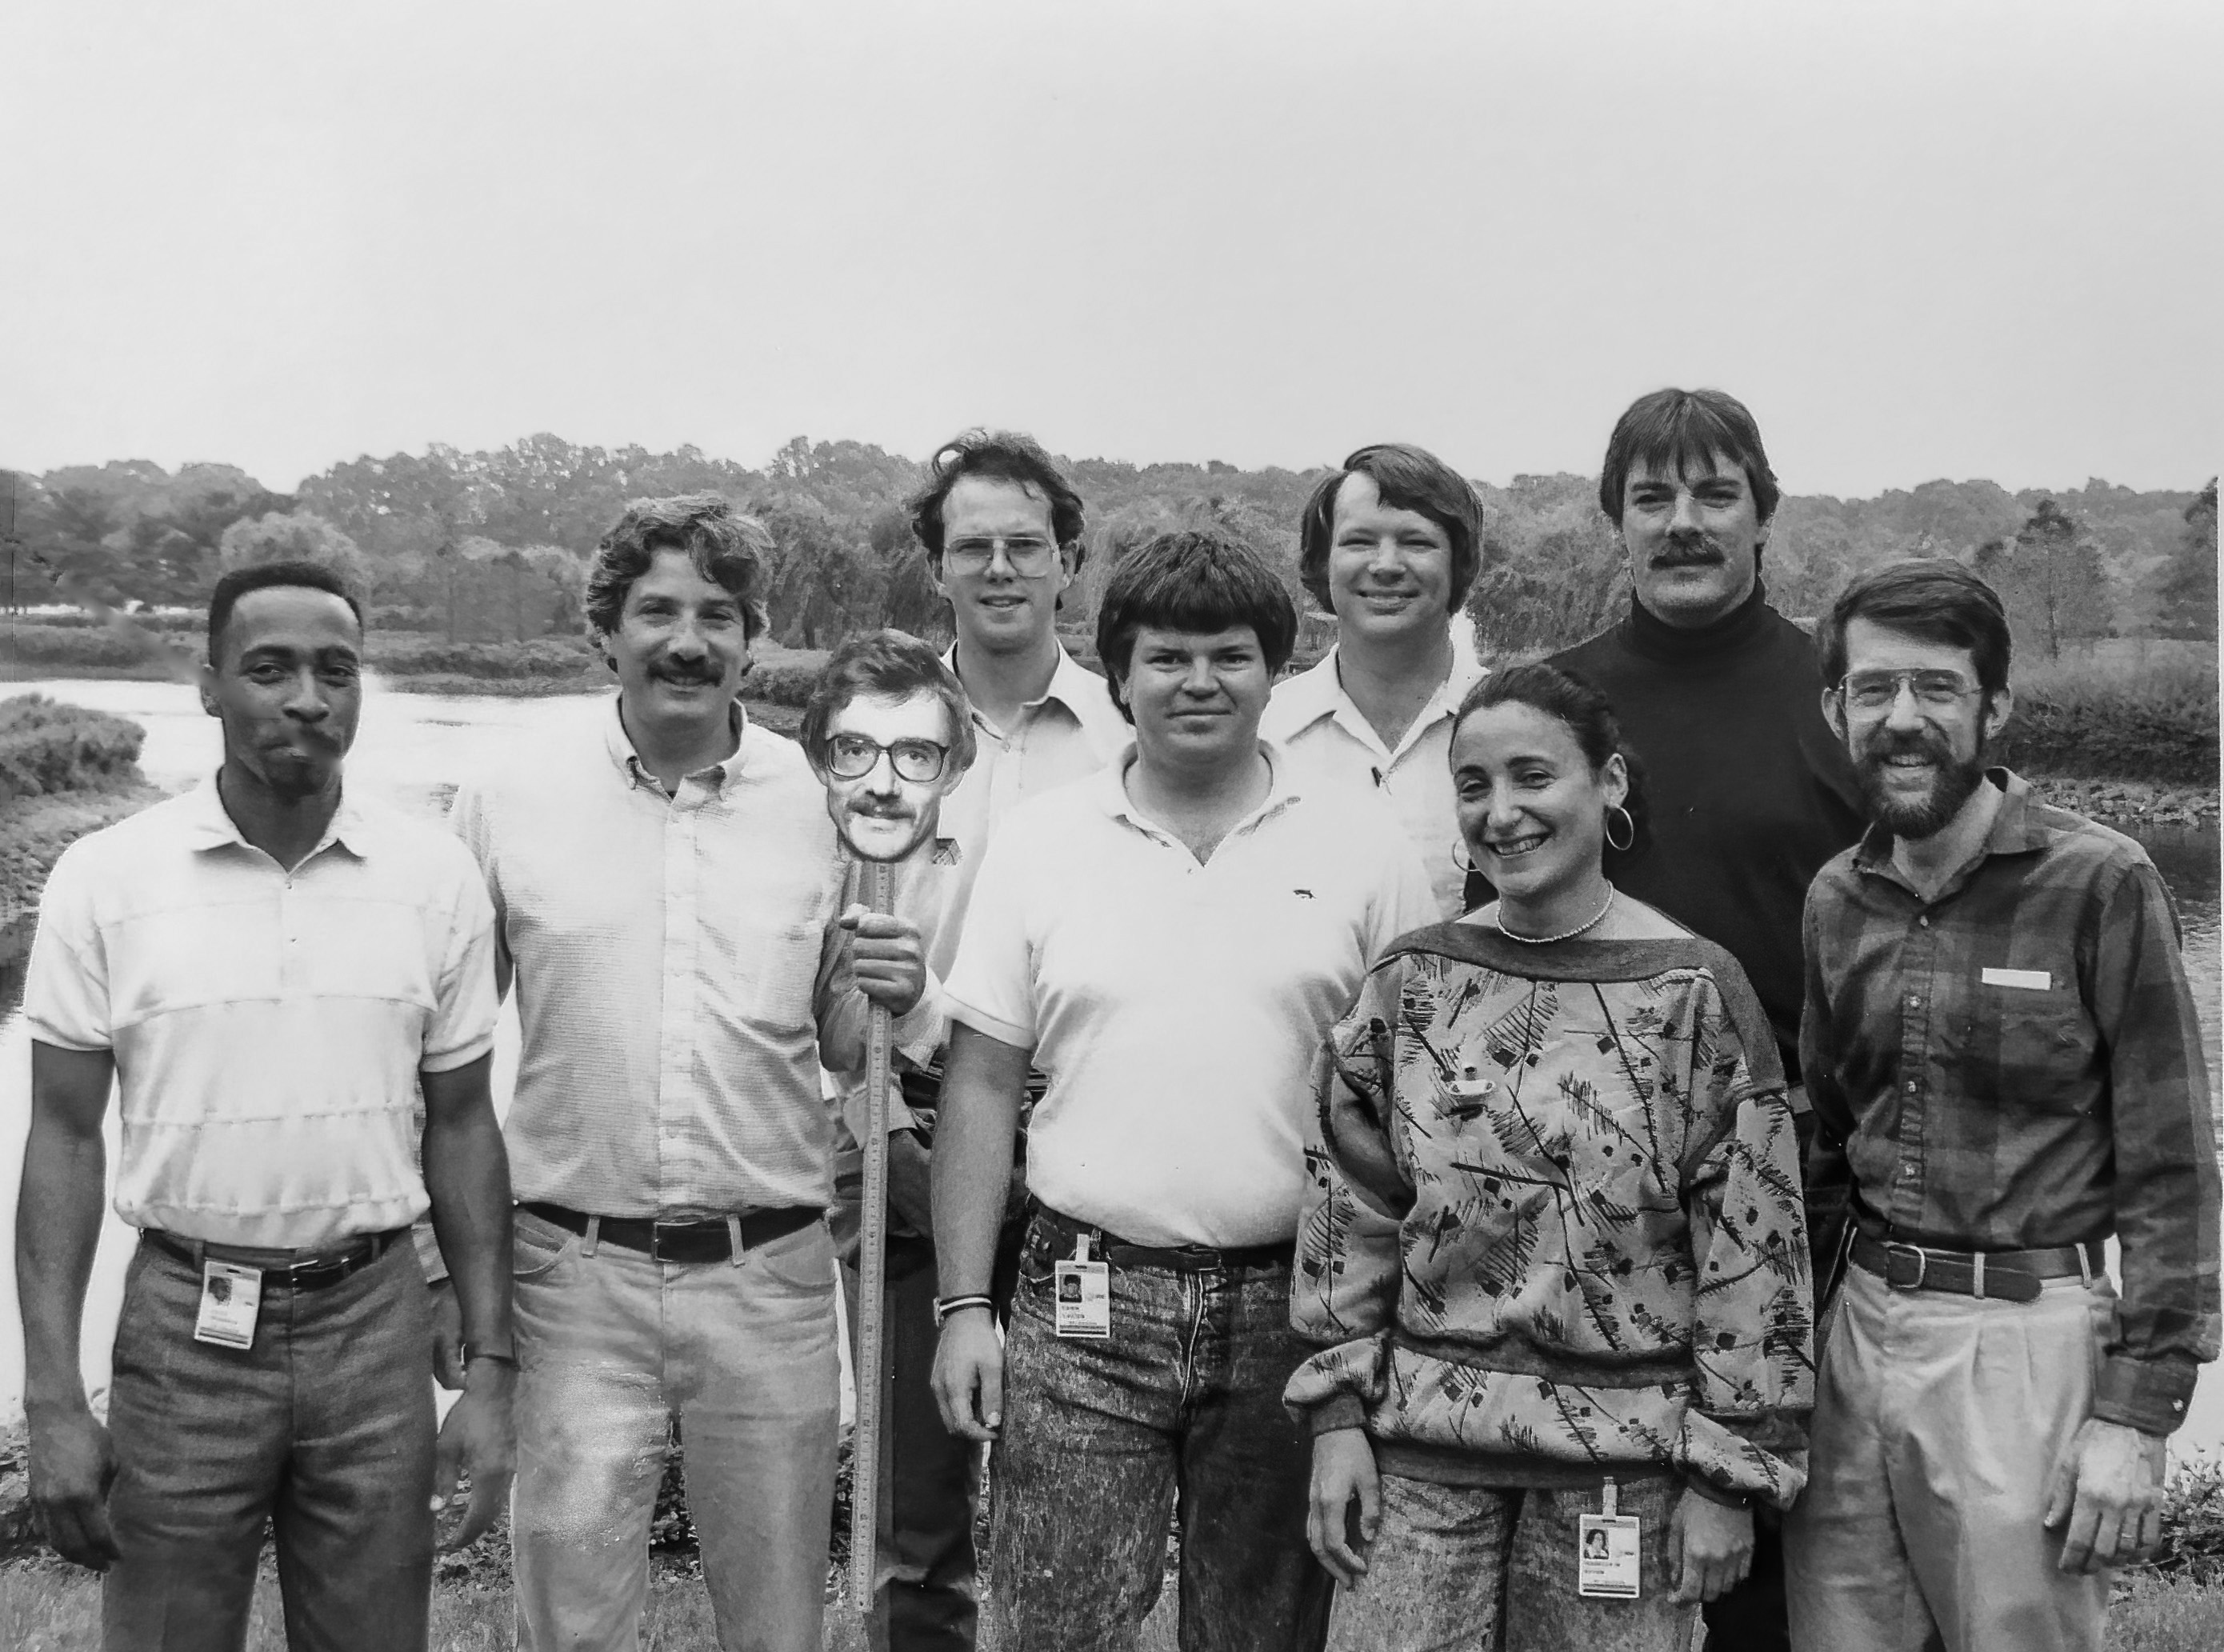
\includegraphics[width=0.65\textwidth]{figures/yann-lecun - EyIwmEDW8AIQs1C.jpeg}
    \caption{Adaptive Systems Research Department at Bell Labs 1989.\\Fuente: \href{https://twitter.com/ylecun/status/1378718317695934465}{Twitter Yann Lecun}}
    \label{fig:adaptive-systems-research-department-at-bell-labs}
\end{figure}

En la década de los 90 se presentaron múltiples investigaciones y muchos avances en el campo, uno de los más importantes fue la presentación de la primera \acrshort{gan} como una curiosidad, ya que se presentó como un duelo entre dos redes neuronales, en un principio fue un generador probabilístico y un predictor con el objetivo de maximizar la pérdida de cada uno en un juego \textit{minimax}.

En 1991 se presentó el trabajo \textit{Predictability Minimization} \cite{urgen1991learning} dichas técnicas sirvieron de inspiración para el aprendizaje por refuerzo,
En marzo de 1991 se hizo una aproximación a los \textit{transformers} con auto atención, lograron separar el conocimiento del control como una máquina clásica, pero de una forma completamente neuronal, además de gestionar actualizaciones de los pesos de forma muy rápida y eficiente.

Durante la década de 1990 las redes neuronales tendían a ser muy sencillas, con pocas capas y no muy complejas por las limitaciones técnicas de la época.
Por lo que muchos investigadores propusieron soluciones similares a las redes \acrshort{rnn} que permitían una retroalimentación, además de aceptar secuencias de información arbitraria.
Otros propusieron soluciones como la jerarquía de \acrshort{rnn} autosupervisada que aprende representaciones en distintos niveles de abstracción.
Comienzan a proponerse redes similares a las que en un futuro se llamarían \acrshort{dbn} como un método no supervisado para \acrshort{fnn}.

En junio de 1991 {Sepp Hochreiter} Figura \ref{fig:sepp-hochreiter} implemento el primer compresor de redes neuronales, además demostró uno de los principales problemas de las \acrshort{nn} el llamado problema del desvanecimiento o explosión del gradiente \ref{gradient-descent} que hacía que el aprendizaje fallará.
Un análisis posterior condujo a los investigadores a una primera aproximación \acrshort{lstm}, aunque no sería hasta 1997 con la revisión por pares y publicación del artículo \textit{Long short-term memory} \cite{hochreiter1997long} que se solucionaría parcialmente el problema.

\begin{figure}[H]
    \centering
    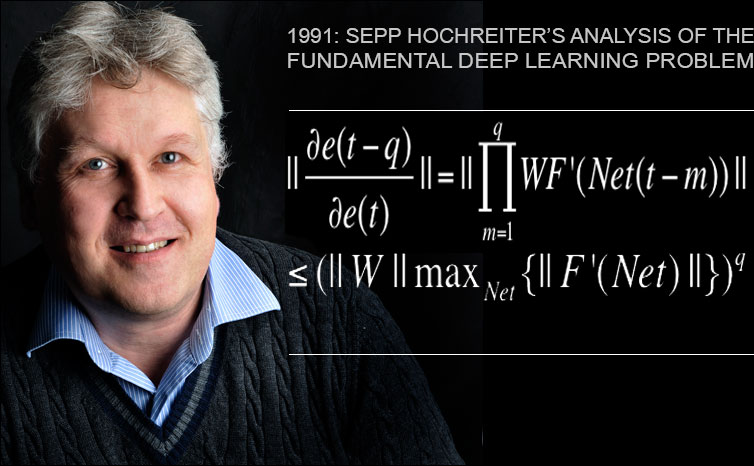
\includegraphics[width=0.65\textwidth]{figures/Sepp Hochreiter.jpg}
    \caption{Sepp Hochreiter.\\Fuente: \href{https://people.idsia.ch/~juergen/fundamentaldeeplearningproblem.html}{IDSIA}}
    \label{fig:sepp-hochreiter}
\end{figure}

Más adelante en el 2014 {Goodfellow} Figura \ref{fig:gan-ian-goodfellow} presento la primera red neuronal \acrshort{gan} pura para la generación de imágenes mediante el enfrentamiento de una red neuronal generativa contra una red neuronal discriminante entrenadas con el mismo conjunto de datos \cite{goodfellow2014generative}.
Durante los próximos años se realizaron muchos aportes a las redes neuronales generativas, principalmente de paralelización de los cálculos, técnicas de estabilización, generación condiciona, arquitecturas más eficientes, funciones de pérdidas más adecuadas, aplicaciones específicas (cambiar el estilo de pintura), redes apiladas, etc.
Fruto de todo ello {NVIDIA} en 2018 presento \gls{StyleGAN} \cite{karras2019stylebased} aunque publicaron el código en 2019 con fuertes mejoras.

\begin{figure}[H]
    \centering
    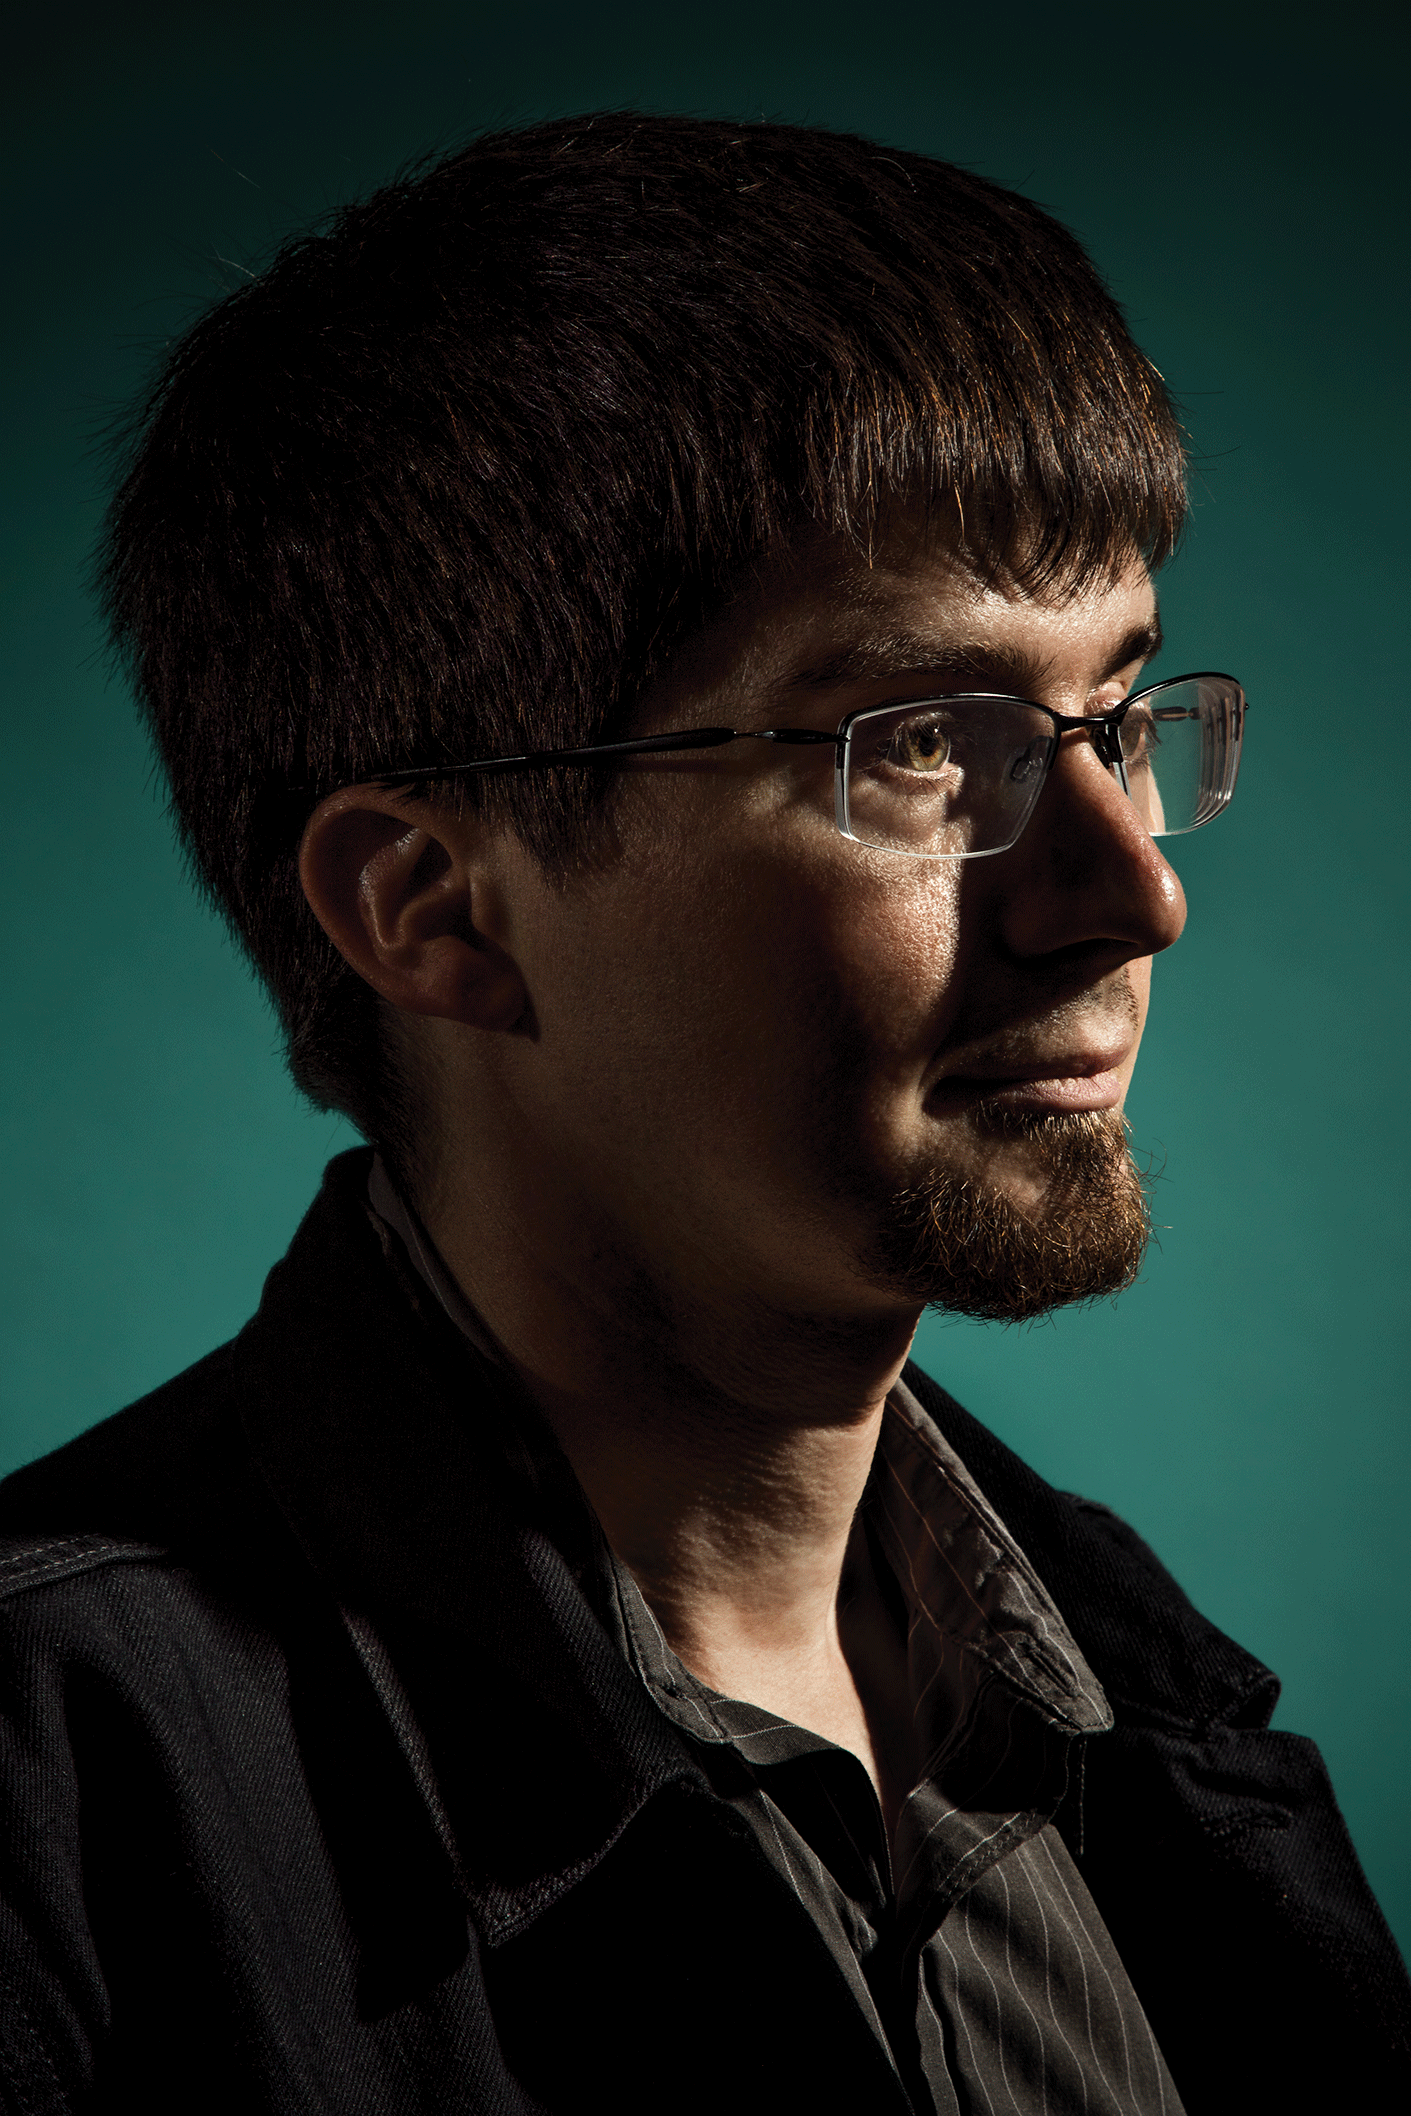
\includegraphics[width=0.2\textwidth]{figures/gan-goodfellow.png}
    \caption{Ian Goodfellow.\\Fuente: \href{https://www.technologyreview.es/s/10016/el-senor-de-las-gan-el-hombre-que-dio-imaginacion-las-maquinas}{MIT Technology Review}}
    \label{fig:gan-ian-goodfellow}
\end{figure}
% endregion


\section{Estado del arte}
\label{ch:2:section:state-of-the-art}

% region Teoría
\subsection{La ciencia de datos}
La ciencia de datos (\textit{Data Science}) es el estudio de los datos con el objetivo de extraer información útil, se usa principalmente para dar información útil a empresas. Es un campo multidisciplinar, ya que combina campos de las matemáticas, estadistica e inteligencia artificial para analizar grandes cantidades de datos. Esto tiene como objetivo responder a las siguientes cuestiones: \textit{¿Qué paso?, ¿Por qué pasó?, ¿Qué pasará? o ¿Qué se puede hacer con los resultados?} \cite{aws-data-science}

La ciencia de datos analiza los datos de distintas formas.

\begin{enumerate}
    \item \textbf{Análisis descriptivo}: examina datos con visualizaciones (gráficos, tablas) para entender eventos pasados o actuales.
    \item \textbf{Análisis de diagnóstico}: profundiza en los datos para entender las razones detrás del evento. Emplea técnicas cómo descubrimiento de datos o correlaciones.
    \item \textbf{Análisis predictivo}: utiliza datos históricos y técnicas como machine learning para hacer predicciones precisas sobre patrones futuros.
    \item \textbf{Análisis prescriptivo}: busca la mejor respuesta para un resultado esperado. Utiliza técnicas como simulación y redes neuronales para recomendar el mejor curso de acción entre varias alternativas.
\end{enumerate}


\subsection{La mineria de datos}
% Fases de la extraccón del conocimiento 
% Dentro del KDD está la {Mineria de datos}

La minería de datos, es una técnica asistida por computadora, procesa grandes conjuntos de datos para descubrir patrones y relaciones ocultas. Este conocimiento resultante se aplica en la resolución de problemas, análisis de decisiones empresariales, etc. Esta técnica tiene distintas fases para procesar y extraer información útil.

\begin{enumerate}
    \item Comprender, identificar y definir el alcance del proyecto.
    \item Comprender los datos.
    \item Depurar datos (limpiar, integrar y dar formato).
    \item Modelar datos.
    \item Evaluar los resultados.
    \item Implementar resultados.
\end{enumerate}

La mineria de datos es distinta en función de los datos y el objetivo, la mayoria del estado del arte segmenta la mineria en tres tipos, mineria de procesos, mineria de textos y mineria predictiva.

El Descubrimiento de Conocimientos en Bases de Datos \gls{KDD} es un proceso que utiliza algoritmos de minería de datos para explorar y extraer conocimientos útiles de grandes bases de datos. Con el avance tecnológico, se emplean técnicas de inteligencia artificial para este propósito, con el objetivo final de obtener conocimiento de alto nivel a partir de datos de bajo nivel. La Figura \ref{fig:kdd} esquematiza el proceso general del \textit{KDD}.

\begin{figure}[H]
    \centering
    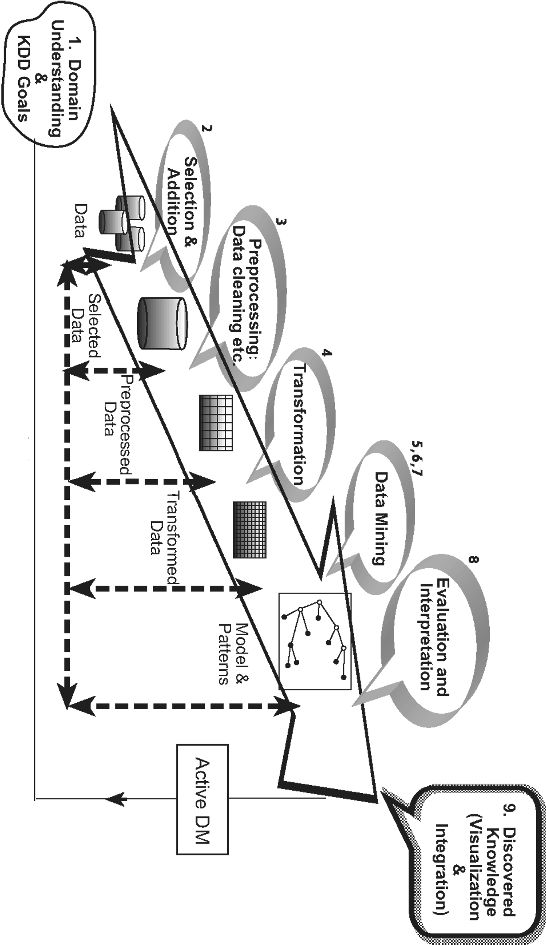
\includegraphics[angle=90,width=0.8\textwidth]{figures/chapter02/KDD.jpg}
    \caption{El proceso de descubrimiento de conocimiento en bases de datos.\\Fuente: Sección \textit{Introduction to Knowledge Discovery and Data Mining} \cite{rokach2010data}}
    \label{fig:kdd}
\end{figure}


\begin{enumerate}
    \item \textbf{Comprensión del Dominio de Aplicación}: se debe comprender los datos que se tratan y el campo de obtención con el objetivo de preparar los datos.
    \item \textbf{Selección y Creación de Conjunto de Datos}: se han de seleccionar los datos relevates (Selección de características).
    \item \textbf{Preprocesamiento y Limpieza de Datos}: se han de eliminar las características no relevantes, datos perturbados, entradas incoherentes o tratar datos faltantes, etc. con el objetivo de obtener datos más limpio.
    \item \textbf{Transformación de Datos}: se deben tratar los datos, reduciendo la dimensionalidad, filtración, descomponiendo, etc. para que sea más sencillo el consumo de estos datos por una aplicación.
    \item \textbf{Elección de Tarea de Minería de Datos}: en función de los datos y del objetivo deberemos realizar una tarea (clasificación, regresión o agrupación), ya que en la mineria de datos hay dos objetivos principales, \textbf{predicción} y \textbf{descripción}.
    \item \textbf{Elección del Algoritmo de Minería de Datos}: deberemos elegir entre los distintos algoritmos que se usan en la mineria de datos, si buscamos precisión podemos usar redes neuronales, si buscamos explicabilidad podemos usar arboles de decisión.
    \item \textbf{Implementación del Algoritmo de Minería de Datos}: emplearemos el algoritmo seleccionado ajustando las parámetros para que nos de el mejor resultado.
    \item \textbf{Evaluación de Patrones Minados}: debemos interpretar los resultados (reglas, confiabilidad, etc) si no cumplen los objetivos que se buscaban en el primer paso deberemos reajustar toda la metodologia, desde ajustar la selección de características a la interpretación o compresibilidad del modelo.
    \item \textbf{Utilización del Conocimiento Descubierto}: por último debemos incorporar el conocimiento a los sistemas de toma de decisiones, este es el paso más importante, ya que con el podemos medir los efectos del conocimiento obtenido. Puede suceder que una vez implementado el modelo en sistema de producción pierda eficiencia si las condiciones reales son distintas a las de la creación del modelo.
\end{enumerate}


\begin{figure}[H]
    \centering
    \centerline{\includesvg[width=1\linewidth]{figures/chapter02/data-mining-taxonomy.drawio.svg}}
    \caption{Taxonomía de minería de datos.\\Fuente: Elaboración propia, inspirado en la sección \textit{Introduction to Knowledge Discovery and Data Mining} \cite{maimon2005data}}
    \label{fig:data-mining-taxonomy}
\end{figure}

La mineria de datos puede estár orientada a la verificación o al descubrimiento de patrones, se debe automatizar su identificación, puediendo usar un efoque predictictivo o descriptivo. Para el descubrimiento se usa el aprendijaze inductivo, mientras que en la verificación se ha de evaluar la hipótesis externas usando métodos estádisticos clásicos. La terminología clásica del aprendizaje automatico está clasificado en supervisado (clasificación y regresión) y no supervisado (agrupamiento), aunque existen muchos más términos en la terminología moderna esto podemos analizarlo más en profundidad en el libro \textit{Data Mining and Knowledge Discovery Handbook} \cite{maimon2005data}.


\subsection{Aprendizaje automático - \textit{Machine Learning}}

El \textit{machine learning} es la ciencia o rama de la inteligencia artificial que desarrolla, modelos estadisticos, desarrolla algoritmos que generalizan comportamientos y reconocen patrones. Es decir hace posible el aprendijaze autónomo de las máquinas para realizar tareas sin la necesidad programar las instrucciones explícitamente. El \textit{machine learning} busca procesar grandes cantidades de datos e identificar patrones de datos de forma automática.

\begin{figure}[H]
    \centering
    \centerline{\includesvg[width=0.75\linewidth]{figures/chapter02/machine-learning-rules.drawio.svg}}
    \caption{El \textit{Machine Learning} como paradigma de programación.\newline{}Fuente: Elaboración propia.}
    \label{fig:machine-learning-rules}
\end{figure}

Como podemos ver en la Figura \ref{fig:machine-learning-rules} en el paradigma clásico se necesitaba conocer el dominio de los datos y las reglas en profundidad y programar los descriptores de forma manual para procesar los datos. En el paradigma del \textit{machine learning} permite extraer esas reglas y patrones para procesar nuevos datos a partir de respuestas que conociamos previamente, estas respuestas previas deben ser extraidas o validadas por expertos.

Una clásificación de las tareas del \textit{machine learning} lo podemos ver en la Figura \ref{fig:machine-learning}, esta clasificación está dividida en función de como se realiza el aprendijaze del modelo.

\begin{figure}[H]
    \centering
    \centerline{\includesvg[width=1\linewidth]{figures/chapter02/machine-learning.drawio.svg}}
    \caption{Clasificación de los algoritmos de aprendijaze automático.\\Fuente: Elaboración propia.}
    \label{fig:machine-learning}
\end{figure}

El \textit{machine learning} puede trabajar con datos estructurados y no estructurados aunque estos últimos requieren un procesamiento previo para adapatarlos en un formato estructurado.



\subsection{Aprendizaje profundo - \textit{Deep Learning}}
% TODO: Explicar el Deep Learning https://idus.us.es/bitstream/handle/11441/90004/Centeno%20Franco%20Alba%20TFG.pdf

El \textit{deep learning} es una subrama del \textit{machine learning} que usa redes neuronales artificiales para analizar datos no lineales, estas redes imitan el comportamiento del cerebro humano, para esto suelen contar con arquitecturas complejas.
Se distingue del \textit{machine learning} por los tipos de datos con los que puede trabajar y por los métodos con los que hace que los modelos aprendan.

Otra de las carácteristicas que diferencia al \textit{deep learning} del \textit{machine learning} es que elimina parte del procesamiento previo de datos, ya que sus algoritmos puede ingerir y procesar datos no estructurados.


%  ============================================================================================================================================================
%  ============================================================================================================================================================
%  ============================================================================================================================================================

\subsection{Redes neuronales artificiales - \textit{Artificial Neuronal Networks}}
% TODO: \cite{ibm-deep-learning}
% Explicar uso de multiples neuronas artificiales para crear capas y luego redes
El \textit{deep learning} emplea principalmente redes neuronales para reconocer, clasificar y describir con precisión patrones de datos. Estas redes están inspiradas en el funcionamiento del cerebro humano.  \cite{ibm-deep-learning}

Las redes neuronales es un conjunto de neuronas artificiales que están organizadas generalmente por capas. Estas redes tienen una capa de entrada, una capa de salida y multiples capas ocultas con distintas funciones de activación que ponderan los pesos de cada neurona.

Existen formas muy variadas de componer las capas, a esto se le denomina \textbf{topologia de red neuronal}, en función del objetivo que se busque, la topologia será muy distinta.

\subsubsection{Elementos de una neurona artificial}

Como se ha comentado previamente las neuronas artificiales están inspiradas en las neuronas biologicas del cerebro humanos, fueron los investigadores \textit{McCulloch} y \textit{Pitts} \cite{mcculloch1943logical} los que sentaron las bases de lo que es una neurona artificial, demostrando que su modelo de red neuronal podía realizar cálculos que se correspondían con la lógica proposicional.

% TODO explicar las partes que propusieron \textit{McCulloch} y \textit{Pitts} 

\begin{figure}[H]
    \centering
    \centerline{\includesvg[width=1\linewidth]{figures/chapter02/artificial-neuron.drawio.svg}}
    \caption{Partes de una neurona artificial bioinspirada en una neurona biológica.\\Fuente: Elaboración propia}
    \label{fig:artificial-neuron}
\end{figure}

En la Figura \ref{fig:artificial-neuron} podemos ver las distintas partes de una única neurona artificial y sus partes equivalentes con una neurona biológica. El axón opera como la entrada de información a la neurona,

% Perceptron
%% LTU 

% Perceptron simple: %% solo dos capas, la red es unidireccional, la primera capa no realiza calculos, solo consume los datos de entrada, la segunda capa unicamente aplica una f. de activación de paso o signo 
% Perceptrón múltiple

\subsubsection{Funcionamiento de una red neuronal \label{neural-network}}

Las redes neuronales profundas tienen multitud de capas con nodos interconectados, cada capa sobre la capa anterior con el objetivo de optimizar la precisión de una predición o clasificación. A esta progresión de calculos se le denomina ``propagación hacia delante''.

El proceso de ``propagación inversa'' es el encargado de calcular errores de precisión, ajustar sesgos y ponderaciones usando algoritmos como el descenso de gradiente.

% TODO: Fases por la que se pasa una red neuronal

La capa de entrada es por donde el modelo ingiere los datos, y la capa de salida es donde el modelo responderá con la predicción o clasificación una vez se haya completado la fase de aprendizaje.

\begin{figure}[H]
    \centering
    \centerline{\includesvg[width=1\linewidth]{figures/chapter02/neuronal-network.drawio.svg}}
    \caption{Red neuronal artificial.\\Fuente: Elaboración propia}
    \label{fig:artificial-neuronal-network}
\end{figure}

En la Figura \ref{fig:artificial-neuronal-network} podemos ver una arquitectura simple de una red neuronal que cuenta con la capa de entrada, la capa de salida y dos capas ocultas.

El vector de entrada $X = (x_{1}, x_{2}, ..., x_{n})$ será la información suministrada a nuestra red a través de la capa de entrada, este vector será de tamaño $n$.


\begin{figure}[H]
    \centering
    \centerline{\includesvg[width=1\linewidth]{figures/equations/Notation.drawio.svg}}
    \caption{Calculo de los pesos de la red neuronal artificial.\\Fuente: Elaboración propia}
    \label{fig:notation}
\end{figure}

\begin{enumerate}
    \item Función de la red neuronal: $f(x) = W x + b$
    \item Matriz de pesos: $W = \left[w_{0,n}, w_{1,n}, ...,w_{m,n}\right]$
    \item Vector de pesos: $w_{n} \in \mathbb{R}^{D}$
    \item Vector de entrada: $x \in \mathbb{R}^{D}$
    \item Vector del bias: $b \in \mathbb{R}^{C}$
\end{enumerate}

% El proceso de reducción de dimensionalidad se lleva a cabo, para convertir el vector de características del espacio original en un nuevo espacio con un conjunto más pequeño, linealmente no correlacionadas mediante la siguiente función $f: \mathbb{R}^{D} \rightarrow \mathbb{R}^{C}$ con $C \ll D$, donde la red neuronal está expresada como $f(x) = W x + b$. Está red cuenta con las siguientes partes $\mathbf{W} = \left[w_{0}^{T}, w_{1}^{T}, ..., w_{C}^{T}\right]$ es la matriz de vectores de peso, que viene dada la expresión $\mathbf{w_{j}} \in \mathbb{R}^{D}$. El vector de entrada es $\mathbf{x} \in \mathbb{R}^{D}$ y el $bias$ es un vector que está definido en el espacio $\mathbf{b} \in \mathbb{R}^{C}$

\paragraph*{El perceptron simple}
\paragraph*{El perceptron multicapa}


% Multicapa
% Funciones de optimización
% Funciones de activación
% Funciones de perdida
% Capas
% Topologias
% Descenso de gradiente



\subsubsection{Funciones de activación}
% region Funciones de activación
% TODO: definición, explicación y tipos, solo mostramos las más importantes
Existen muchas funciones de acttivación que modifican las neuronas


\paragraph*{\textit{Non-linear Activations (weighted sum, nonlinearity)} \cite{pytorch2024github}}

\begin{enumerate}
    \item \textbf{ReLU}:
    \item[] \begin{equation} \varphi(x) = \operatorname*{max}(0,x) \end{equation}
    \item \textbf{LeakyReLU}:
    \item[] \begin{equation} \varphi(x) = \operatorname*{max}\left(0,x\right) + \operatorname*{negative\_slope} * \operatorname*{min}\left(0,x\right)  \end{equation}

    \item \textbf{Softplus}:
    \item[] \begin{equation} \varphi(x) = \frac{1}{\beta} \operatorname*{log}\left(1+e^{\beta x}\right) \end{equation}
    \item \textbf{SoftSign}:
    \item[] \begin{equation} \varphi(x) = \frac{x}{1+\lvert x \rvert} \end{equation}

    \item \textbf{Tanh}:
    \item[] \begin{equation} \varphi(x) = \frac{e^{x}-e^{-x}}{e^{x}+e^{-x}} \end{equation}
    \item \textbf{Sigmoid}:
    \item[] \begin{equation} \varphi(x) = \frac{1}{1+e^{-x}} \end{equation}
\end{enumerate}

\begin{figure}[H]
    \centering
    \captionsetup{justification=centering}

    \begin{subfigure}{.475\linewidth}
        \centering
        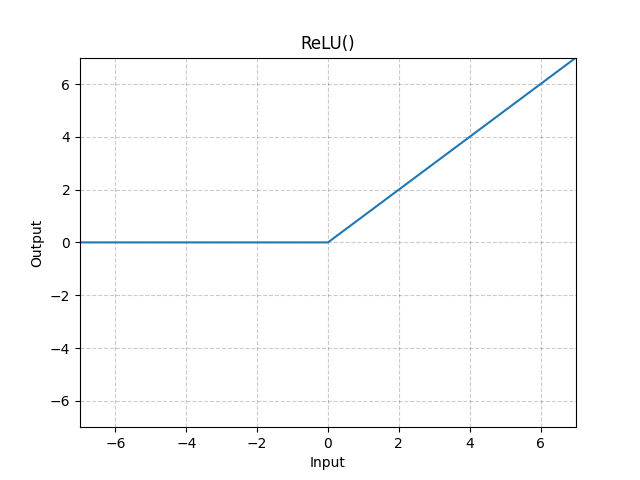
\includegraphics[width=0.75\linewidth]{figures/equations/ReLU.png}
        \caption{Función de activación ReLU.\newline{}Fuente: \href{https://pytorch.org/docs/stable/generated/torch.nn.ReLU.html}{Pytorch torch.nn.ReLU}}
        \label{subfig:torch.nn.ReLU}
    \end{subfigure}\hfill % <-- "\hfill"
    \begin{subfigure}{.475\linewidth}
        \centering
        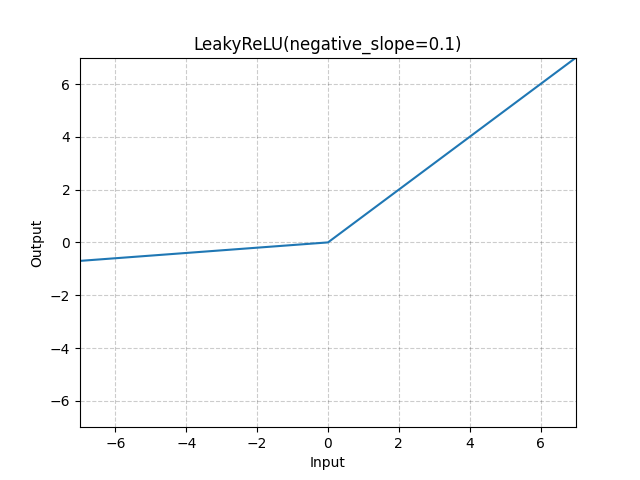
\includegraphics[width=0.75\linewidth]{figures/equations/LeakyReLU.png}
        \caption{Función de activación LeakyReLU.\newline{}Fuente: \href{https://pytorch.org/docs/stable/generated/torch.nn.LeakyReLU.html}{Pytorch torch.nn.LeakyReLU}}
        \label{subfig:torch.nn.LeakyReLU}
    \end{subfigure}

    \medskip % create some *vertical* separation between the graphs
    \begin{subfigure}{.475\linewidth}
        \centering
        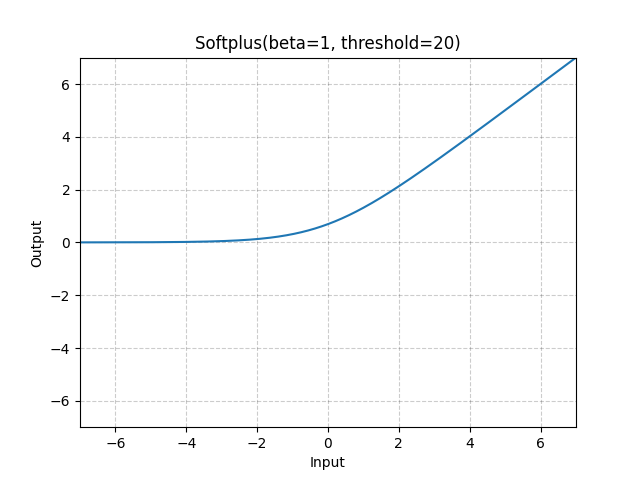
\includegraphics[width=0.75\linewidth]{figures/equations/Softplus.png}
        \caption{Función de activación Softplus.\newline{}Fuente: \href{https://pytorch.org/docs/stable/generated/torch.nn.Softplus.html}{Pytorch torch.nn.Softplus}}
        \label{subfig:torch.nn.Softplus}
    \end{subfigure}\hfill % <-- "\hfill"
    \begin{subfigure}{.475\linewidth}
        \centering
        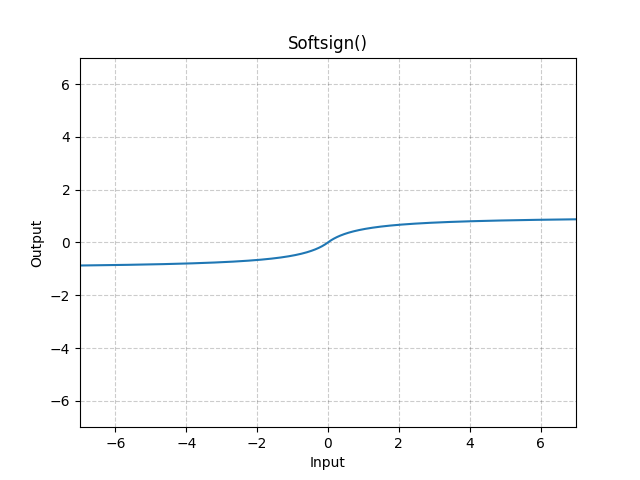
\includegraphics[width=0.75\linewidth]{figures/equations/Softsign.png}
        \caption{Función de activación Softsign.\newline{}Fuente: \href{https://pytorch.org/docs/stable/generated/torch.nn.Softsign.html}{Pytorch torch.nn.Softsign}}
        \label{subfig:torch.nn.Softsign}
    \end{subfigure}

    \medskip % create some *vertical* separation between the graphs
    \begin{subfigure}{.475\linewidth}
        \centering
        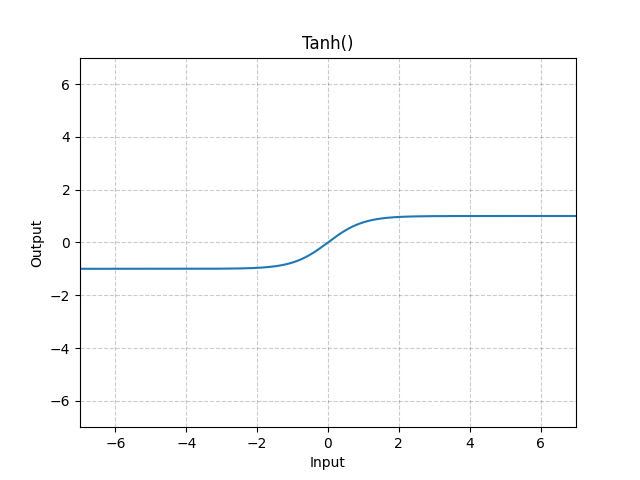
\includegraphics[width=0.75\linewidth]{figures/equations/Tanh.png}
        \caption{Función de activación Tanh.\newline{}Fuente: \href{https://pytorch.org/docs/stable/generated/torch.nn.Tanh.html}{Pytorch torch.nn.Tanh}}
        \label{subfig:torch.nn.Tanh}
    \end{subfigure}\hfill % <-- "\hfill"
    \begin{subfigure}{.475\linewidth}
        \centering
        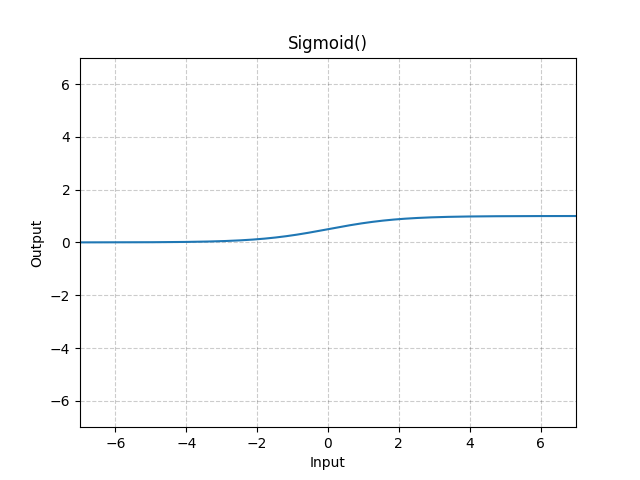
\includegraphics[width=0.75\linewidth]{figures/equations/Sigmoid.png}
        \caption{Función de activación Sigmoid.\newline{}Fuente: \href{https://pytorch.org/docs/stable/generated/torch.nn.Sigmoid.html}{Pytorch torch.nn.Sigmoid}}
        \label{subfig:torch.nn.Sigmoid}
    \end{subfigure}

    \caption{Funciones de activación no lineales}
    \label{fig:equations--Non-linear-Activations}
\end{figure}


\subparagraph{\textit{Non-linear Activations (other)} \cite{pytorch2024github}}
% TODO: explicar las funciones de activación no lineales más importantes

\begin{enumerate}
    \item \textbf{Softmax}: Aplica la función Softmax a un Tensor de entrada $n$-dimensional reescalándolos para que los elementos del Tensor de salida $n$-dimensional se encuentren en el rango [0,1]. \cite{pytorch2024github}
    \item[] \begin{equation} \varphi(x_{i}) = \frac{e^{x_{i}}}{\sum_{j}{e_{j}}} \end{equation}
\end{enumerate}


% endregion Funciones de activación

\subsubsection{Tipos de capas}
% region Tipos de capas


\begin{itemize}
    \item \textbf{Capa de entrada}:
    \item \textbf{Capas ocultas}:
    \item \textbf{Capa de salida}:
\end{itemize}

% endregion Tipos de capas 




\subsubsection{Topologias de redes neuronales}
% region topologias
% TODO: explicar la existencia de distintas formas de aplicar las capas de neuronas artificiales y sus resultados

\begin{itemize}
    % \item[] 
    \item \textbf{Capas totalmente conectadas}
    \item \textbf{Capas localmente conectadas}
    \item \textbf{Capas convolucional}
    \item \textbf{Capas reductora \textit{pooling} y \textit{dropout}}
\end{itemize}

\begin{figure}[H]
    \centering
    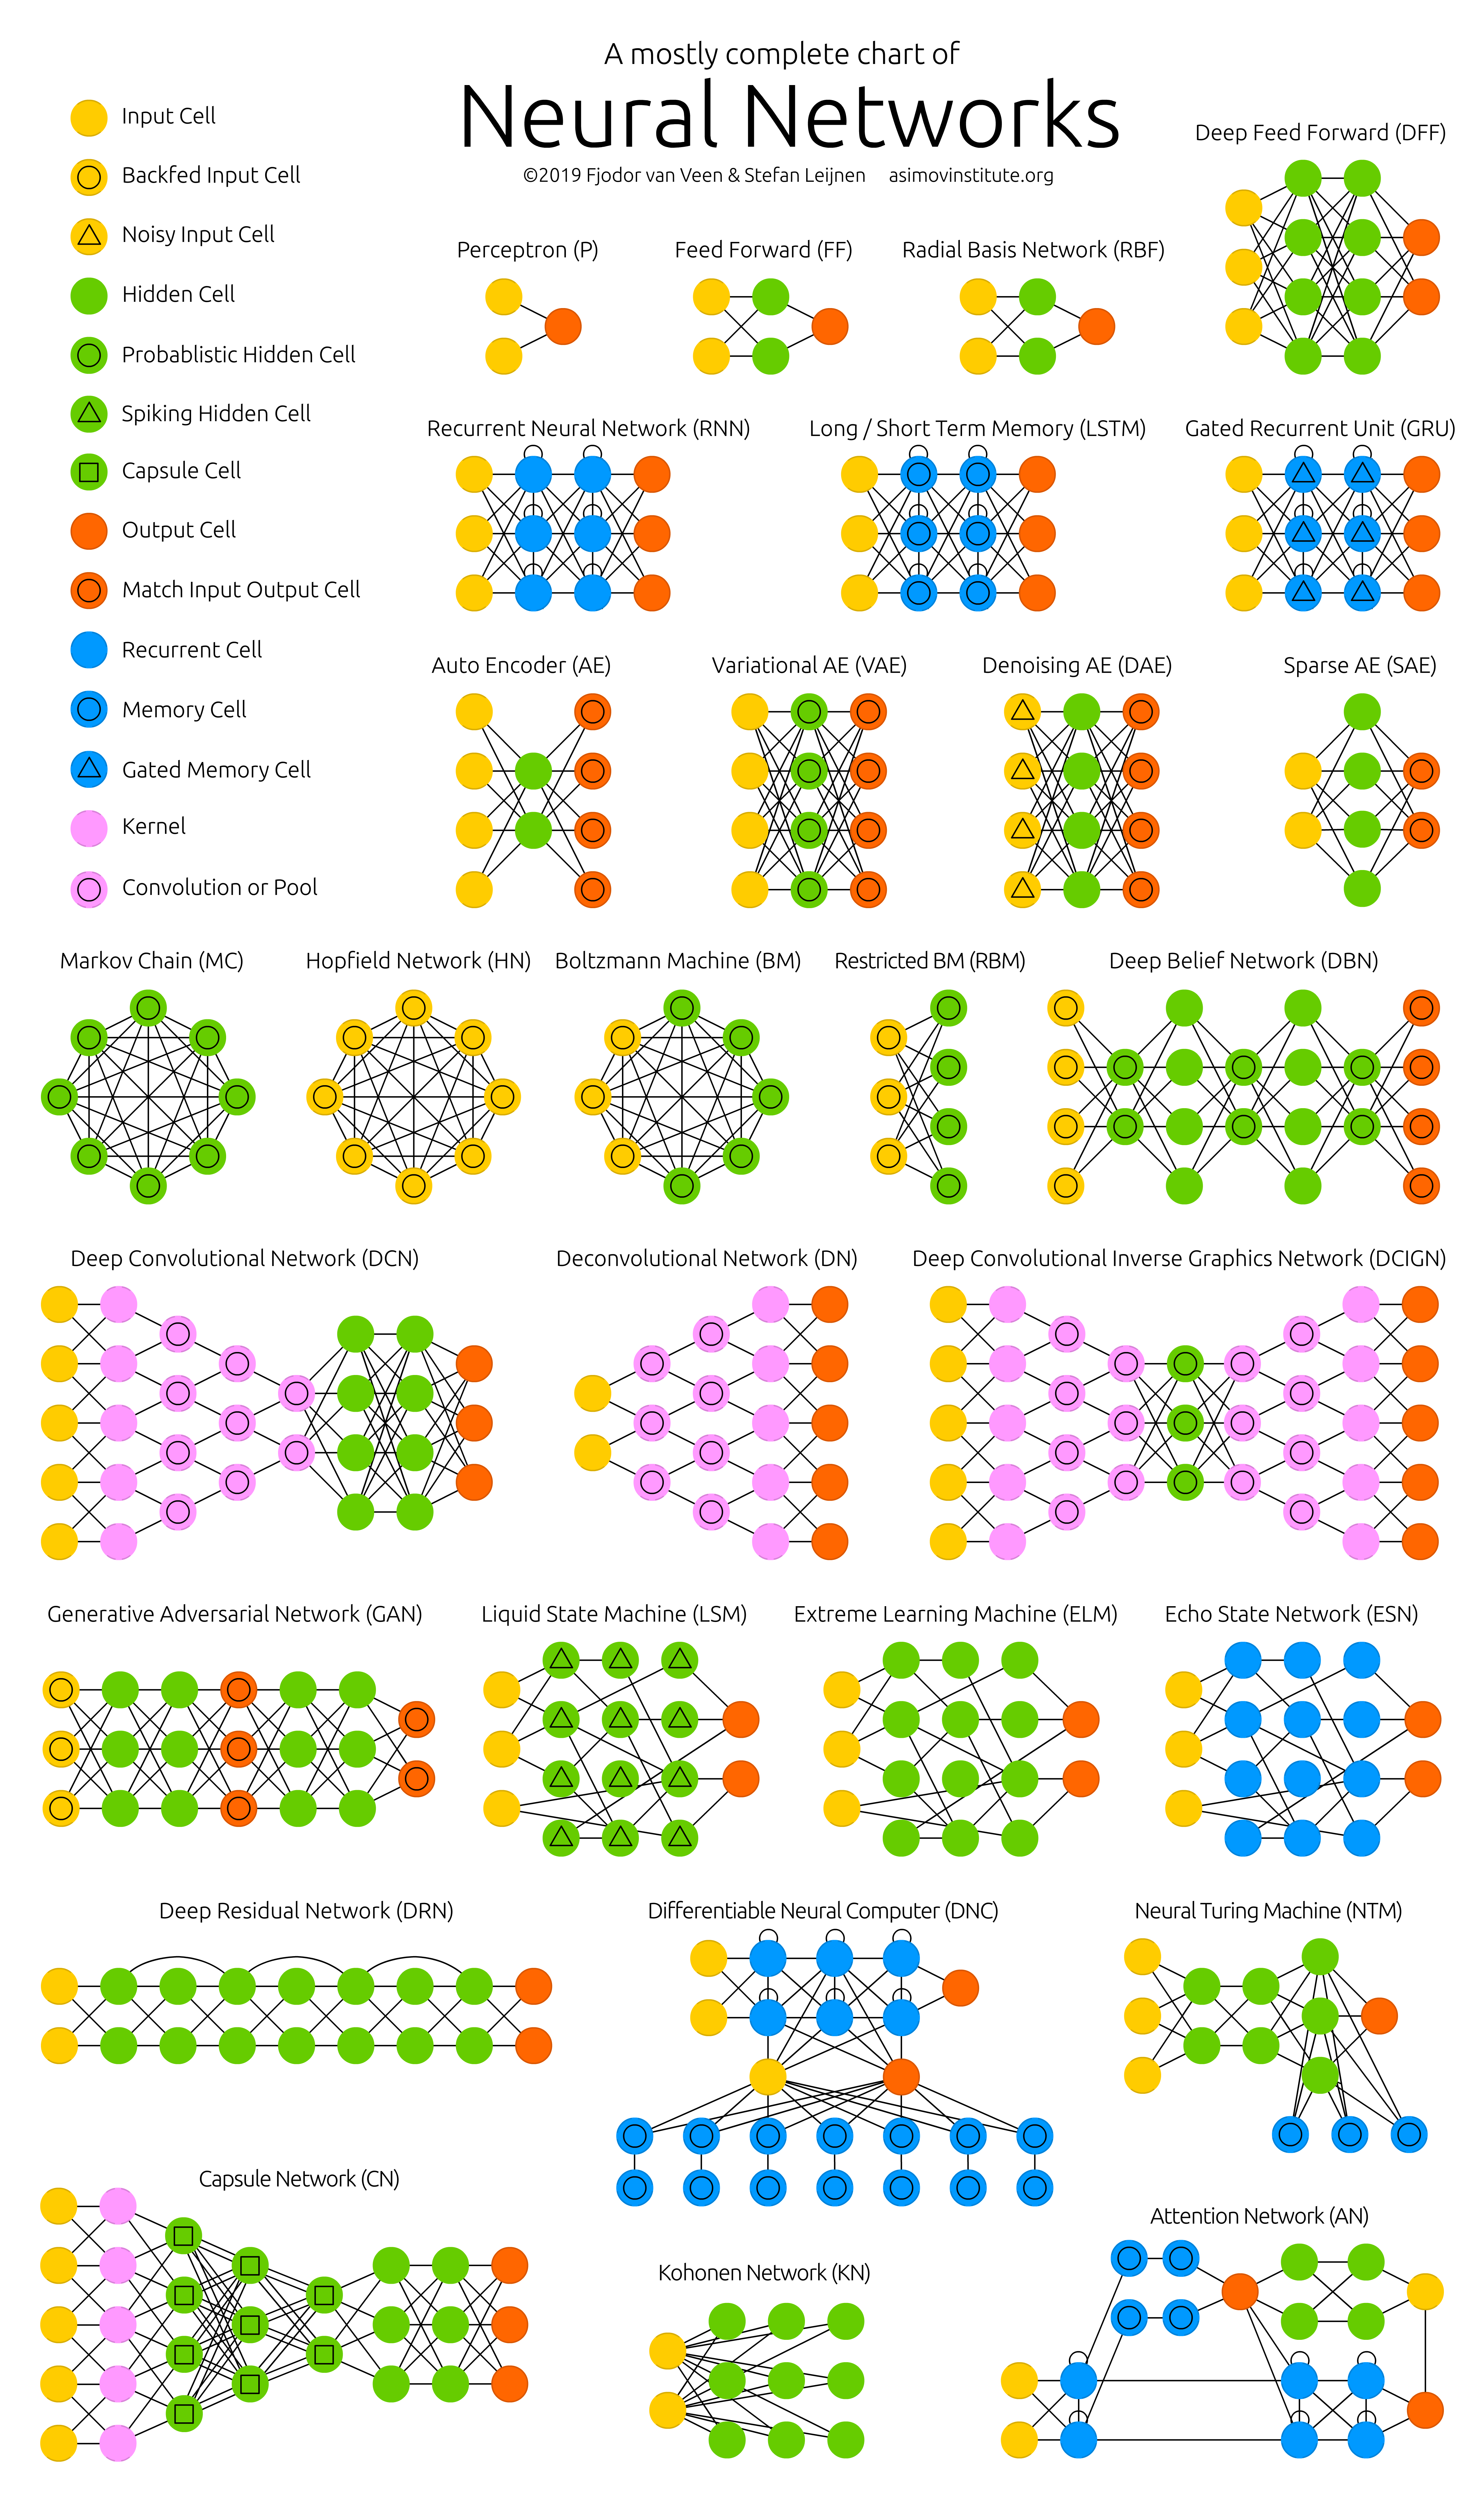
\includegraphics[width=0.8\textwidth]{figures/NeuralNetworkZo19High.png}
    \caption{Topologias de redes neuronales.\\Fuente: \href{https://www.asimovinstitute.org/neural-network-zoo/}{The neural network zoo}}
    \label{fig:NeuralNetworkZo19High}
\end{figure}
% endregion topologias


\subsubsection{El descenso de gradiente \label{gradient-descent}}
% region El descenso de gradiente
% TODO: definición
% TODO: explicar el descenso de gradiente y su problema
% TODO: problema
El problema de desvanecimiento y explosión de gradiente

% endregion El descenso de gradiente


% region GANs
\subsection{Redes generativas adversariales - \textit{Generative Adversarial Networks (GAN)}}
% TODO:
\begin{figure}[H]
    \centering
    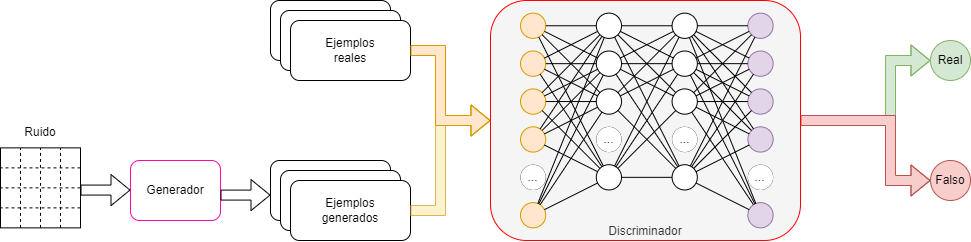
\includegraphics[width=1\textwidth]{figures/chapter02/GANs.drawio.png}
    \caption{Arquitectura de las redes neuronales generativas adversariales.\\Fuente: Elaboración propia.}
    \label{fig:gans-architecture}
\end{figure}
% endregion GANs


% endregion

% region subsection La seguridad de las redes neuronales
\subsection{La seguridad de las redes neuronales}
\label{ch:2:section:state-of-the-art:computer-security-in-neural-networks}

% Dentro de la inteligencia artificial \gls{AI} encontramos el aprendizaje automático \gls{ML} y dentro el aprendijaze profundo \gls{DL}.
% Para el desarrollo de este capítulo limitaremos el alcance del estado del arte de la seguridad informática a los campos relacionados con la inteligencia artificial.

El estado del arte de la seguridad informática es muy complejo por la constante evolución, las ciberamenazas están en constante evolución, los delincuentes informaticos adoptan nuevas técnicas y tácticas para eludir las medidas de seguridad tradicionales, esto tambien le amenaza a las tecnologias que emplean la inteligencia artificial y redes neuronales.

A continuación se explicarán las distintas amenazas que tiene una red neuronal y como puede ser atacada para alterar su comportamiento, posteriormente analizaremos el estado del arte de la inteligencia artificial que se emplea para mejorar la seguridad informática de los dispositivos y de los usuarios.

% Eficiencia
% Invisivilidad
% Efectividad

\subsection{Amenazas de \textit{deep learning}}
\begin{figure}[H]
    \centering
    \centerline{\includesvg[width=1\columnwidth]{figures/chapter02/adversarial-threats.drawio.svg}}
    \caption{Amenazas adversariales.\\Fuente: Elaboración propia.}
    \label{fig:art-adversarial-threats}
\end{figure}

Como podemos observar en la Figura \ref{fig:art-adversarial-threats} existen multitud de amenazas, existen cuatro formas de clasificar las amenazas, está clasificación es en función de como se altera el comportamiento del modelo.

\subsubsection{Evasión}

Busca explotar las vulnerabilidades de la red neuronal para inducir errores en la capacidad de clasificar o de predecir. Se envia información con perturbaciones minimas que alteren notablemente la respuesta del modelo.

\begin{enumerate}
    \item \textbf{Caja blanca}: se conoce todo sobre el modelo, arquitectura, pesos, umbrales, formato de entreada de datos y salida, etc. \cite{learning-machine-learning-part-3-attacking}
    \item \textbf{Caja negra}: se desconoce el modelo, arquitectura, pesos, umbrales, pero se conoce el formato de entrada de datos y la respuesta del modelo. \cite{learning-machine-learning-part-3-attacking}
\end{enumerate}

\subsubsection{Envenenamiento}
% 

Los atacantes intentan manipular los datos de entrenamiento con el objetivo de influir en el resultado del aprendijaze del modelo, esto pueden hacerlo desde distintas etapas.

% $$ \sum_{rand}(x)=\left\{clip\left(x+\delta\right)|\delta\in[-5,5]^{H\times W\times3}\right\} $$

\begin{enumerate}
    \item \textit{Label Flipping Attacks} - Ataques de cambio de etiquetas:
    \item \textit{Clean Label Data Poisoning Attack} - Ataques de envenenamiento de datos de etiquetado limpio:
    \item \textit{Backdoor Attack} - Ataques de puerta trasera: los ataques de puerta trasera, ataques que contienen un disparador, estos se pueden clasificar en tres tipos de escenarios.
          \begin{enumerate}
              \item Aprendizaje d
              \item Aprendizaje por transferencia
              \item Aprendizaje federado
          \end{enumerate}
\end{enumerate}

\paragraph{Label Flipping Attacks}

\paragraph{Clean Label Data Poisoning Attack}


\subparagraph{Feature Collision Attack}
$$x_{p}={\underset{x}{\mathrm{argmin}}}||f\left(x\right)-f\left(x_{t}\right)||_{2}^{2}+\beta||x-x_{b}||_{2}^{2}\,,$$
% 


\subparagraph{Convex Polytope Attack and Bullseye Polytope Attack}

\paragraph{Backdoor Attack}


\subsubsection{Extracción}

Se busca extraer un funcionamiento interno equivalente de la red neuronal, se puede considerar un ataque de ingeniería inversa.

% 
\subsubsection{Inferencia}

\paragraph{Inferencia por Atributos}
\paragraph{Inferencia por Pertenencia}
\paragraph{Inversión de modelos}
\paragraph{Reconstrucción}

\subsection{Defensas contra los ataques en \textit{deep learning}}

\subsubsection{Pre procesamiento}
\subsubsection{Post procesamiento}
\subsubsection{Entrenamiento}
\subsubsection{Transformación}
\paragraph{Evasión}
\paragraph{Envenenamiento}
\subsubsection{Detector}
\paragraph{Evasión}
\paragraph{Envenenamiento}

\subsection{Metricas en los ataques adversariales}

\subsection{\textit{Red team} - \textit{Blue team} en redes neuronales}

Un buen simil entre la seguridad informática clásica y la seguridad en redes neuronales son los conceptos de equipos de ataque y defensa (``red team'' y ``blue team'').

\begin{figure}[H]
    \centering
    \centerline{\includesvg[width=1\columnwidth]{figures/chapter02/ART-for-red-and-blue-teams.drawio.svg}}
    \caption{Ataques y defensas en redes neuronales.\\Fuente: Elaboración propia.}
    \label{fig:art-for-red-and-blue-teams}
\end{figure}

La idea detrás del aprendizaje automático es la de poder predecir modelos predictivos, para ello se usan conjuntos de datos para el entrenamiento.

Los conjuntos de datos se han de procesar, ya que suelen contener mucho ruido, es decir, información muy poco valiosa, errónea o, por el contrario, una alta dimensionalidad de los datos que puede ser contraproducente por no poder reproducir esas medidas o por la poca información que aportan.

Los ataques al aprendizaje automático o profundo suelen estar dirigidos a las distintas etapas de creación y uso de un modelo.

\begin{itemize}
    \item Alteración de los datos de entrada.
    \item Alteración del proceso de aprendizaje.
    \item Extración de los datos de entrenamiento.
    \item Bloqueo del modelo.
\end{itemize}

Durante el transcurso del trabajo discutiremos los siguientes ataques y defensas previamente en la sección \nameref{ch:2:section:state-of-the-art:computer-security-in-neural-networks} que se pueden usar en los modelos.

\begin{itemize}
    \item Envenenamiento de datos.
    \item Puerta trasera.
    \item Extracción de datos
    \item Ingeniería inversa.
    \item Evasión.
\end{itemize}

Se puede ser categorizar la seguridad de los modelos con el modelado \gls{STRIDE} de microsoft\footnote{Modelado de amenazas de microsoft \href{https://learn.microsoft.com/es-es/azure/security/develop/threat-modeling-tool-threats}{Enlace}} o con la matriz \gls{MITRE}.

\begin{table}[H]
    \centering
    \small
    \begin{tabularx}{\textwidth}{|l|X|}
        \hline
        \textbf{Amenaza}    & \textbf{Tipo de ataque}                                           \\
        \hline
        Corrupción de datos & Ataques de envenenamiento de datos, ataques de puerta trasera     \\
        Extracción de datos & Ataques de inferencia de membresía, ataques de ingeniería inversa \\
        Denegación          & Ataques de envenenamiento de datos                                \\
        \hline
    \end{tabularx}
    \caption{Amenazas STRIDE relacionadas con la seguridad de la IA}
    \label{tab:amenazas}
\end{table}

% endregion

% region subsection Las redes neuronales para la seguridad informática
\subsection{Las redes neuronales para la seguridad informática}
% TODO: aplicaciones reales de ciberseguridad que usan inteligencia artificial 


% endregion




\subsection{Normativa y estándares}
% https://eur-lex.europa.eu/resource.html?uri=cellar:e0649735-a372-11eb-9585-01aa75ed71a1.0008.02/DOC_1&format=PDF
% https://eur-lex.europa.eu/resource.html?uri=cellar:e0649735-a372-11eb-9585-01aa75ed71a1.0008.02/DOC_2&format=PDF

% Según la unión europea toda la seguridad es este apartado :ok: 
% (51) La ciberseguridad es fundamental para garantizar que los sistemas de IA resistan a las actuaciones de terceros maliciosos que, aprovechando las vulnerabilidades del sistema, traten de alterar su uso, conducta o funcionamiento o de poner en peligro sus propiedades de seguridad. Los ciberataques contra sistemas de IA pueden dirigirse contra elementos específicos de la IA, como los conjuntos de datos de entrenamiento (p. ej., contaminación de datos) o los modelos entrenados (p. ej., ataques adversarios), o aprovechar las vulnerabilidades de los elementos digitales del sistema de IA o la infraestructura de TIC subyacente. Por lo tanto, para asegurar un nivel de ciberseguridad adecuado a los riesgos, los proveedores de sistemas de IA de alto riesgo deben adoptar medidas adecuadas teniendo también en cuenta, cuando proceda, la infraestructura de TIC subyacente.









% https://www.youtube.com/@felipebravom



% Feb 1990: Generative Adversarial Networks / Curiosity Generative Adversarial Networks (GANs) have become very popular.[MOST] They were first published in 1990 in Munich under the moniker Artificial Curiosity. [AC90-20][GAN1] Two dueling NNs (a probabilistic generator and a predictor) are trying to maximize each other's loss in a minimax game.[AC](Sec. 1) The generator (called the controller) generates probabilistic outputs (using stochastic units[AC90] like in the much later StyleGANs[GAN2]). The predictor (called the world model) sees the outputs of the controller and predicts environmental reactions to them. Using gradient descent, the predictor NN minimizes its error, while the generator NN tries to make outputs that maximize this error: one net's loss is the other net's gain.[AC90] (The world model can also be used for continual online action planning.[AC90][PLAN2-3][PLAN])

% 4 years before a 2014 paper on GANs,[GAN1] my well-known 2010 survey[AC10] summarised the generative adversarial NNs of 1990 as follows: a "neural network as a predictive world modelis used to maximize the controller's intrinsic reward, which is proportional to the model's prediction errors" (which are minimized).

% The 2014 GANs are an instance of this where the trials are very short (like in bandit problems) and the environment simply returns 1 or 0 depending on whether the controller's (or generator's) output is in a given set.[AC20][AC][T22](Sec. XVII)

% Other early adversarial machine learning settings[S59][H90] were very different—they neither involved unsupervised NNs nor were about modeling data nor used gradient descent.

% The 1990 principle has been widely used for exploration in Reinforcement Learning[SIN5][OUD13] [PAT17][BUR18] and for synthesis of realistic images,[GAN1,2] although the latter domain was recently taken over by Rombach et al.'s Latent Diffusion, another method published in Munich,[DIF1] building on Jarzynski's earlier work in physics from the previous millennium[DIF2]  and more recent papers.[DIF3-5]

% In 1991, I published yet another ML method based on two adversarial NNs called Predictability Minimization for creating disentangled representations of partially redundant data, applied to images in 1996.

\clearpage\thispagestyle{empty}\cleardoublepage

% \chapter{OBJETIVOS}


\section{Analisis}

\section{Ataques}

\section{Defensas}
% \clearpage\thispagestyle{empty}\cleardoublepage

% \chapter{MATERIALES Y MÉTODOS}

\begin{lstlisting}[language=docker-compose-2,caption={Example docker-compose.yml},breaklines=true,label={code:compose}]
version: '2'
services:
  web:
     build: .
     ports:
        - "5000:5000"
     volumes:
        - .:/code
        - logvolume01:/var/log
     links:
        - redis
  redis:
     image: redis
volumes:
    logvolume01: {}
\end{lstlisting}


\section{Análisis}

\section{Ataques}

\section{Defensas}


% \clearpage\thispagestyle{empty}\cleardoublepage

% \chapter{RESULTADOS}

% \clearpage\thispagestyle{empty}\cleardoublepage

% \chapter{CONCLUSIONES}

% \cite{devops-redhat}

% \emoji{woman-health-worker-medium-skin-tone}


% Ââ Êê Îî Ôô Ŵŵ Ŷŷ Ïï

% Ăă Ĕĕ Ĭĭ Ŏŏ Ŭŭ

% Āā Ēē Īī Ōō Ūū Ȳȳ

% \gls{latex}
% \clearpage\thispagestyle{empty}\cleardoublepage

\clearpage

\printglossaries
% ===== Configuración de la bibliografía

\pagenumbering{roman}  % Numeración romana para el índice
\bibliographystyle{unsrtnat}
\bibliography{bibliography.bib}
\addcontentsline{toc}{chapter}{Bibliografía}
\nocite{*}

\end{document}